% !TEX root = ../thesis.tex

\section{Comparison of Simulation to Data}
\label{sec:comp}

% Comparison between MC and data
A crucial check on the validity of our selection cuts and categorizations is to compare the MC samples to the data in the regions where no signal is expected to be observed.
In this section, we review the data to MC comparisons for relevant kinematic distributions by looking at control plots in non-signal regions.
We define two control regions of the analysis as follows: a jet mass sideband and a top-enriched control region.

% Jet mass sideband
The jet mass sideband applies the final event selection cuts of subsection~\ref{subsec:eventSelect}, but with the \MJ selection cuts $20<\MJ<70\unit{GeV}$ or $150<\MJ<210\unit{GeV}$, so that the \Vhad large-radius jets present do not originate from a corresponding \VorH decay in signal events.
To correct modeling of fake $V$ jets at low \pt, we also define a separate \Wjets dominated sideband of $30<\MJ<50\unit{GeV}$ that is used to derive rescaling factors for the \Wjets background yields.
These rescaling factors are applied to \Wjets background yields for the analysis.

% Top-enriched control region
The top-enriched control region is used to calibrate the performance of the soft drop algorithm and jet substructure variables on merged bosons.
We define this region to be enriched in $t\bar{t}$ and single top events, where the selected large-radius jet results from an actual hadronically decaying $W$ boson.
This is done by applying the selection cuts of subsection~\ref{subsec:eventSelect}, but with an inverted $b$-tag veto to ensure the presence of at least one standard AK4 $b$-tagged jet in the event.
The resulting event sample is therefore largely dominated by $t\bar{t}$ and single top events.
%From this we obtain $b$-tagging scale factors and top \pt reweighting values that are applied in the rest of the analysis.

\subsection{Control Plots}

% Run 2 control plots
The control plots presented here run over the full dataset from 2017, 2017, and 2018.
These plots were produced using separate MC samples for each year that are combined and weighted by their individual luminosities.

\subsubsection{Control Plots in the Jet Mass Sideband Region}

% Jet mass sideband control plots
Figure~\ref{fig:SB_controlPlotsRun2_1} shows kinematic variables related to the lepton candidate, such as the \pt, $\eta$, and \ptmiss, for both $e$ and $\mu$ channels.
In figure~\ref{fig:SB_controlPlotsRun2_2}, the distributions correspond to the \pt and transverse mass of the \Wlep candidate, along with the diboson invariant mass \MVV, again for both $e$ and $\mu$ channels.
For figure~\ref{fig:SB_controlPlotsRun2_3}, the distributions show the \pt, $\eta$, \MJ, \nsubjDDT, and \DoubleB of the large-radius jet from the \Vhad candidate.
Finally, for figure~\ref{fig:SB_controlPlotsRun2_4}, the \VBF-related distributions are shown for \DetaVBF, \mjjVBF, \nJets, and \Dy.
The rescaling factors applied to the \Wjets background yields are 0.96, 0.86, and 0.79 for 2016, 2017, and 2018, respectively.

\begin{figure}[htbp]
  \centering
  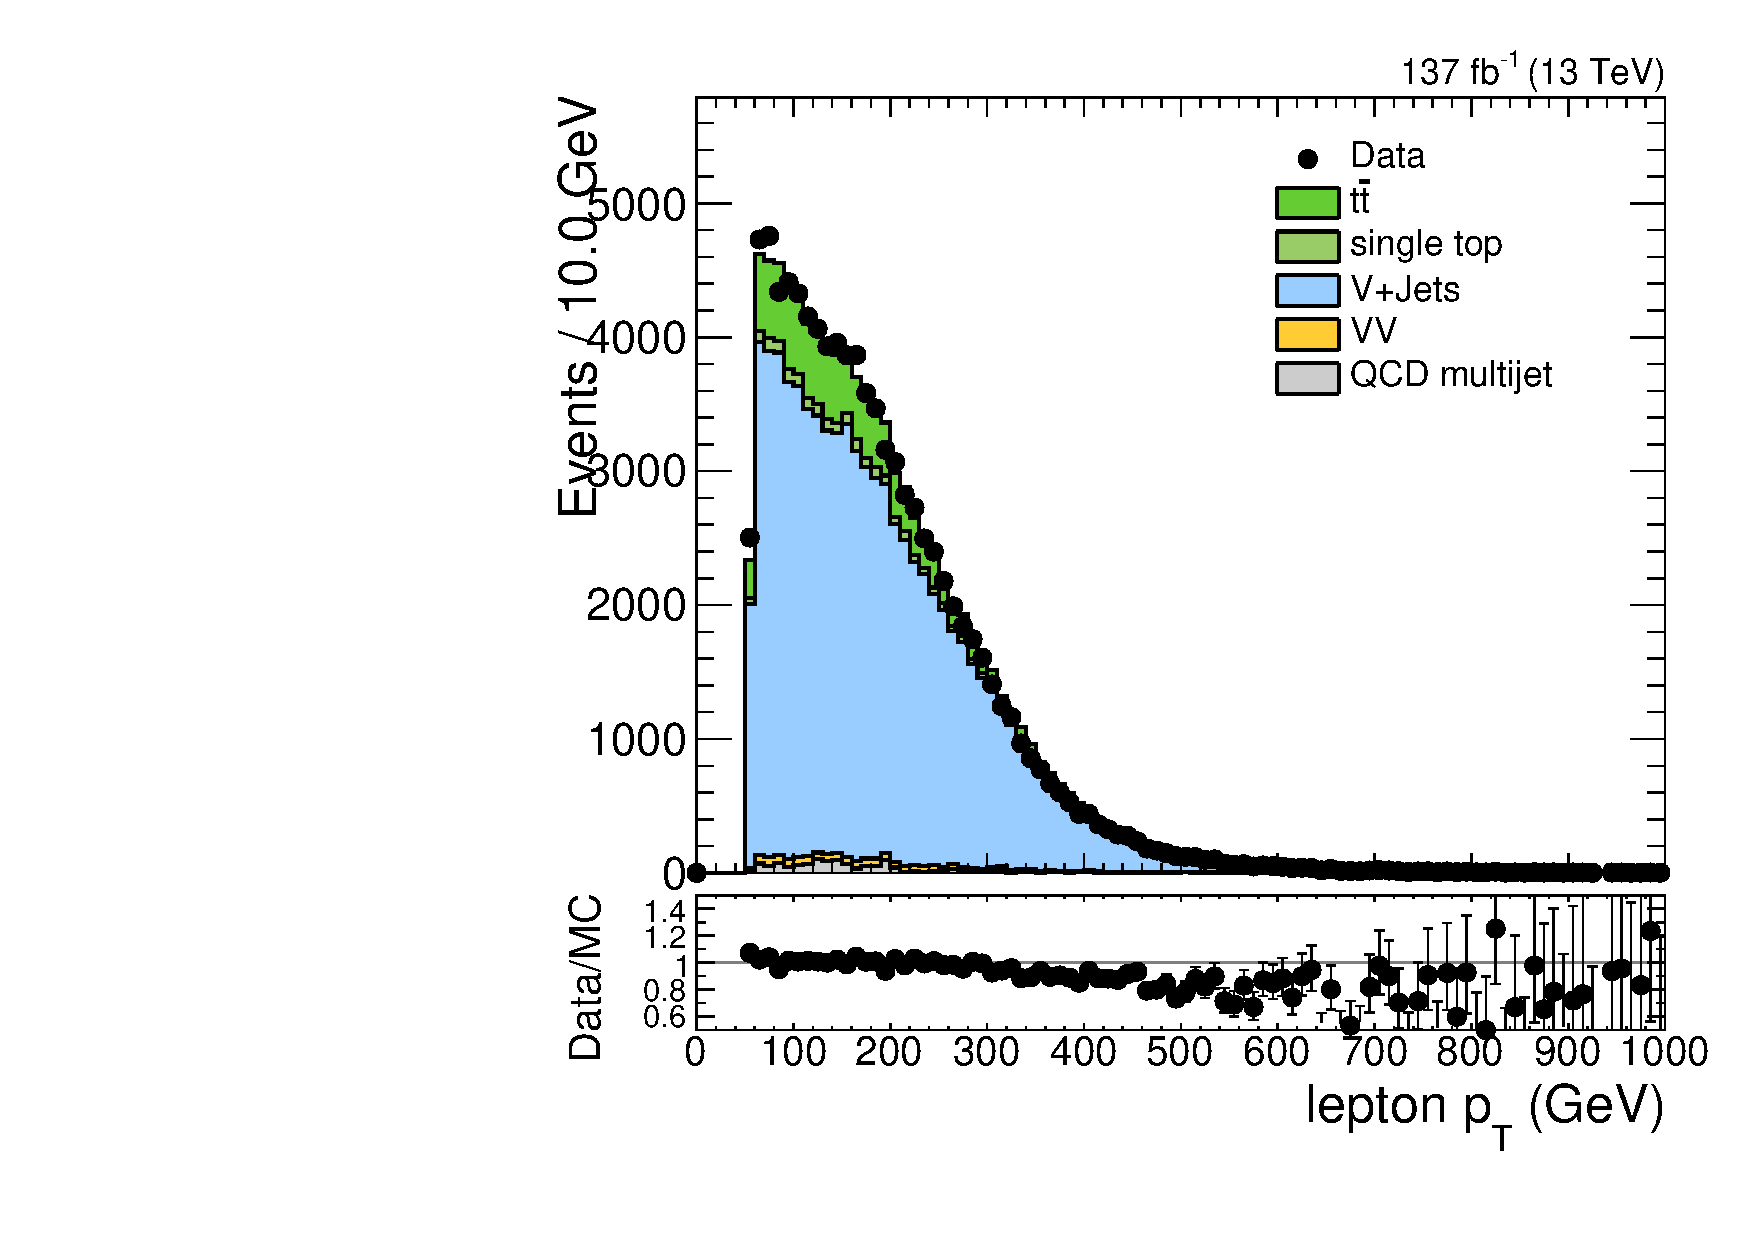
\includegraphics[width=0.3825\textwidth]{fig/controlPlots/SB_b1_mu_allP_allC_allD_Run2_lnujj_l1_l_pt.pdf}
  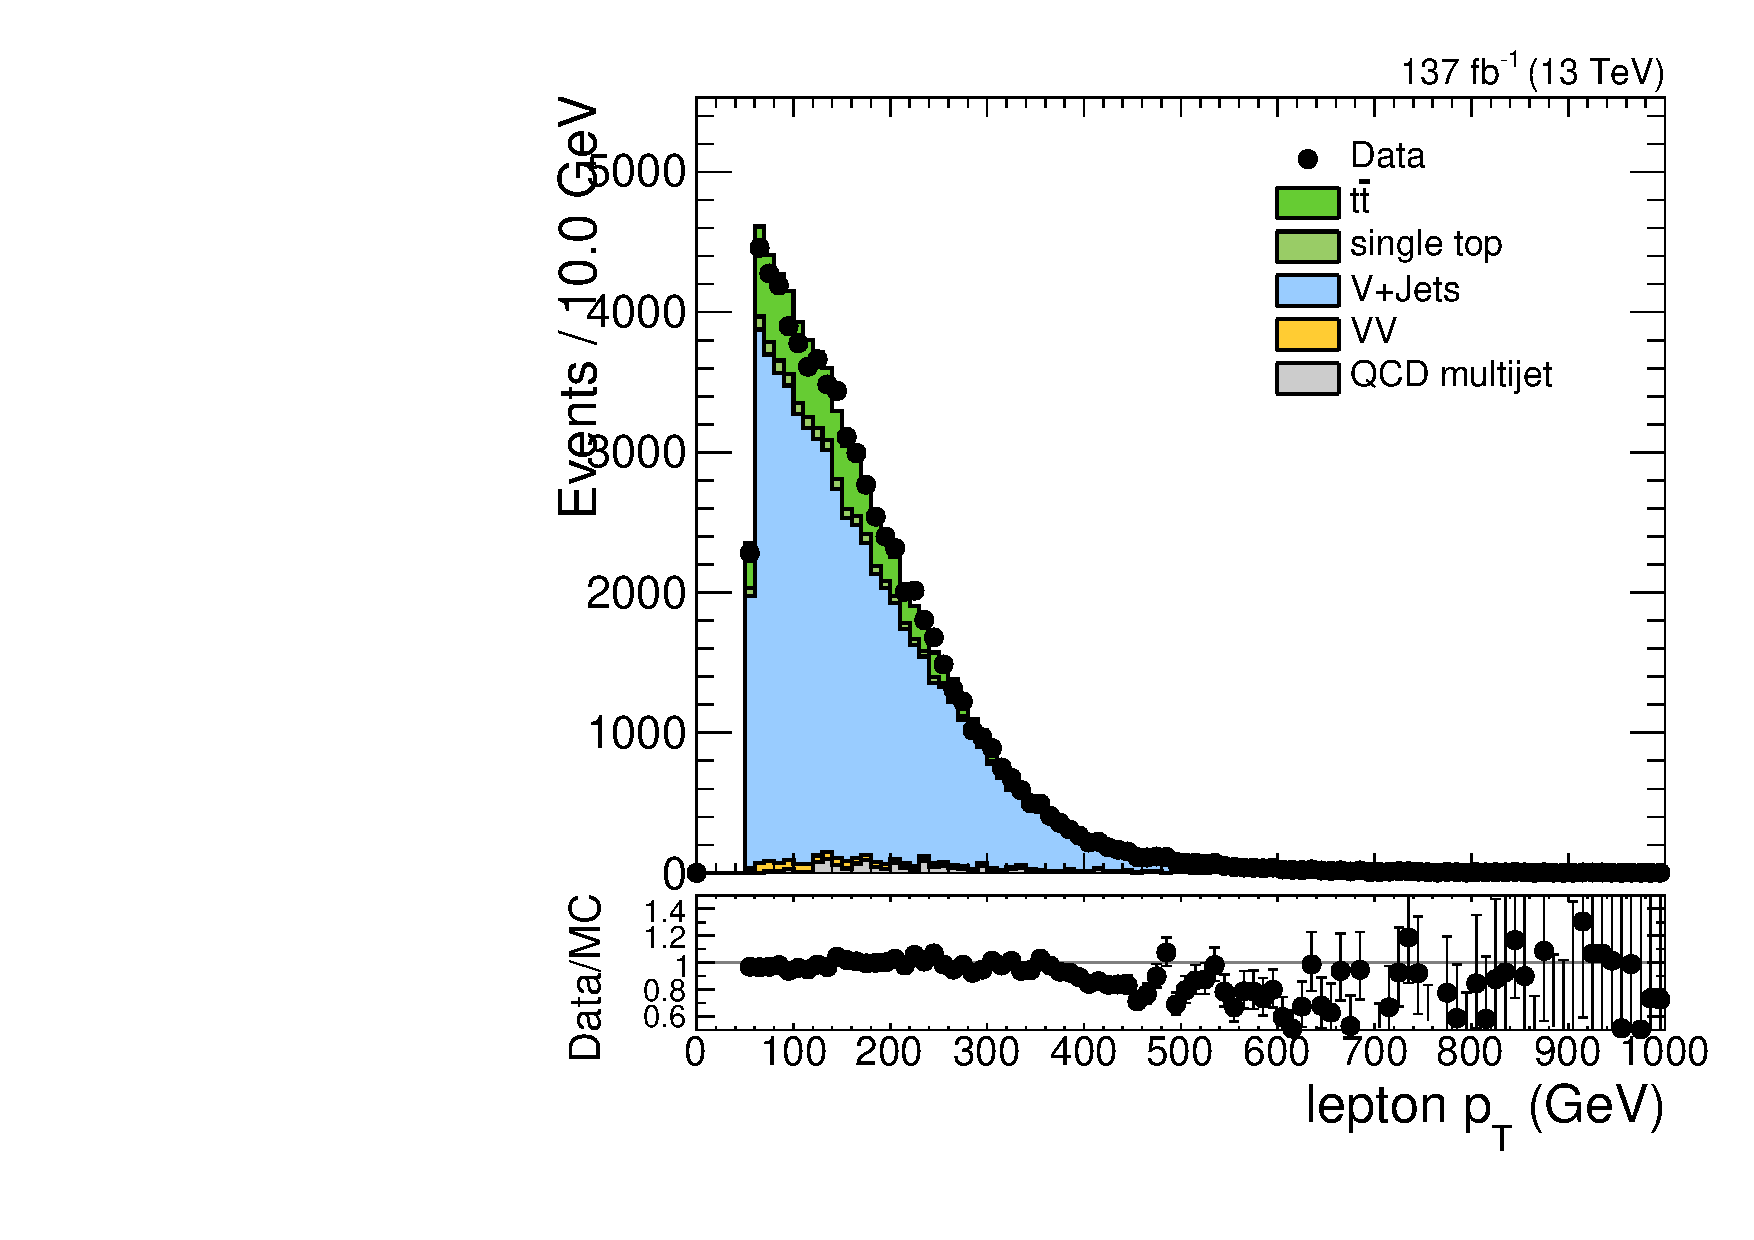
\includegraphics[width=0.3825\textwidth]{fig/controlPlots/SB_b1_e_allP_allC_allD_Run2_lnujj_l1_l_pt.pdf}\\
  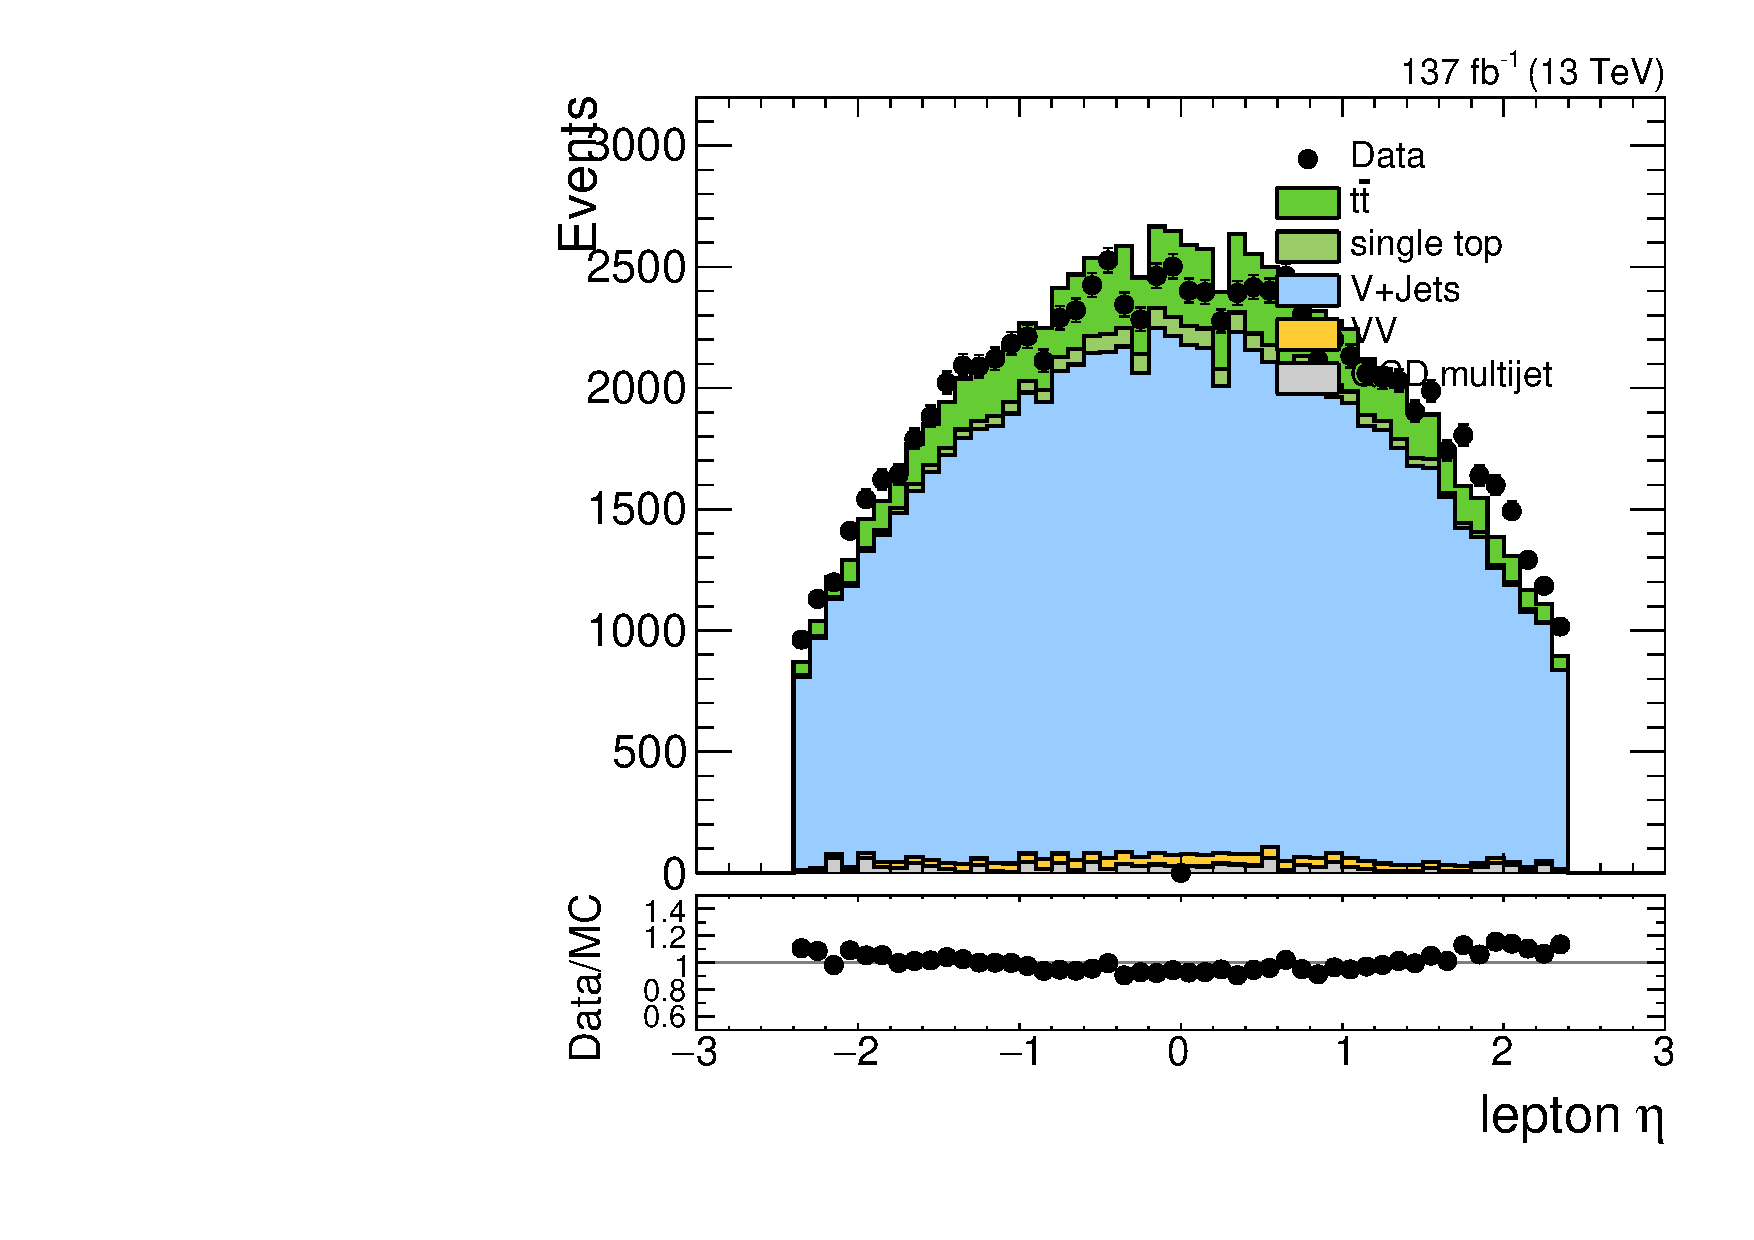
\includegraphics[width=0.3825\textwidth]{fig/controlPlots/SB_b1_mu_allP_allC_allD_Run2_lnujj_l1_l_eta.pdf}
  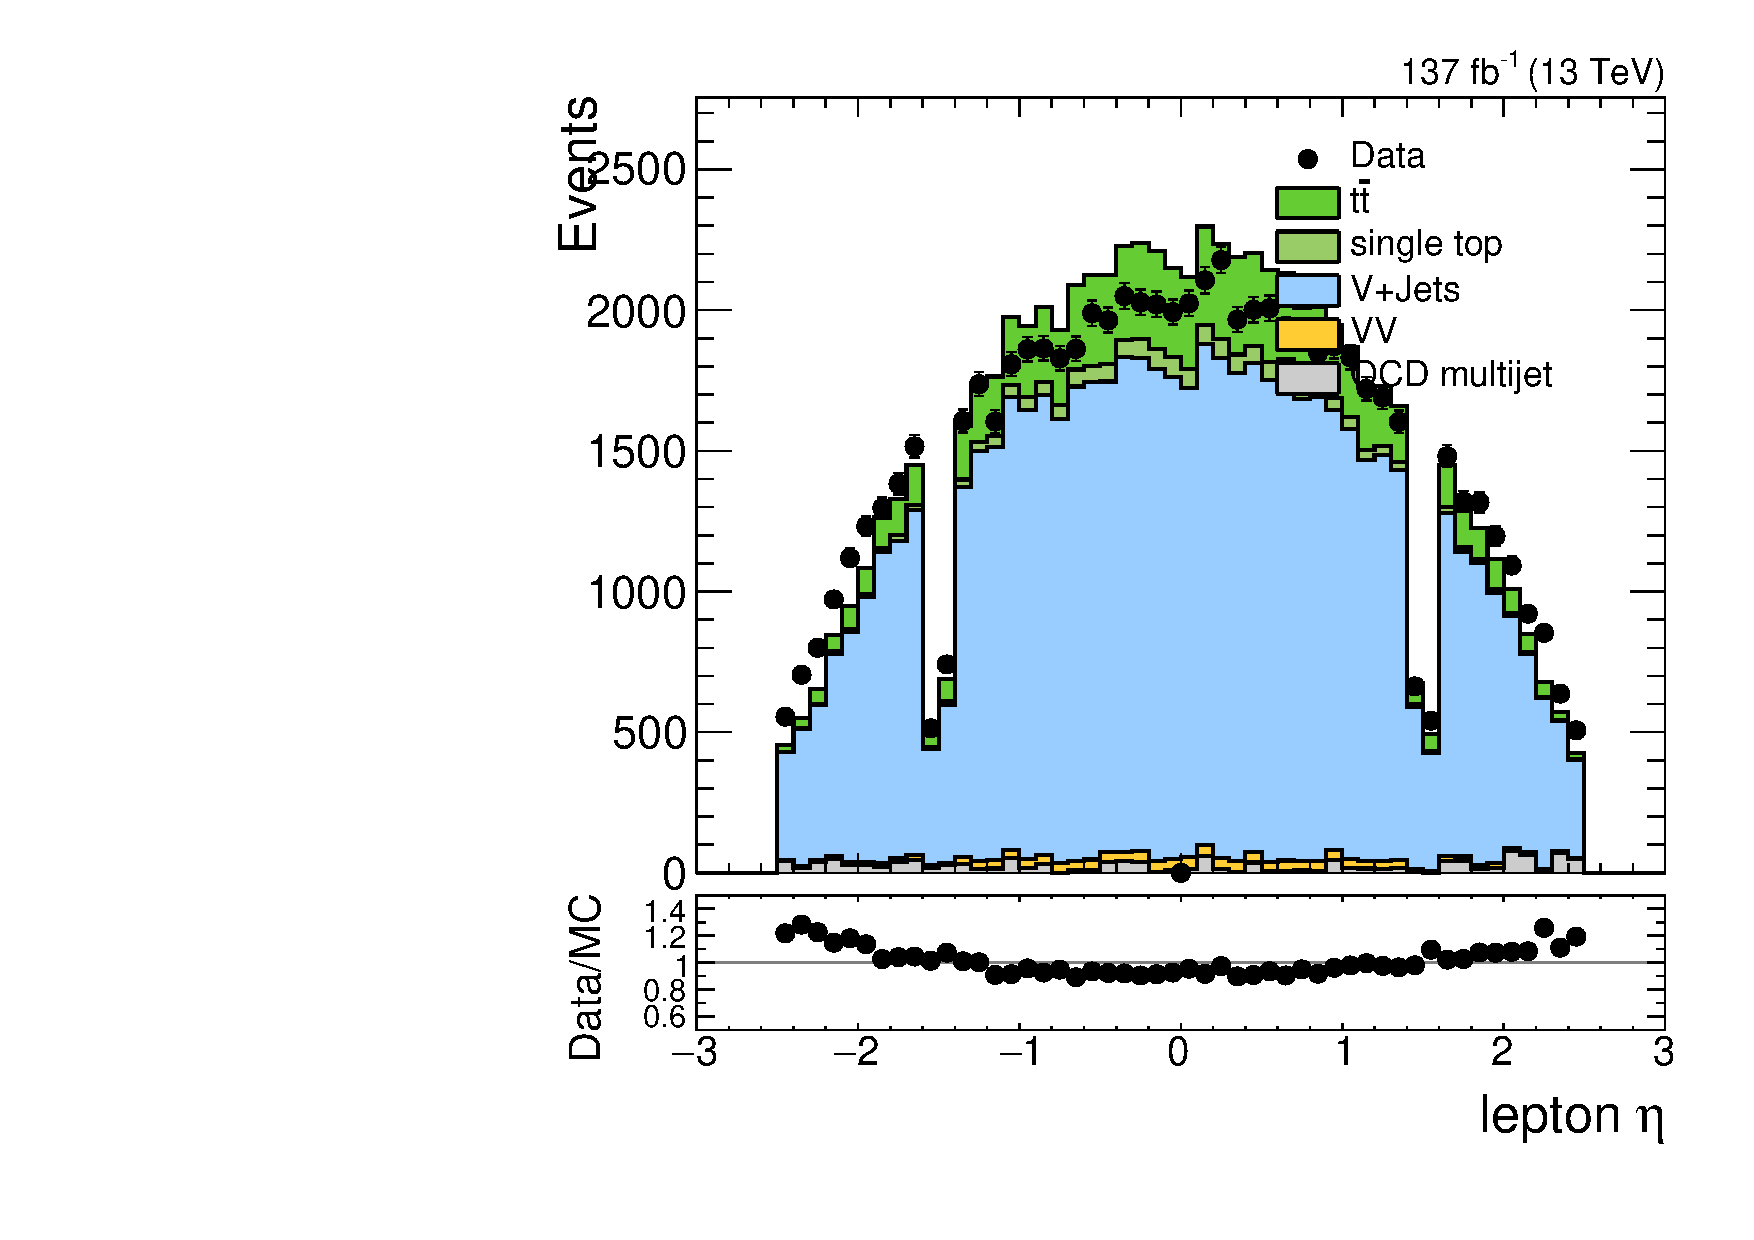
\includegraphics[width=0.3825\textwidth]{fig/controlPlots/SB_b1_e_allP_allC_allD_Run2_lnujj_l1_l_eta.pdf}\\
  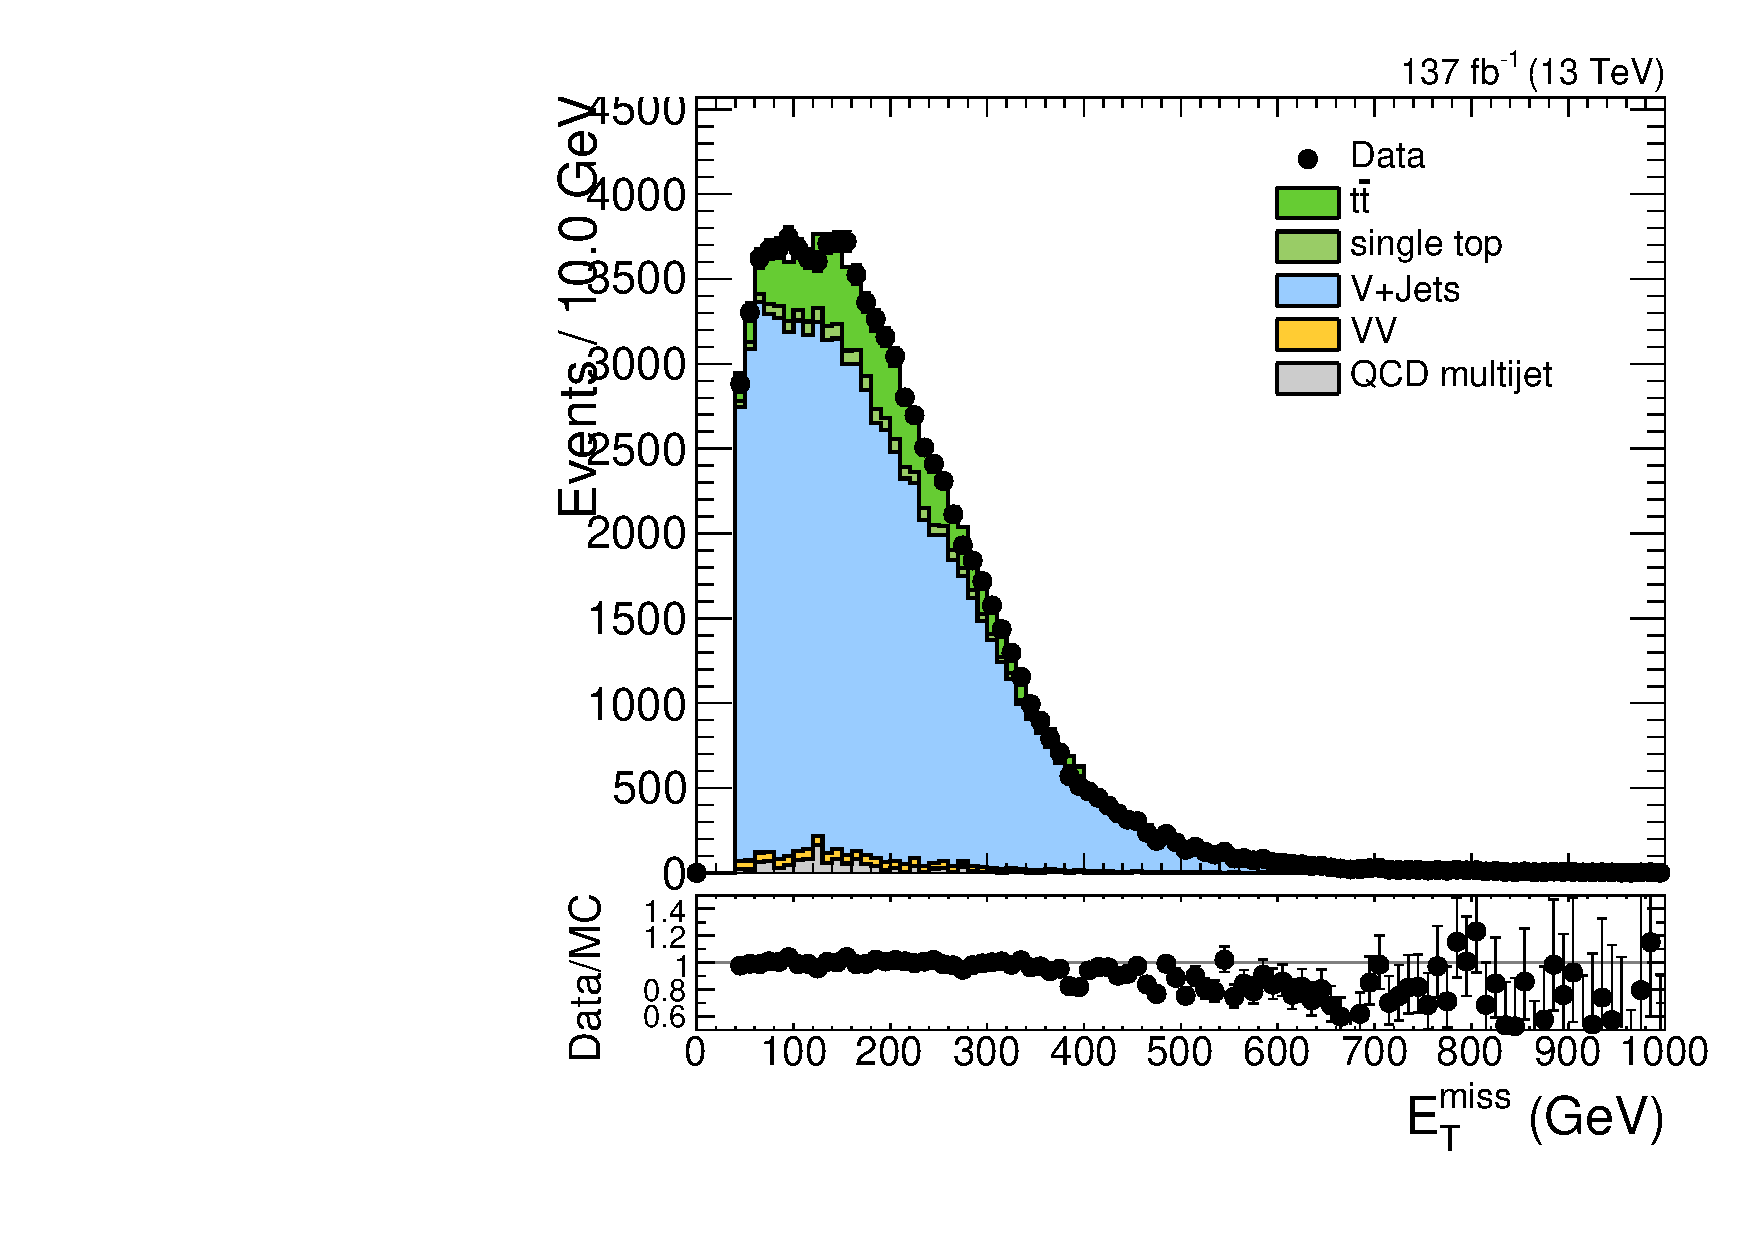
\includegraphics[width=0.3825\textwidth]{fig/controlPlots/SB_b1_mu_allP_allC_allD_Run2_met_pt.pdf}
  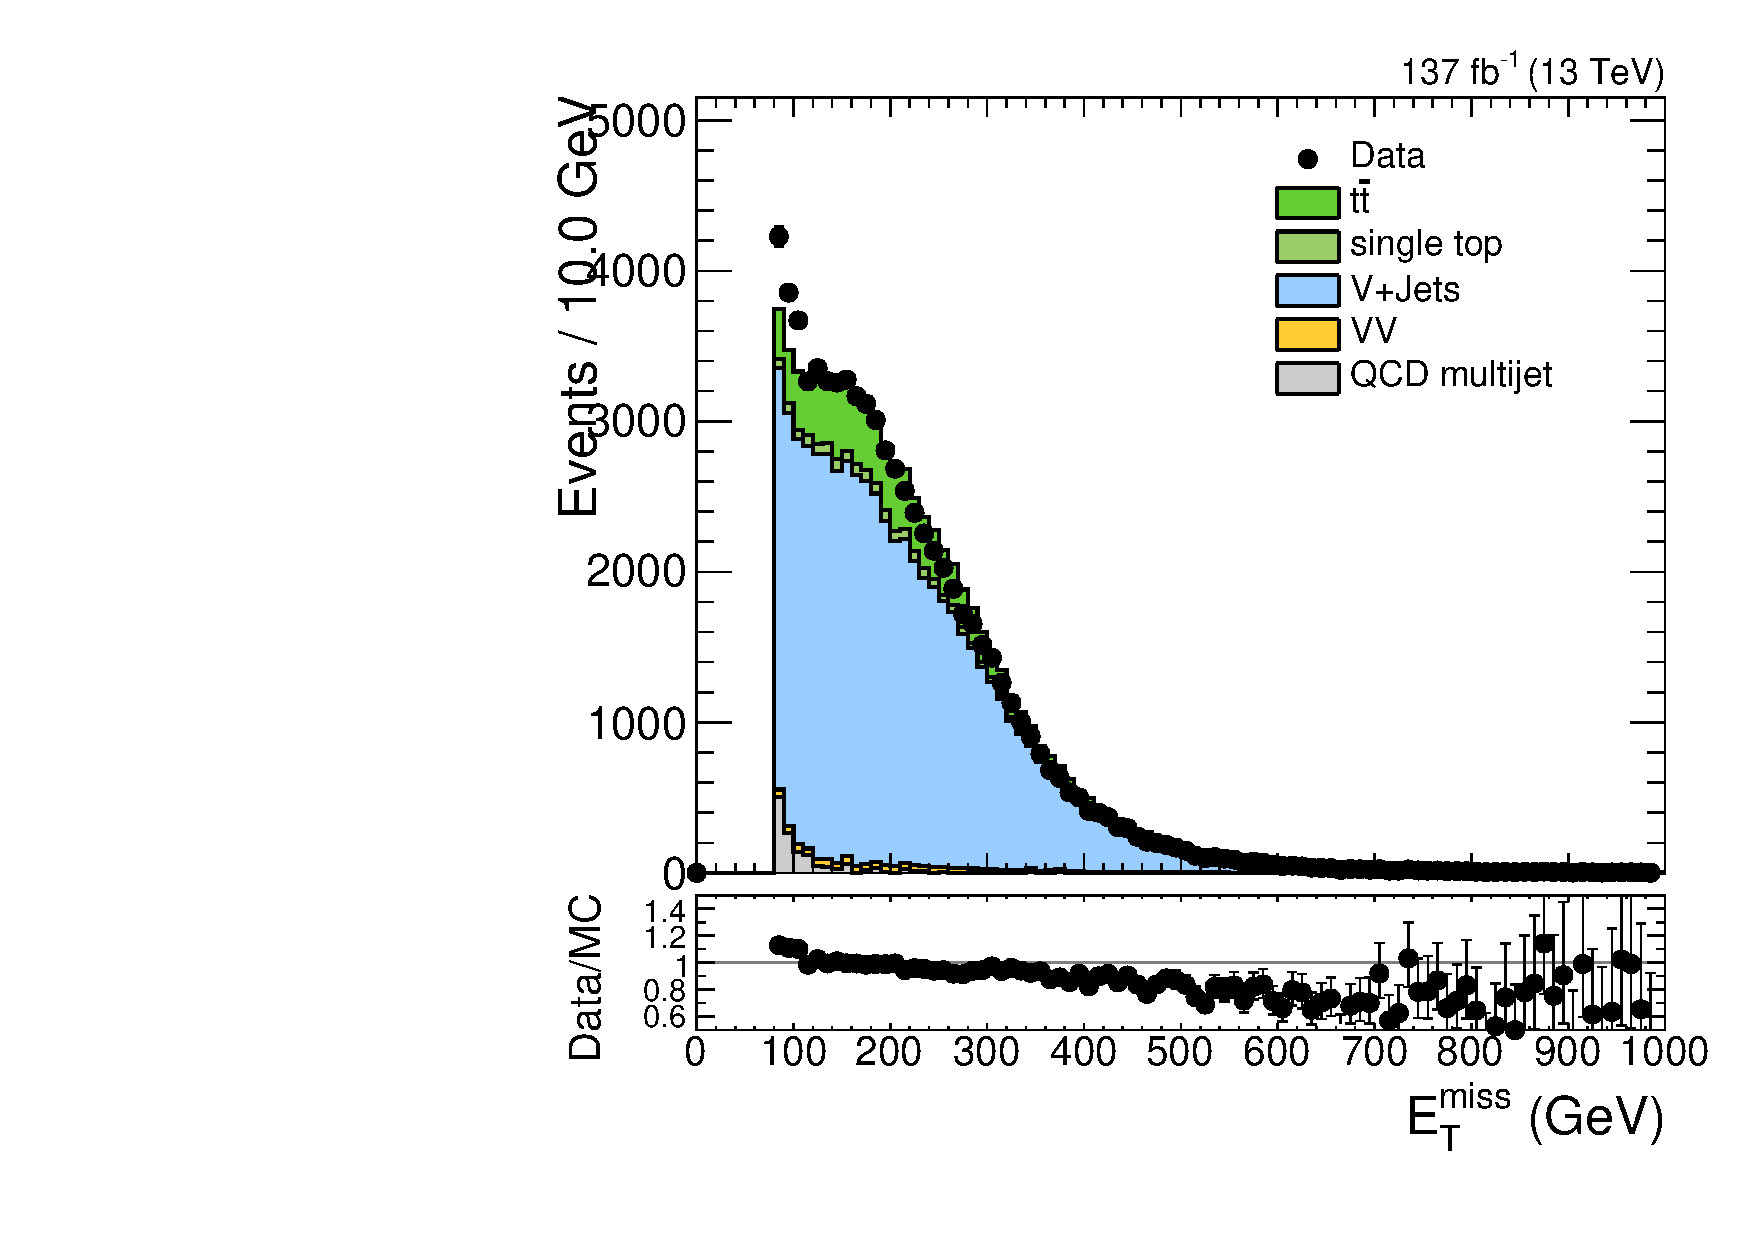
\includegraphics[width=0.3825\textwidth]{fig/controlPlots/SB_b1_e_allP_allC_allD_Run2_met_pt.pdf}\\
  \caption{
    Comparison plots between data and MC from Run 2 for different \Wlep-related observables, in the jet mass sideband.
    From top to bottom: lepton \pt, lepton $\eta$, \ptmiss.
    Left: muon channel, right: electron channel.
  }
  \label{fig:SB_controlPlotsRun2_1}
\end{figure}

\begin{figure}[htbp]
  \centering
  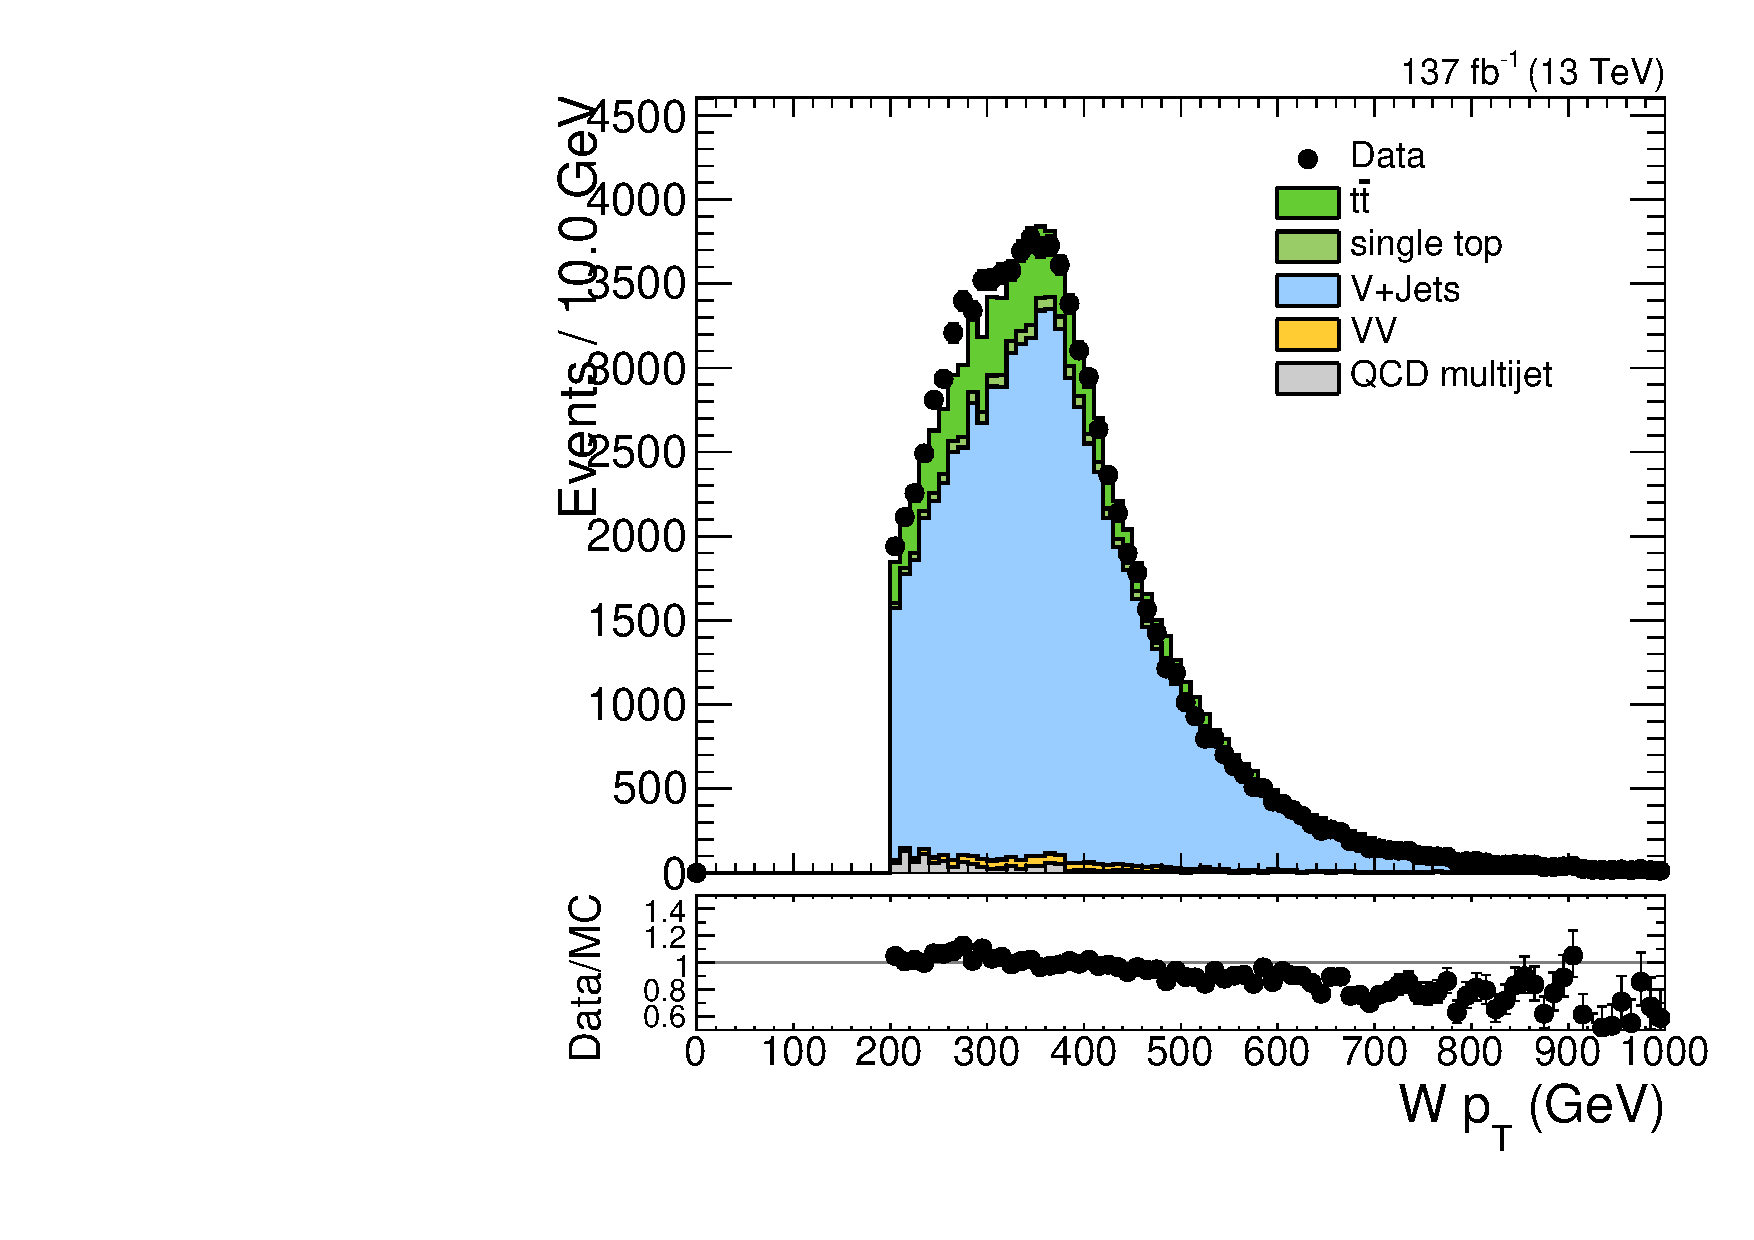
\includegraphics[width=0.3825\textwidth]{fig/controlPlots/SB_b1_mu_allP_allC_allD_Run2_lnujj_l1_pt.pdf}
  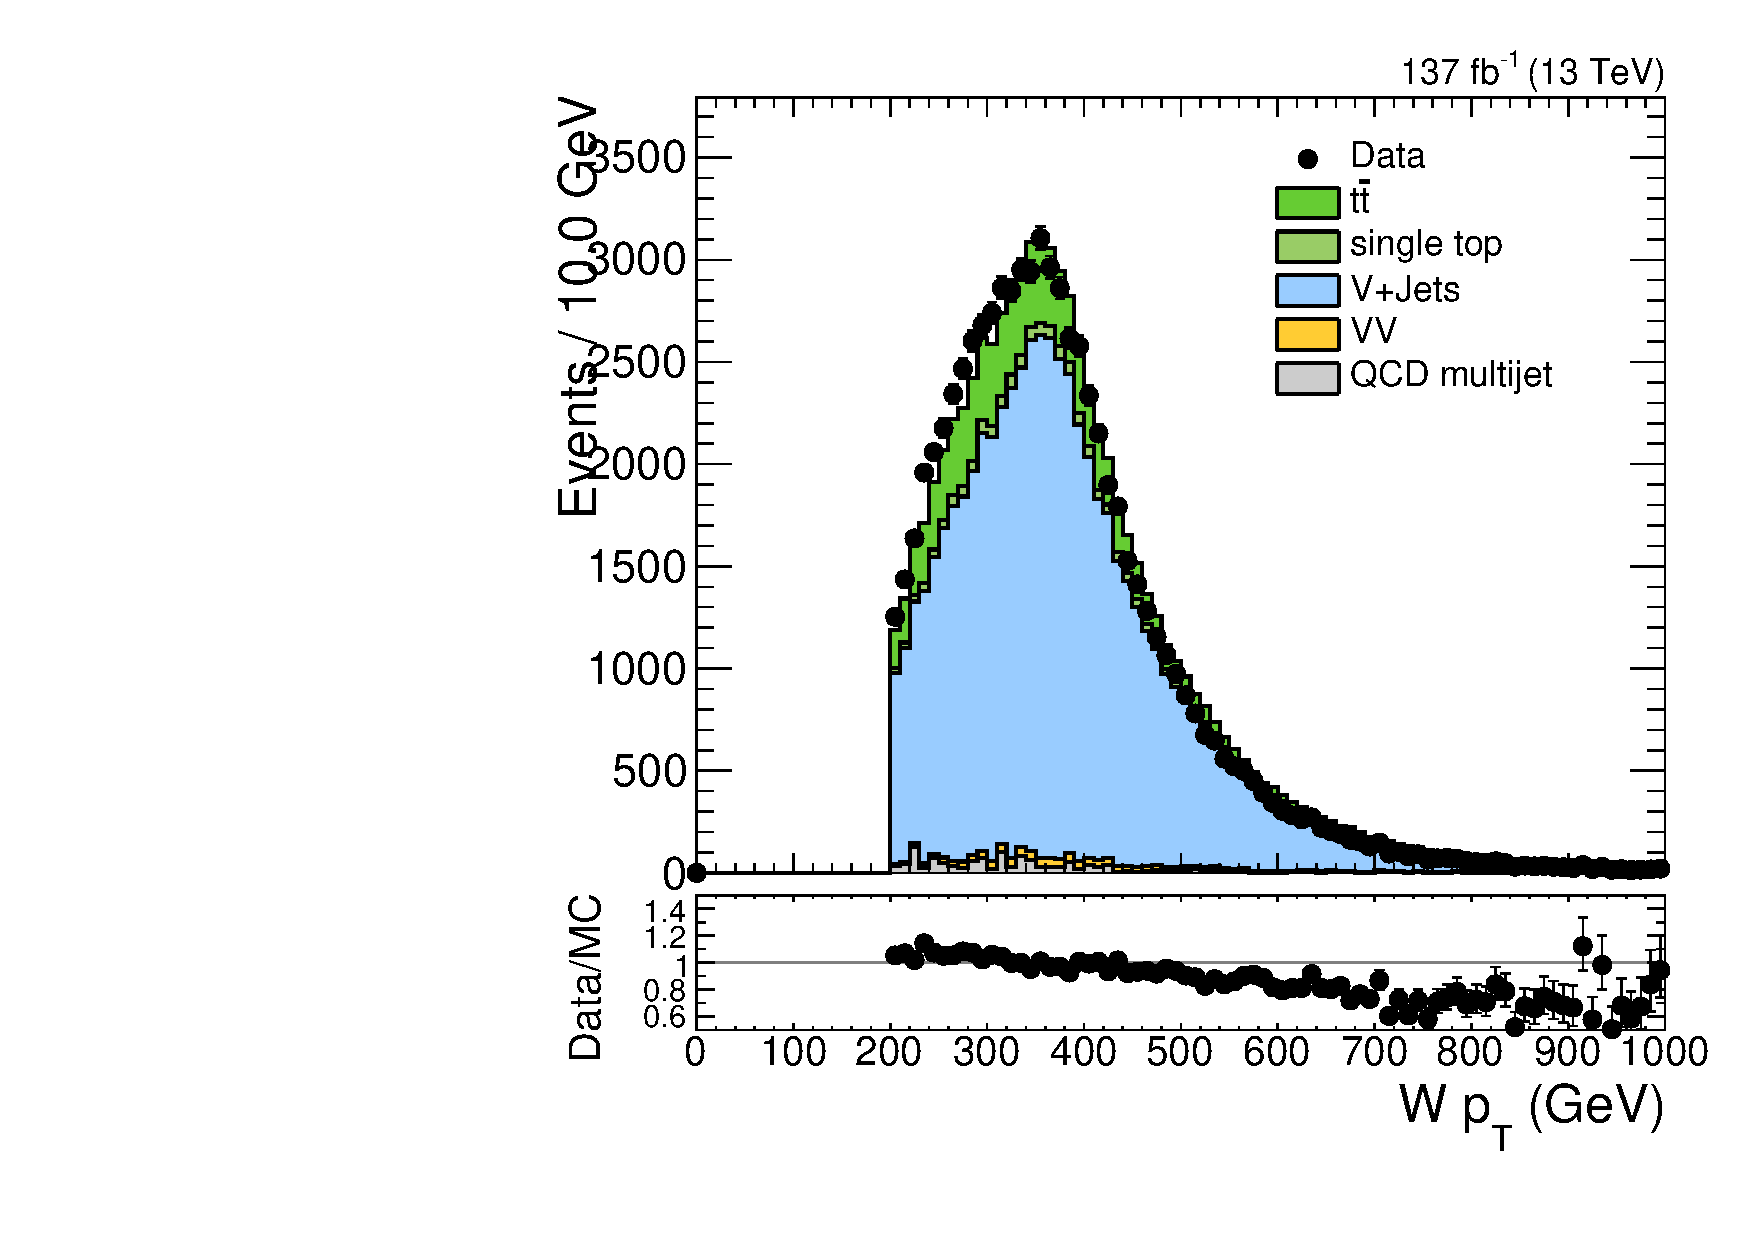
\includegraphics[width=0.3825\textwidth]{fig/controlPlots/SB_b1_e_allP_allC_allD_Run2_lnujj_l1_pt.pdf}\\
  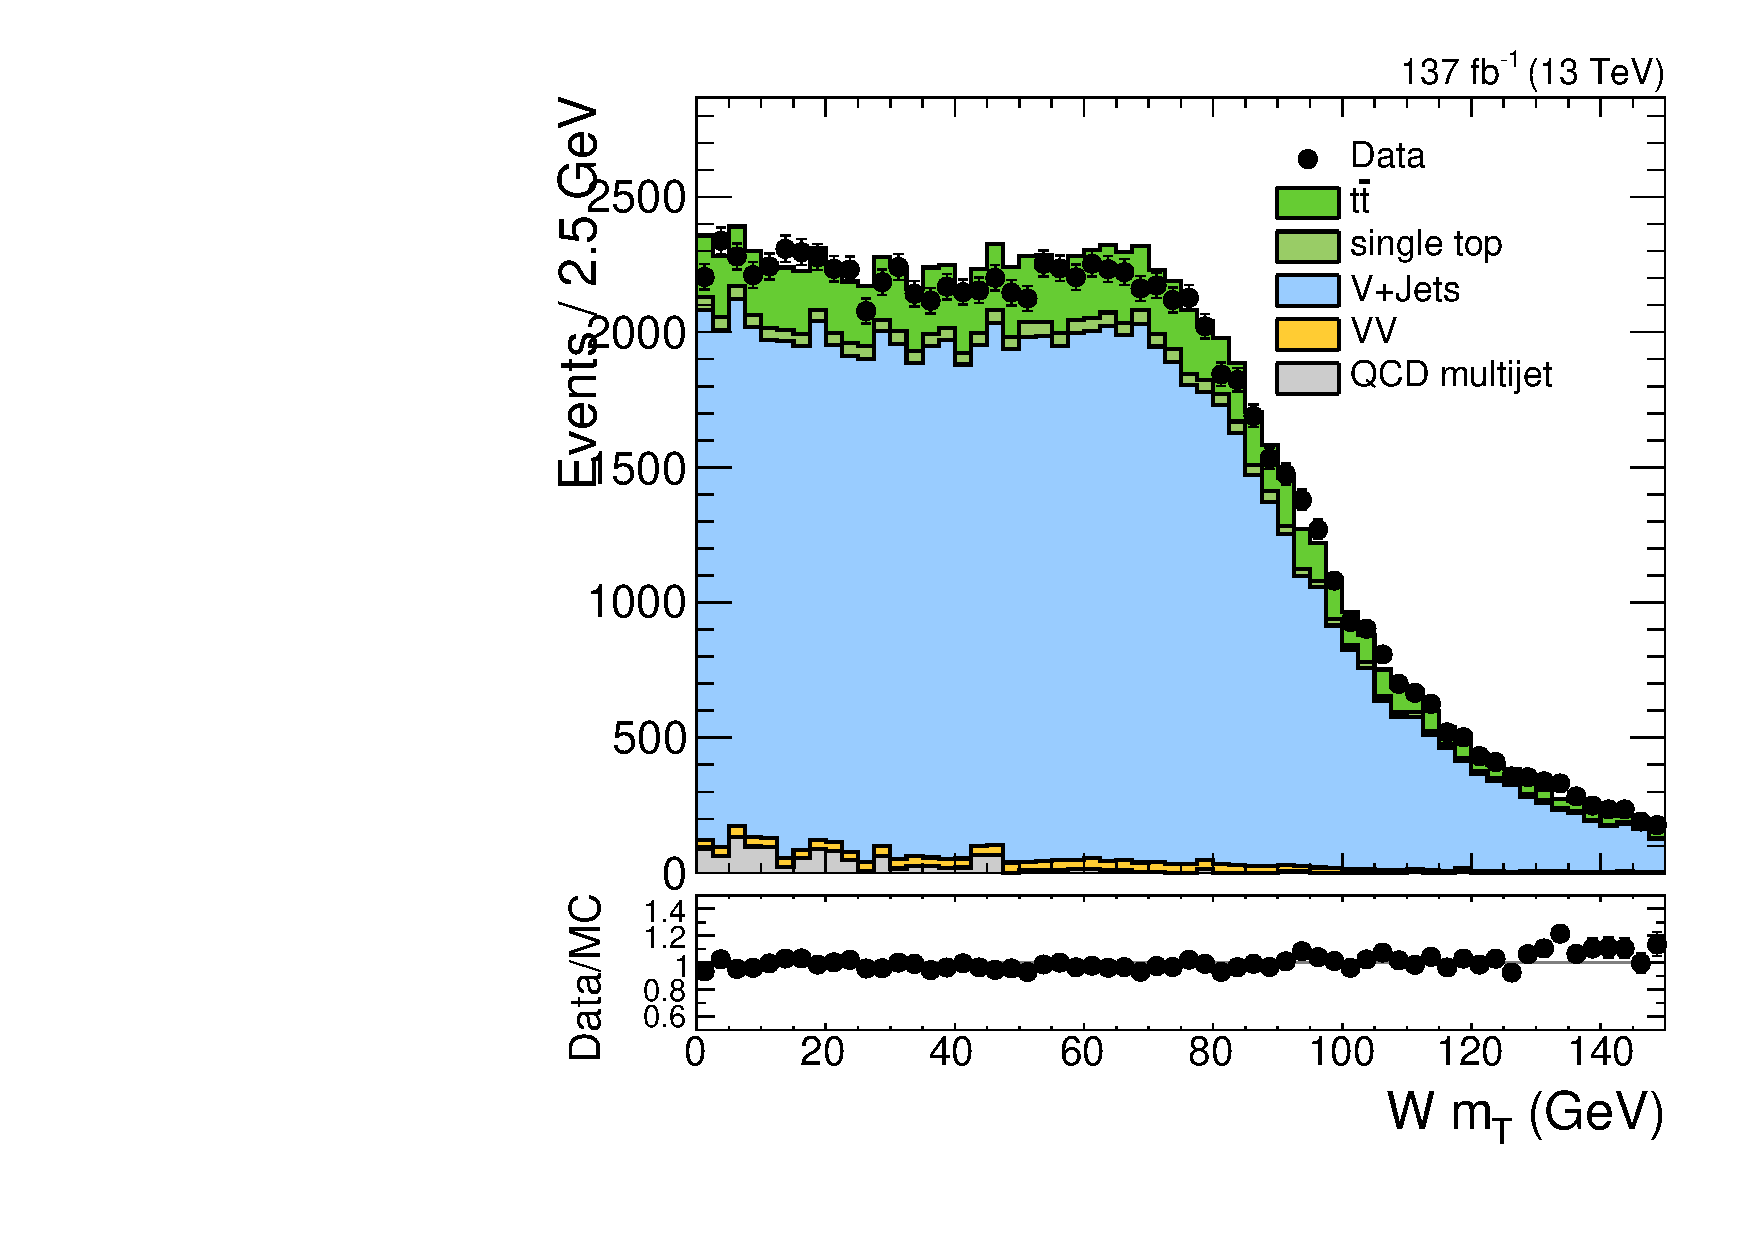
\includegraphics[width=0.3825\textwidth]{fig/controlPlots/SB_b1_mu_allP_allC_allD_Run2_lnujj_l1_mt.pdf}
  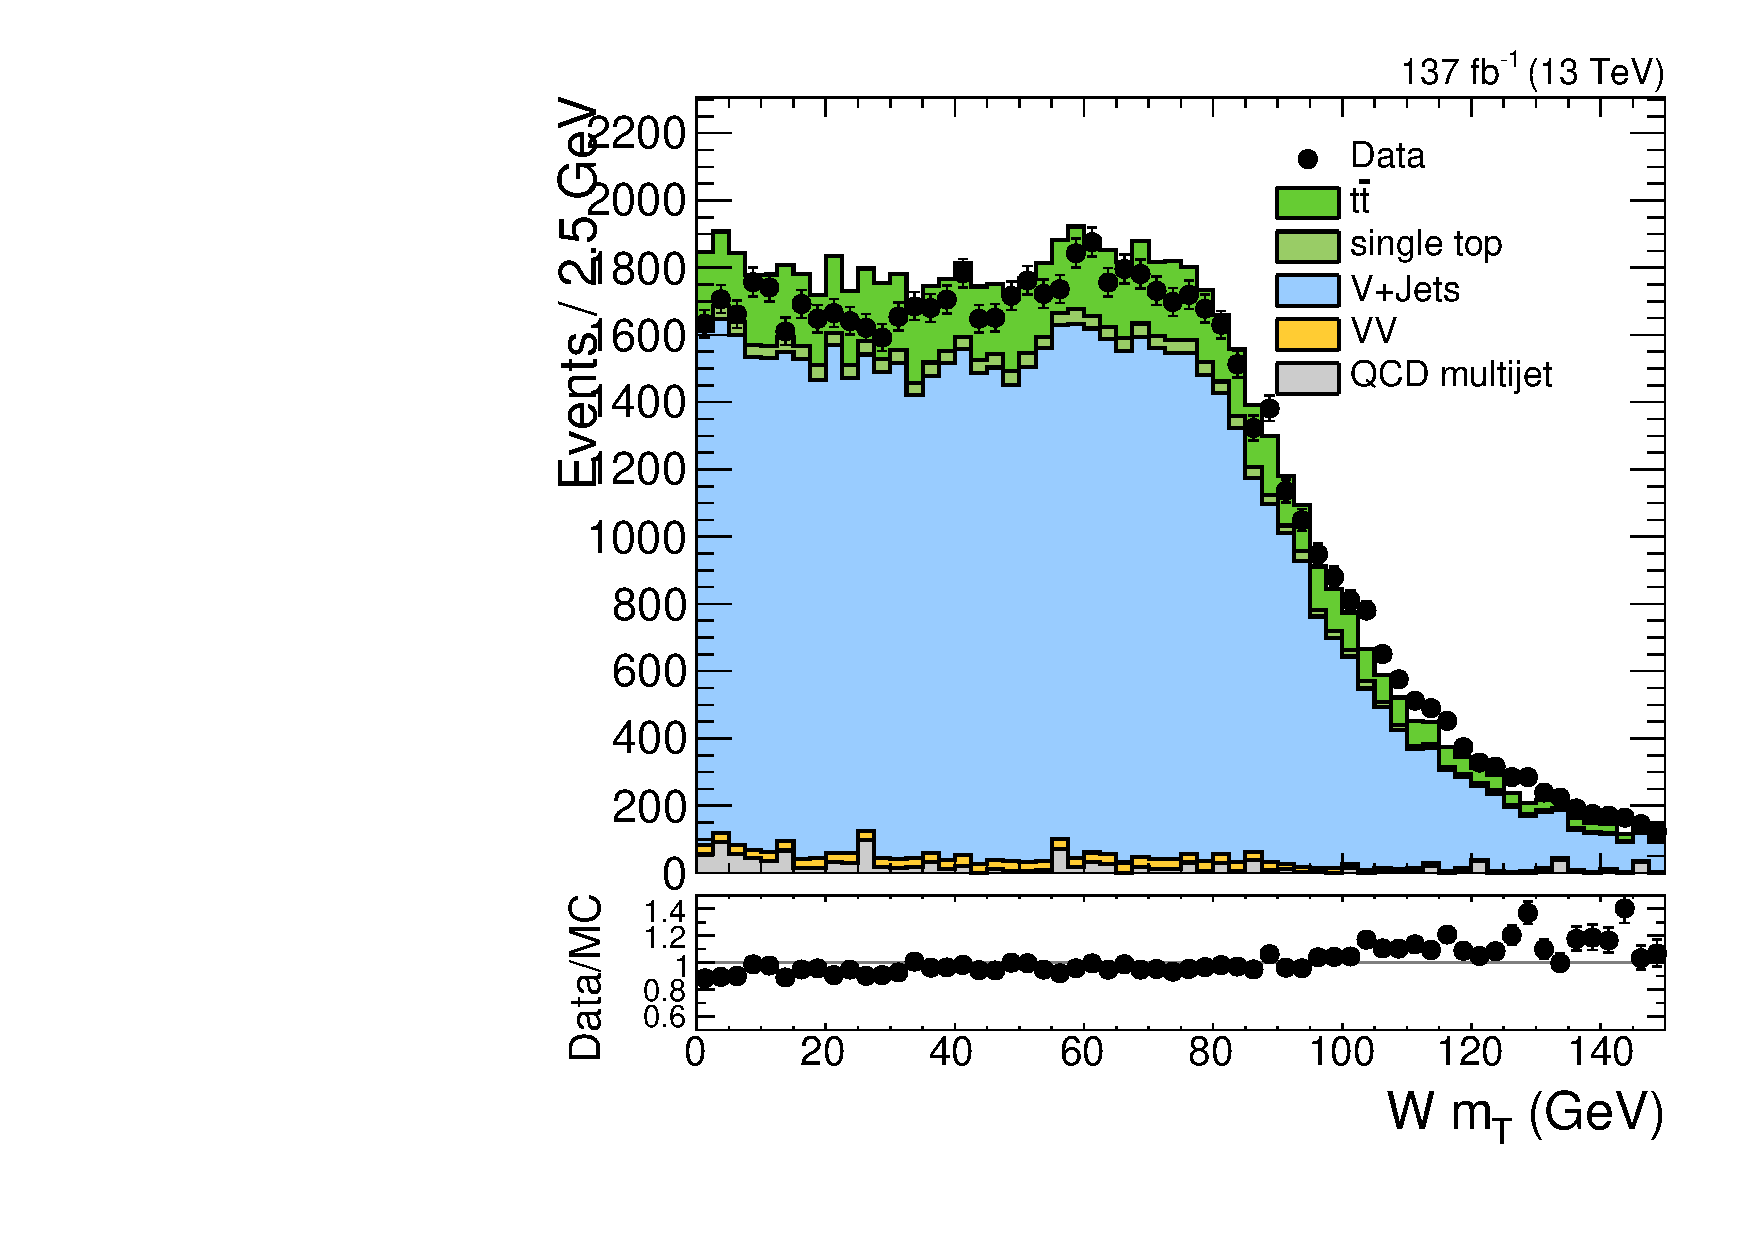
\includegraphics[width=0.3825\textwidth]{fig/controlPlots/SB_b1_e_allP_allC_allD_Run2_lnujj_l1_mt.pdf}\\
  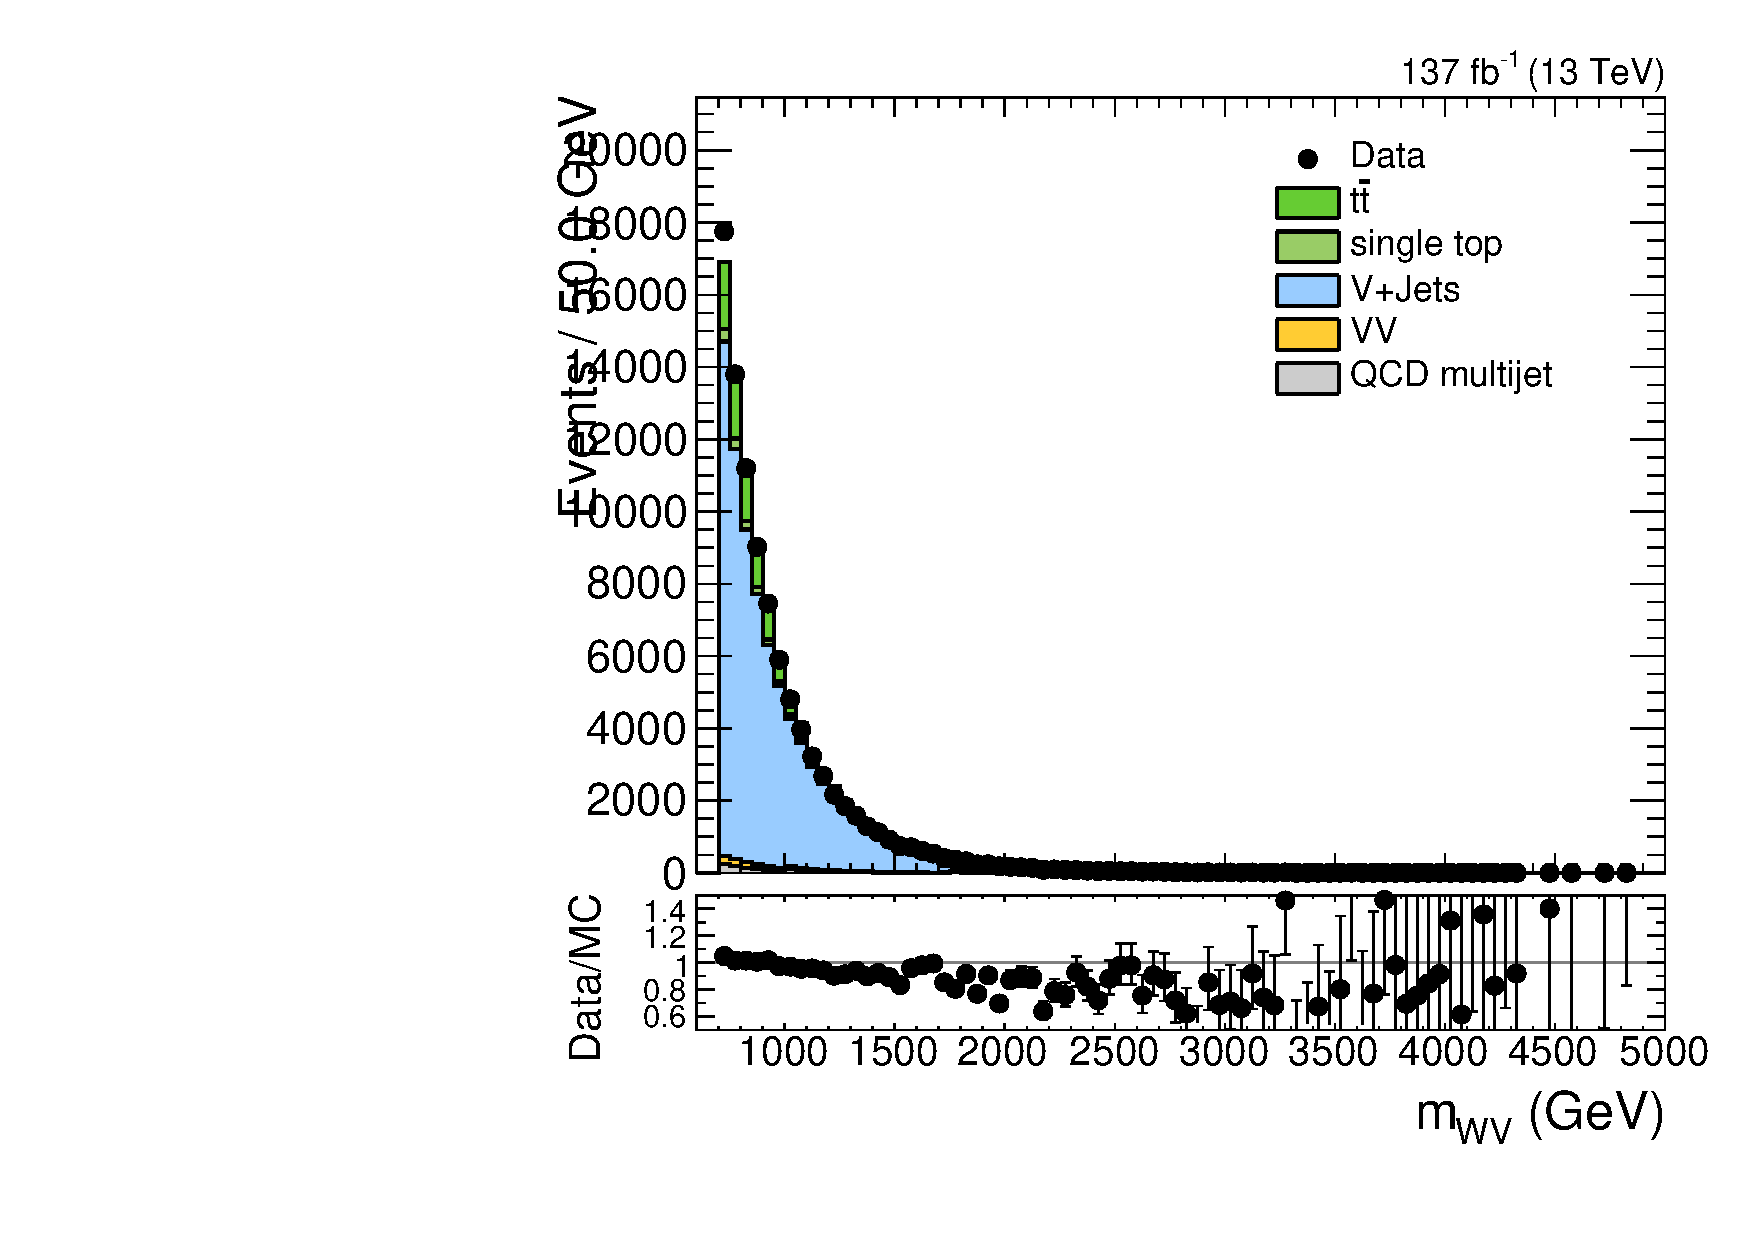
\includegraphics[width=0.3825\textwidth]{fig/controlPlots/SB_b1_mu_allP_allC_allD_Run2_mWV.pdf}
  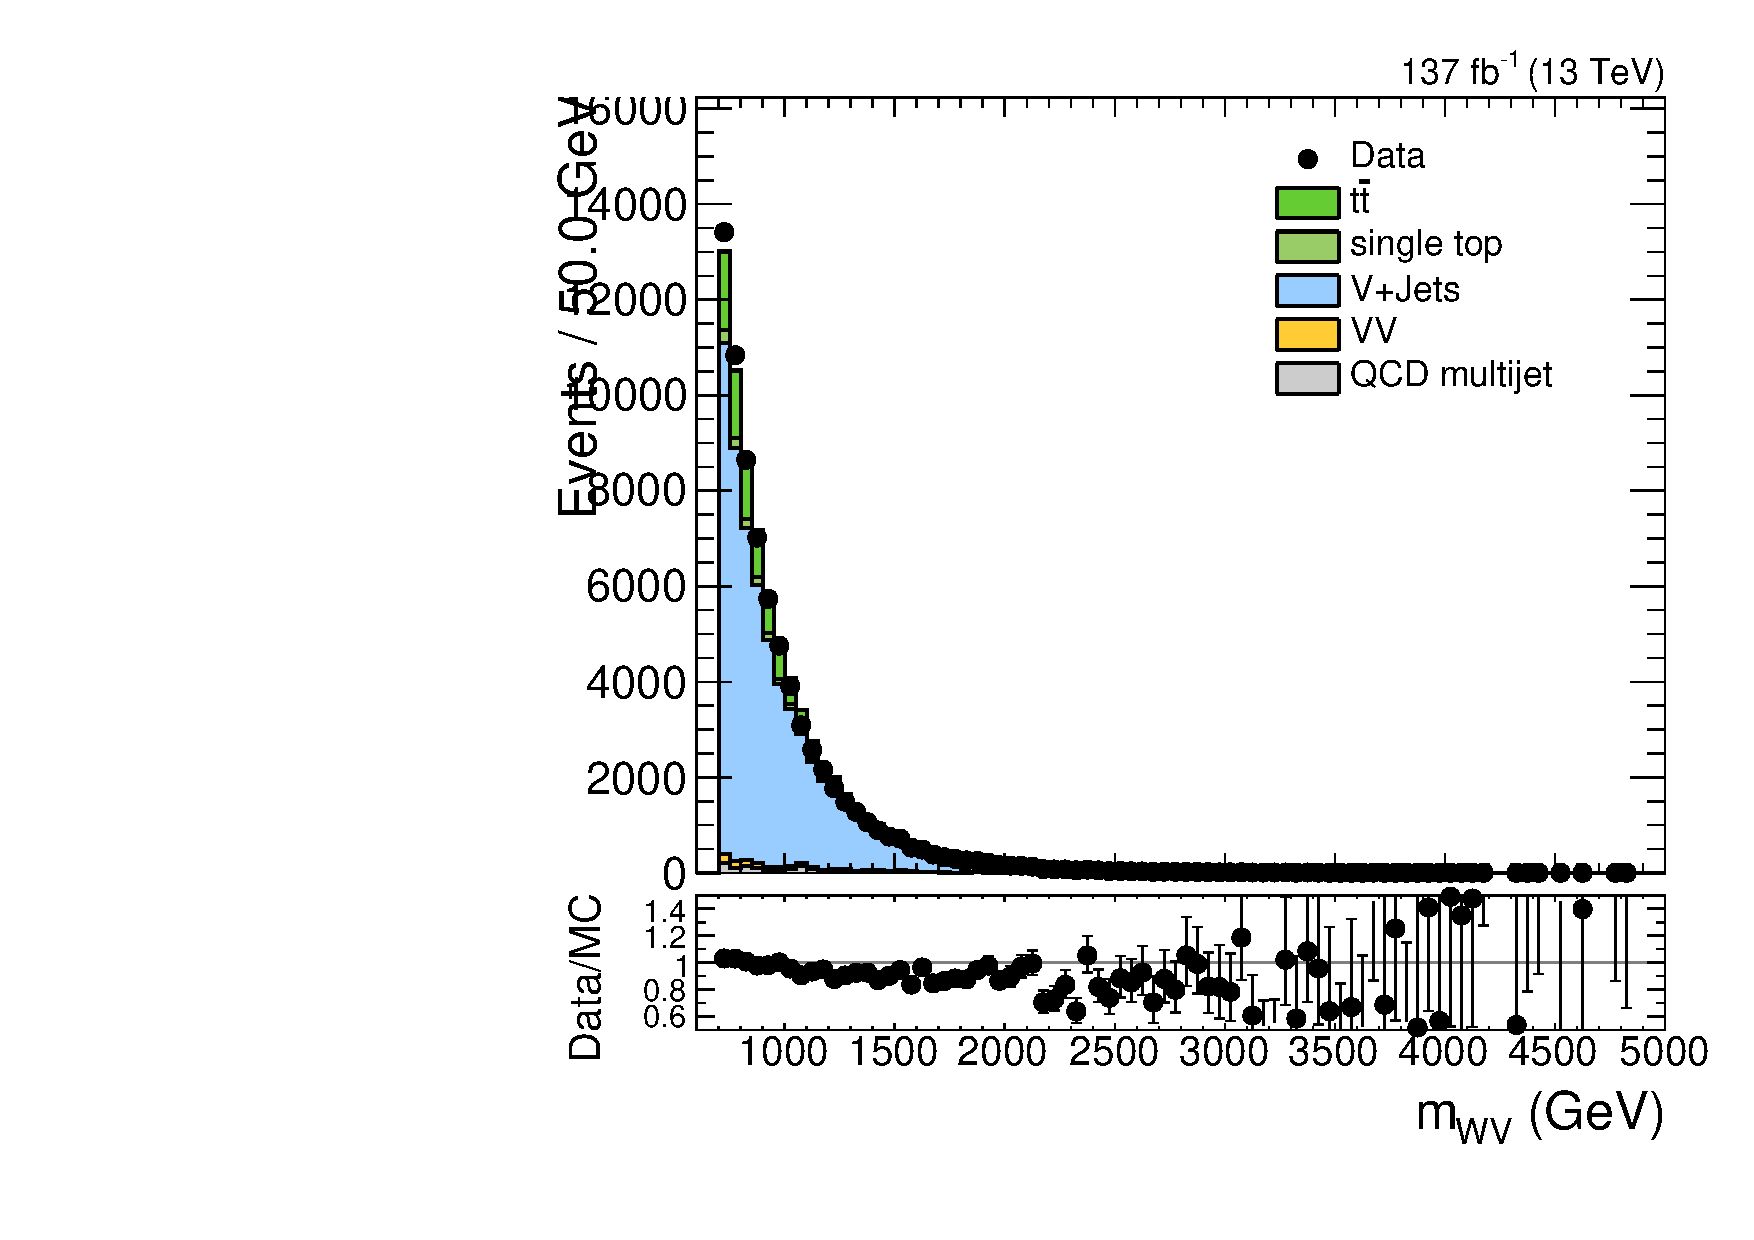
\includegraphics[width=0.3825\textwidth]{fig/controlPlots/SB_b1_e_allP_allC_allD_Run2_mWV.pdf}\\
  \caption{
    Comparison plots between data and MC from Run 2 for different \Wlep-related observables, in the jet mass sideband.
    From top to bottom: \pt of the leptonic $W$, transverse mass of the leptonic $W$, diboson invariant mass.
    Left: muon channel, right: electron channel.
  }
  \label{fig:SB_controlPlotsRun2_2}
\end{figure}

\begin{figure}[htbp]
  \centering
  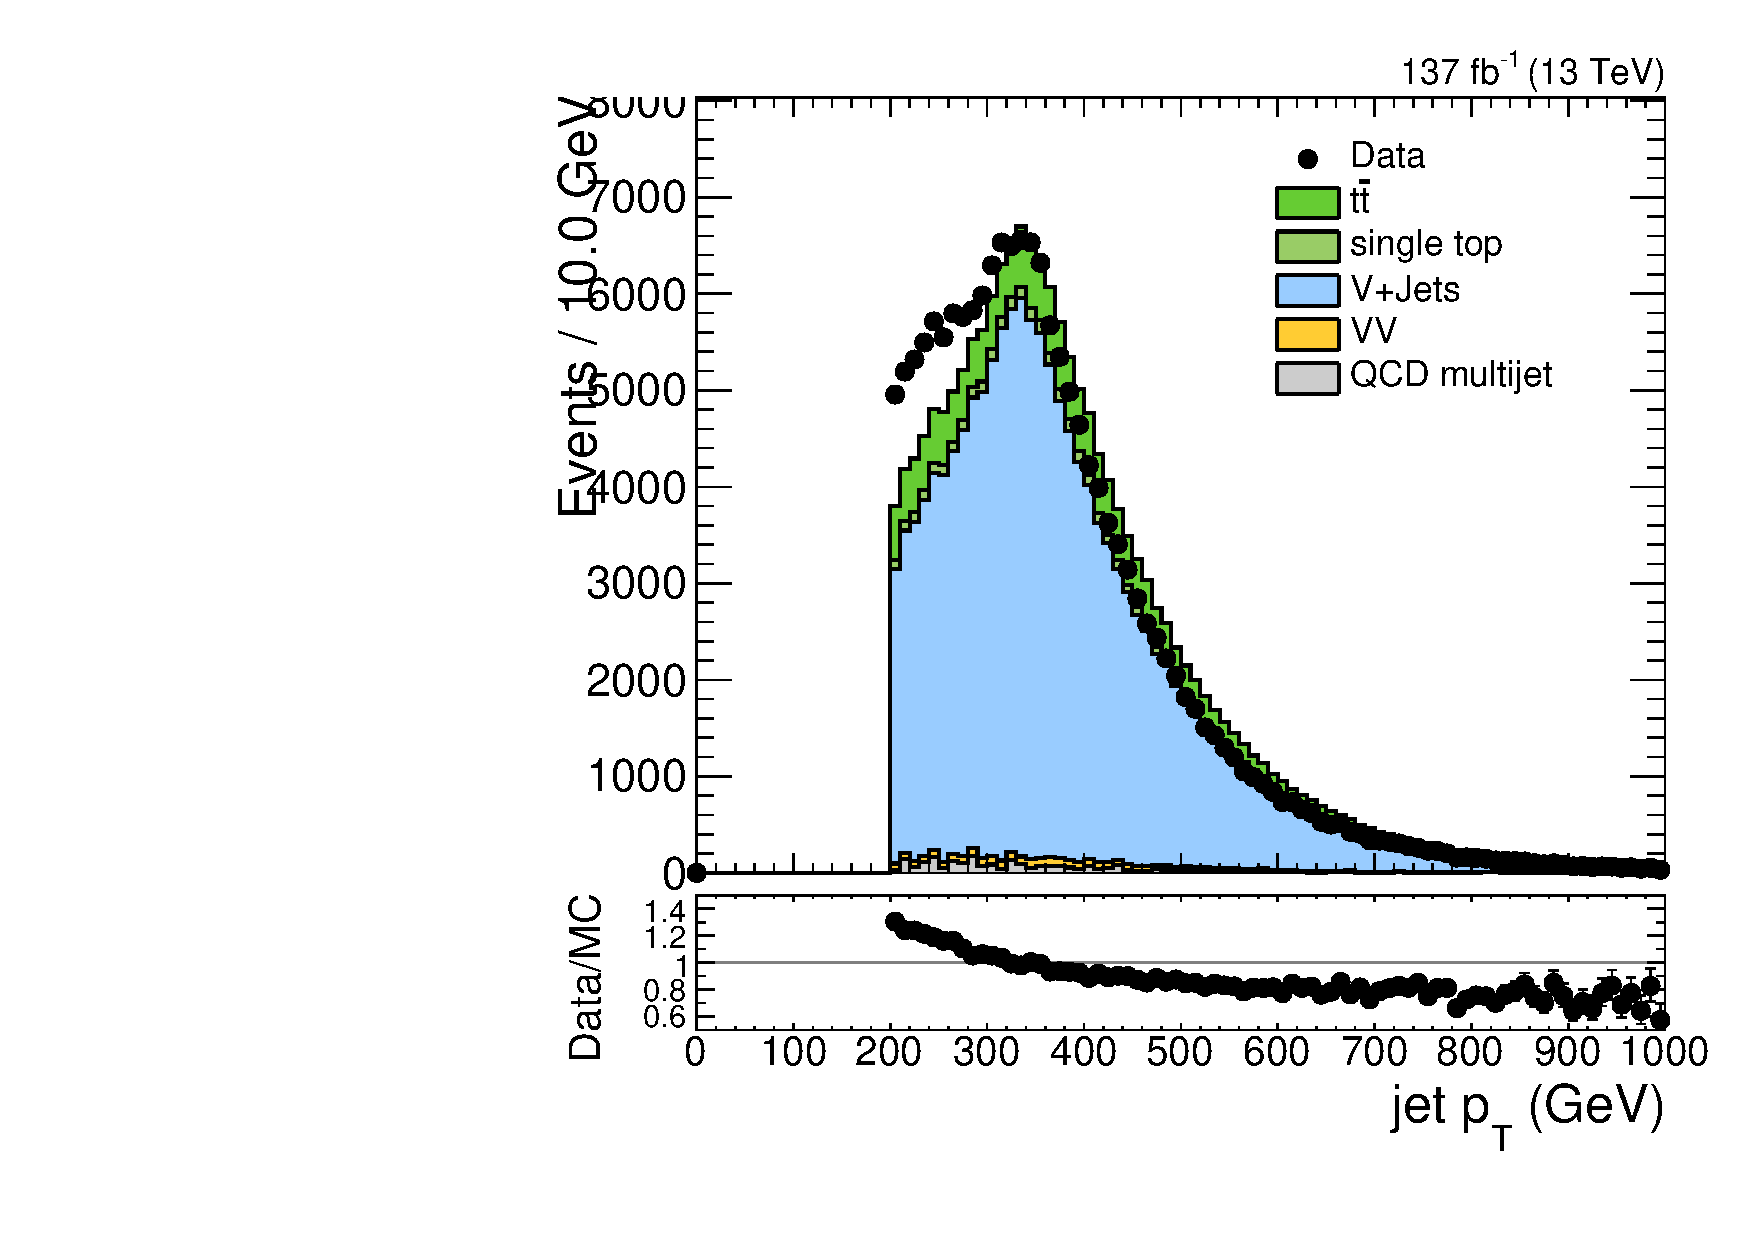
\includegraphics[width=0.3825\textwidth]{fig/controlPlots/SB_b1_allL_allP_allC_allD_Run2_lnujj_l2_pt.pdf}
  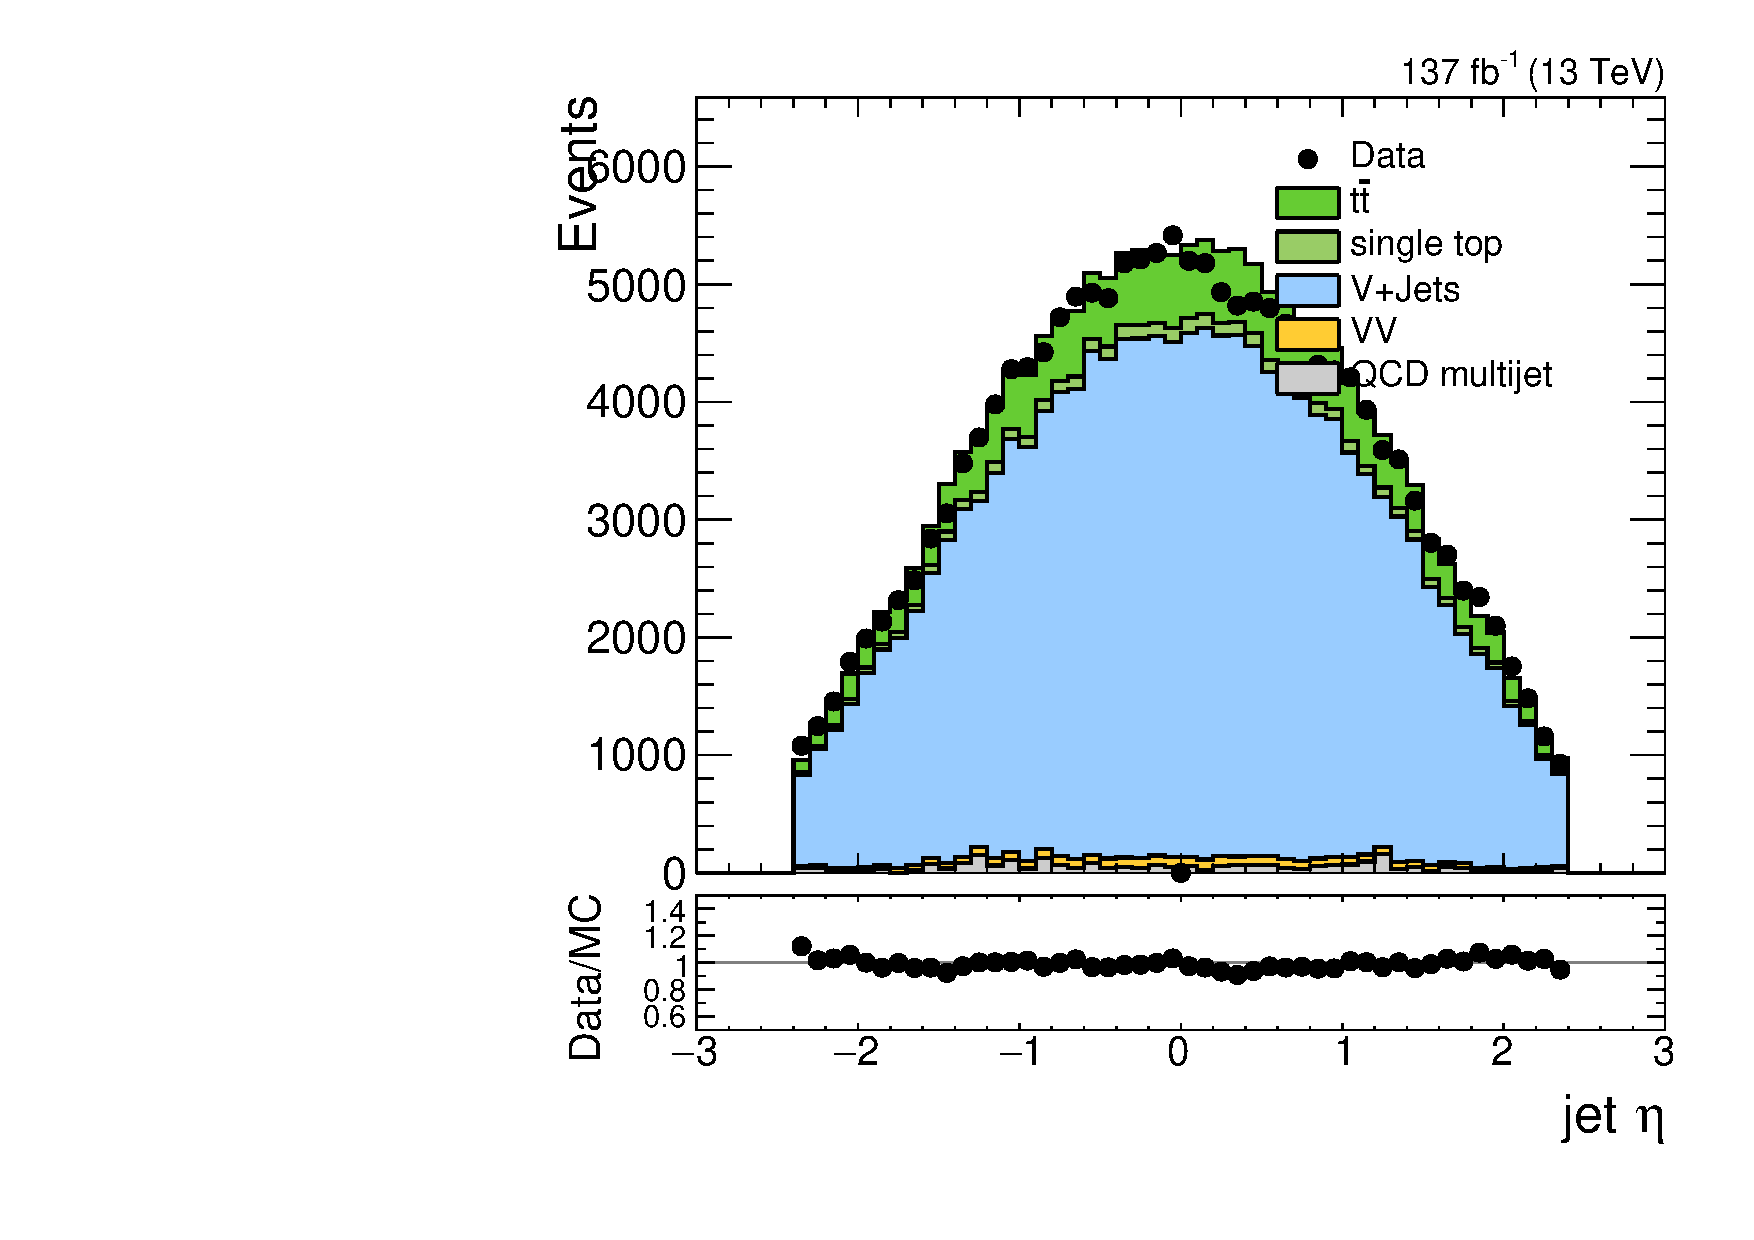
\includegraphics[width=0.3825\textwidth]{fig/controlPlots/SB_b1_allL_allP_allC_allD_Run2_lnujj_l2_eta.pdf}\\
  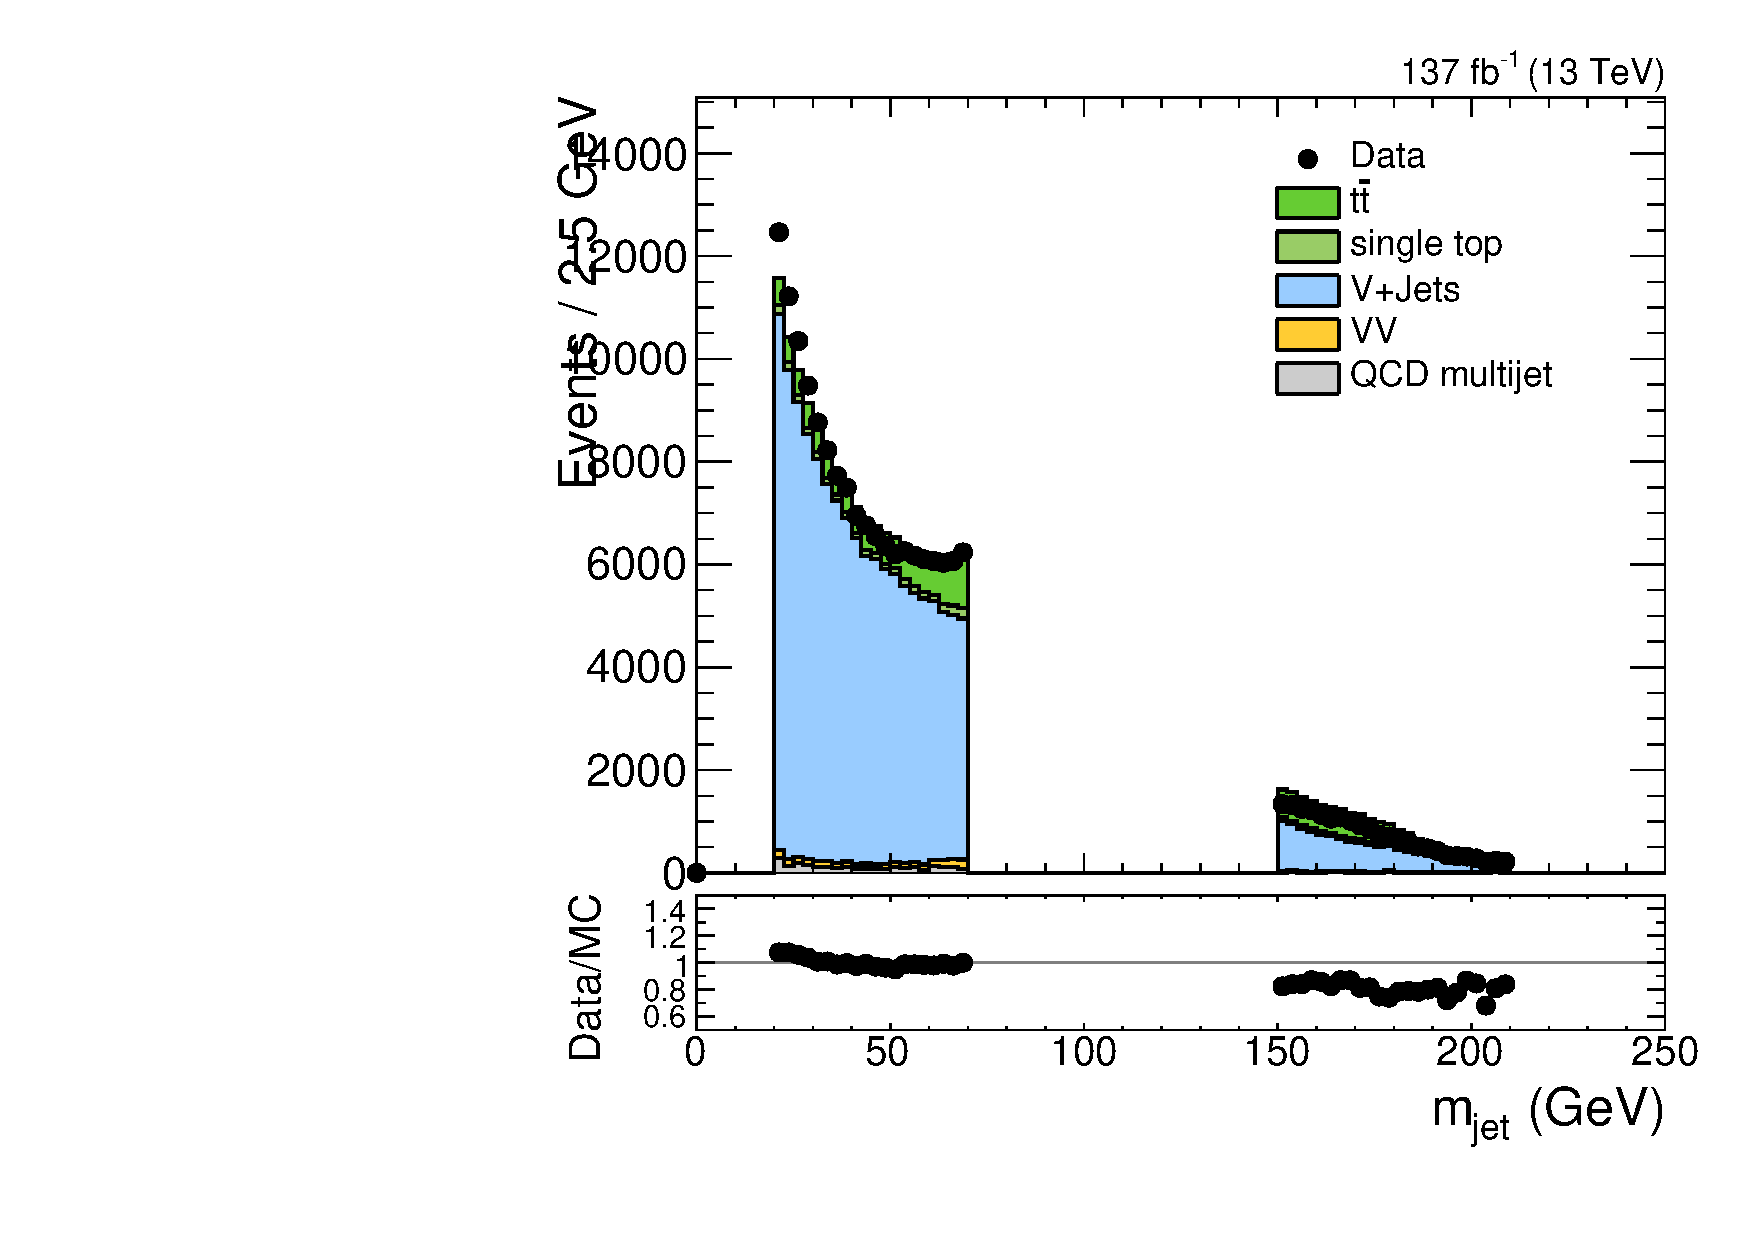
\includegraphics[width=0.3825\textwidth]{fig/controlPlots/SB_b1_allL_allP_allC_allD_Run2_mjet.pdf}\\
  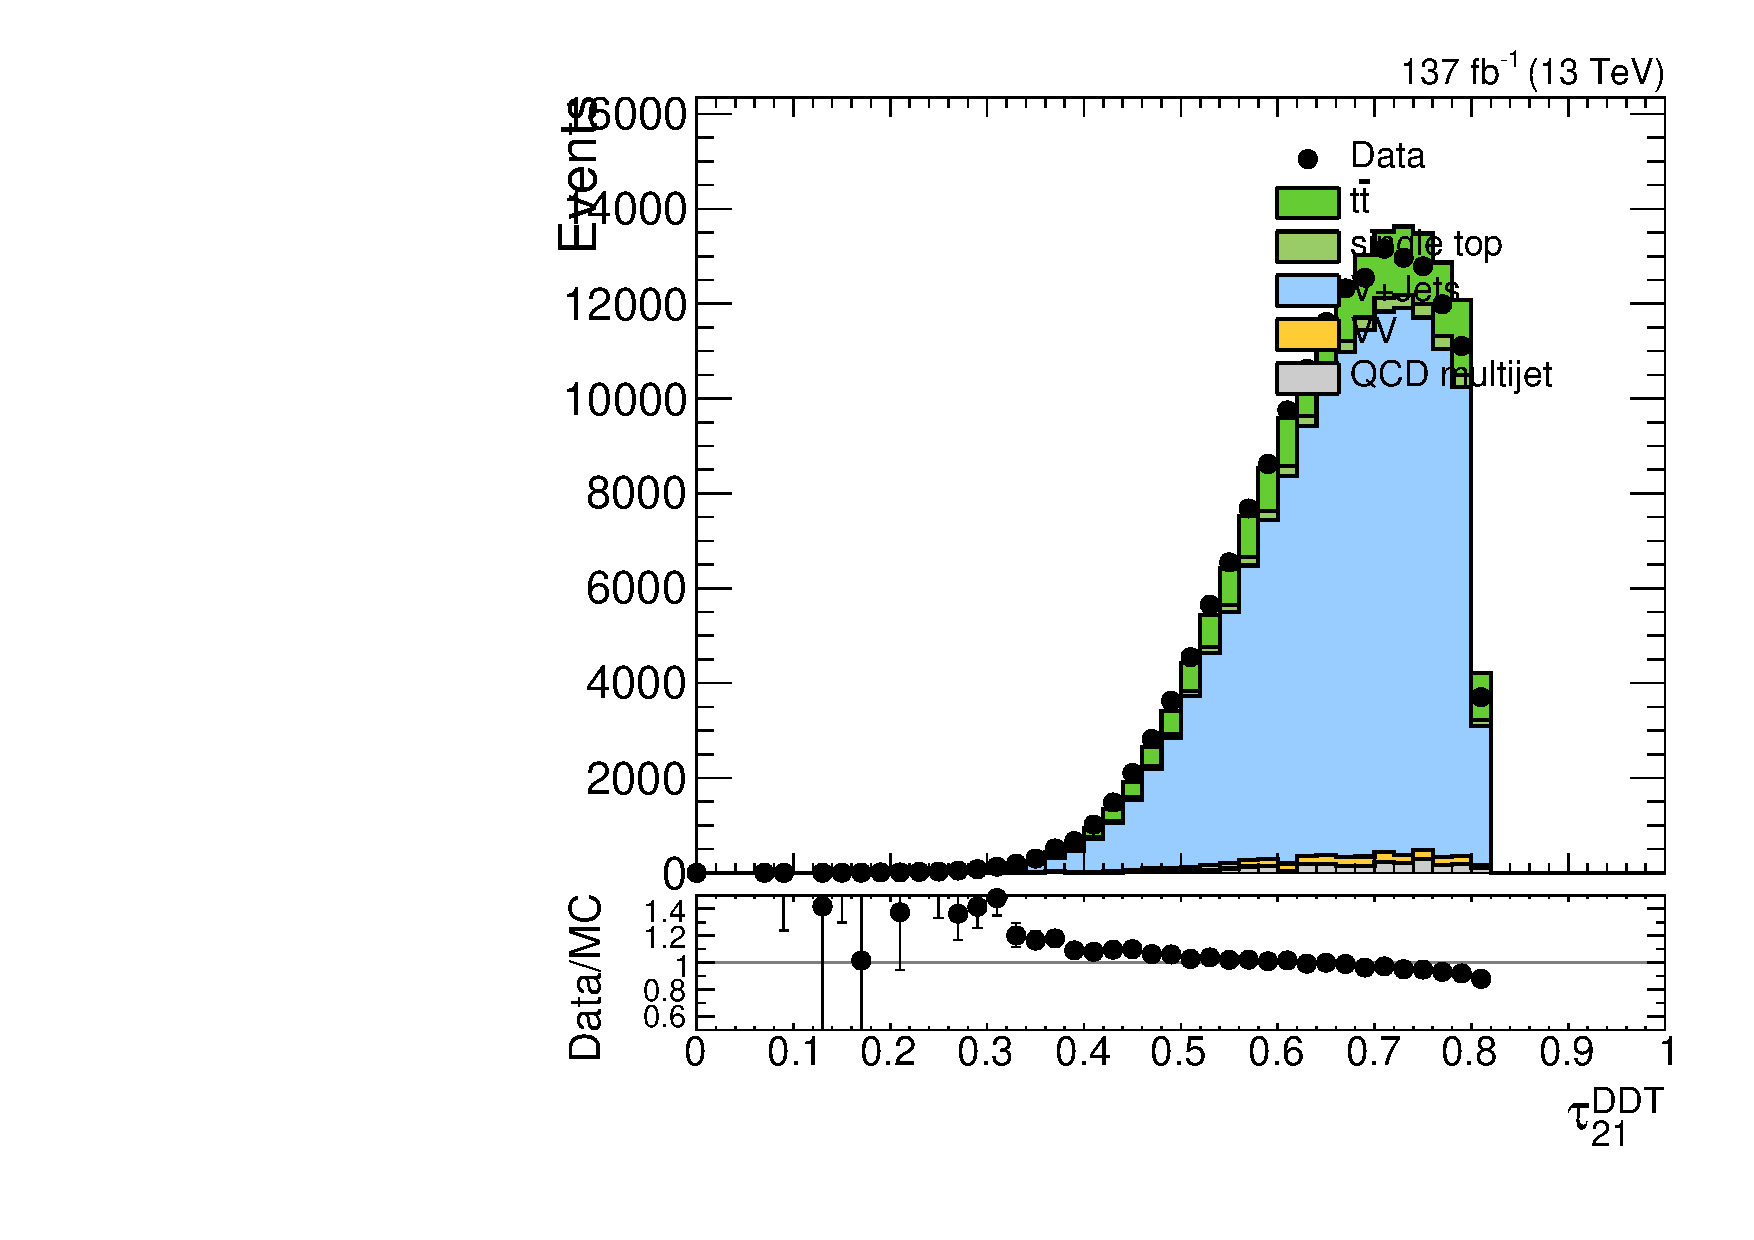
\includegraphics[width=0.3825\textwidth]{fig/controlPlots/SB_b1_allL_allP_allC_allD_Run2_tau21DDT.pdf}
  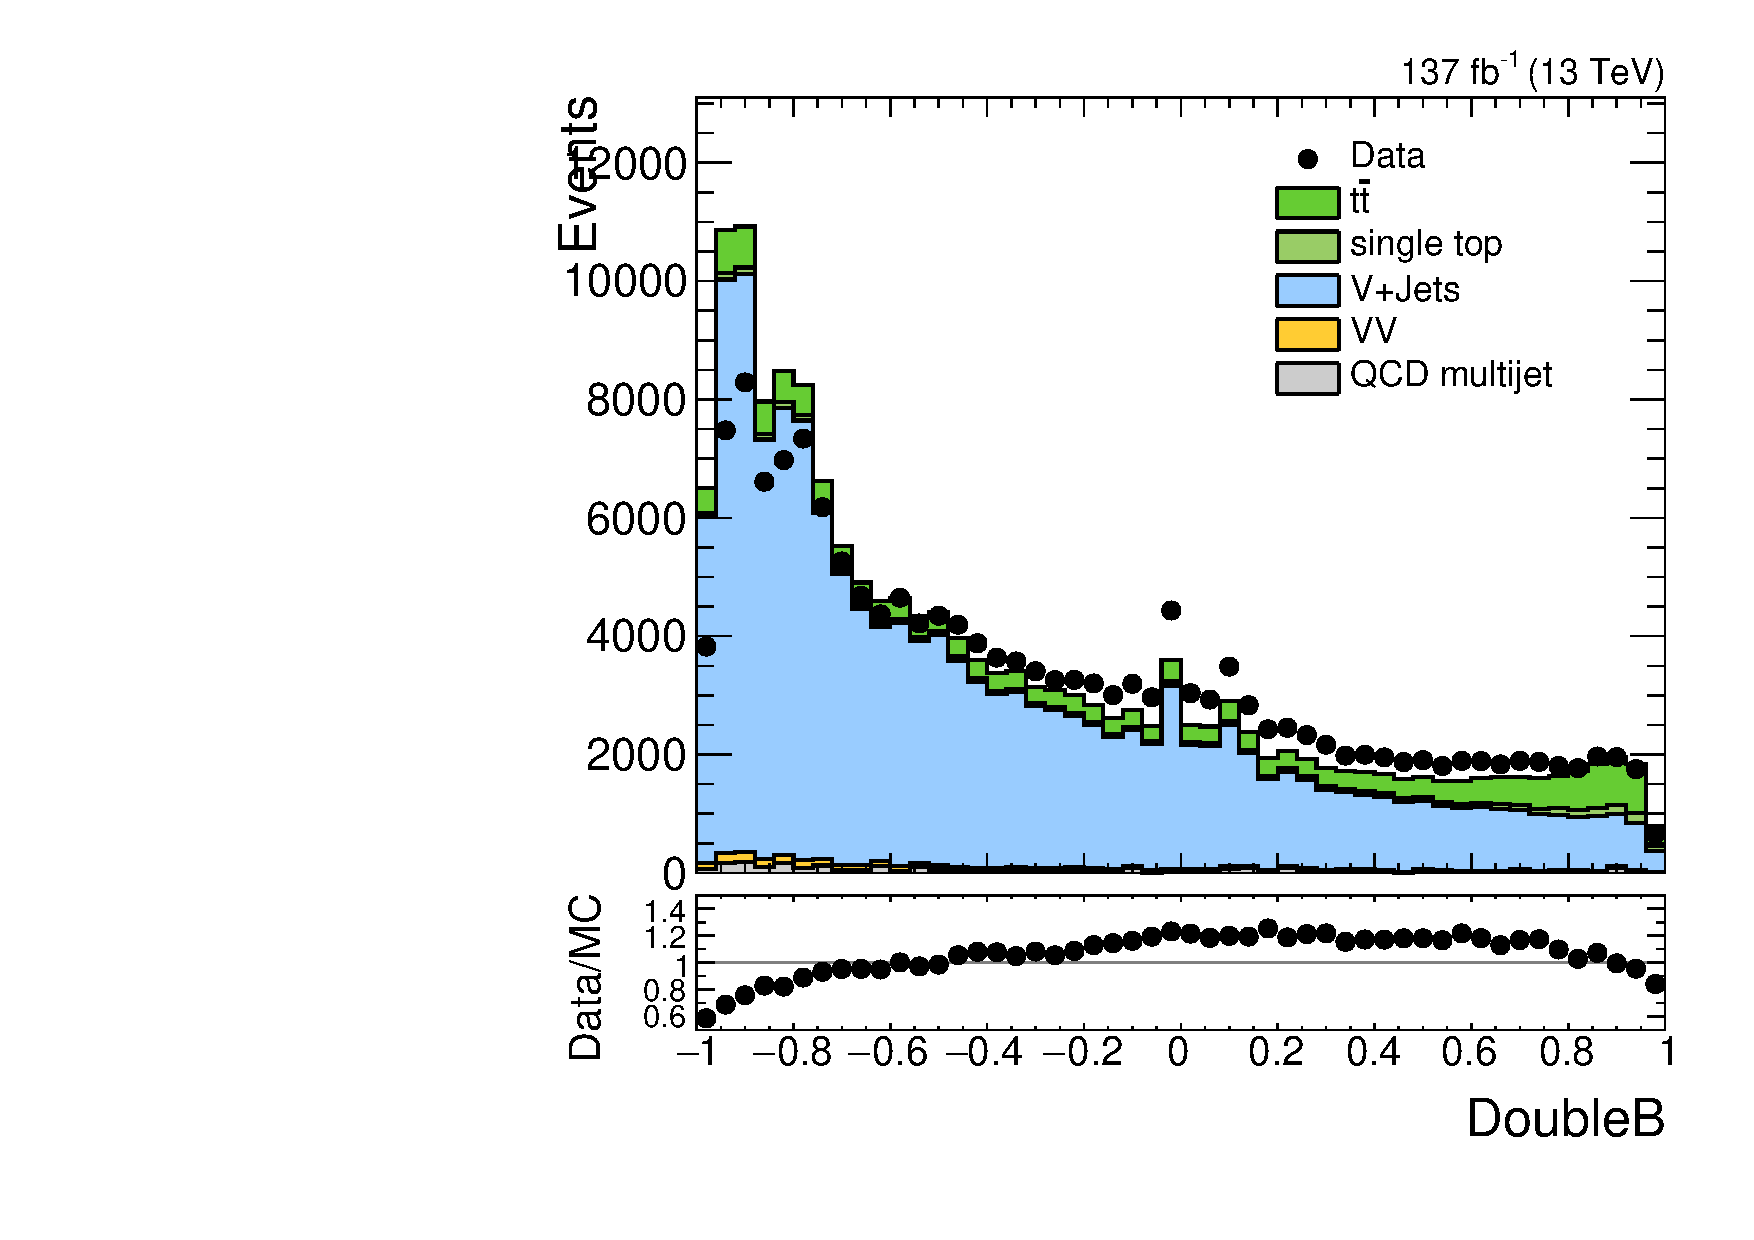
\includegraphics[width=0.3825\textwidth]{fig/controlPlots/SB_b1_allL_allP_allC_allD_Run2_DoubleB.pdf}\\
  \caption{
    Comparison plots between data and MC from Run 2 for the \pt, $\eta$, \MJ (soft drop mass), \nsubjDDT, and \DoubleB tagger of the selected \Vhad candidate (leading AK8 jet), in the jet mass sideband.
  }
  \label{fig:SB_controlPlotsRun2_3}
\end{figure}

\begin{figure}[htbp]
  \centering
  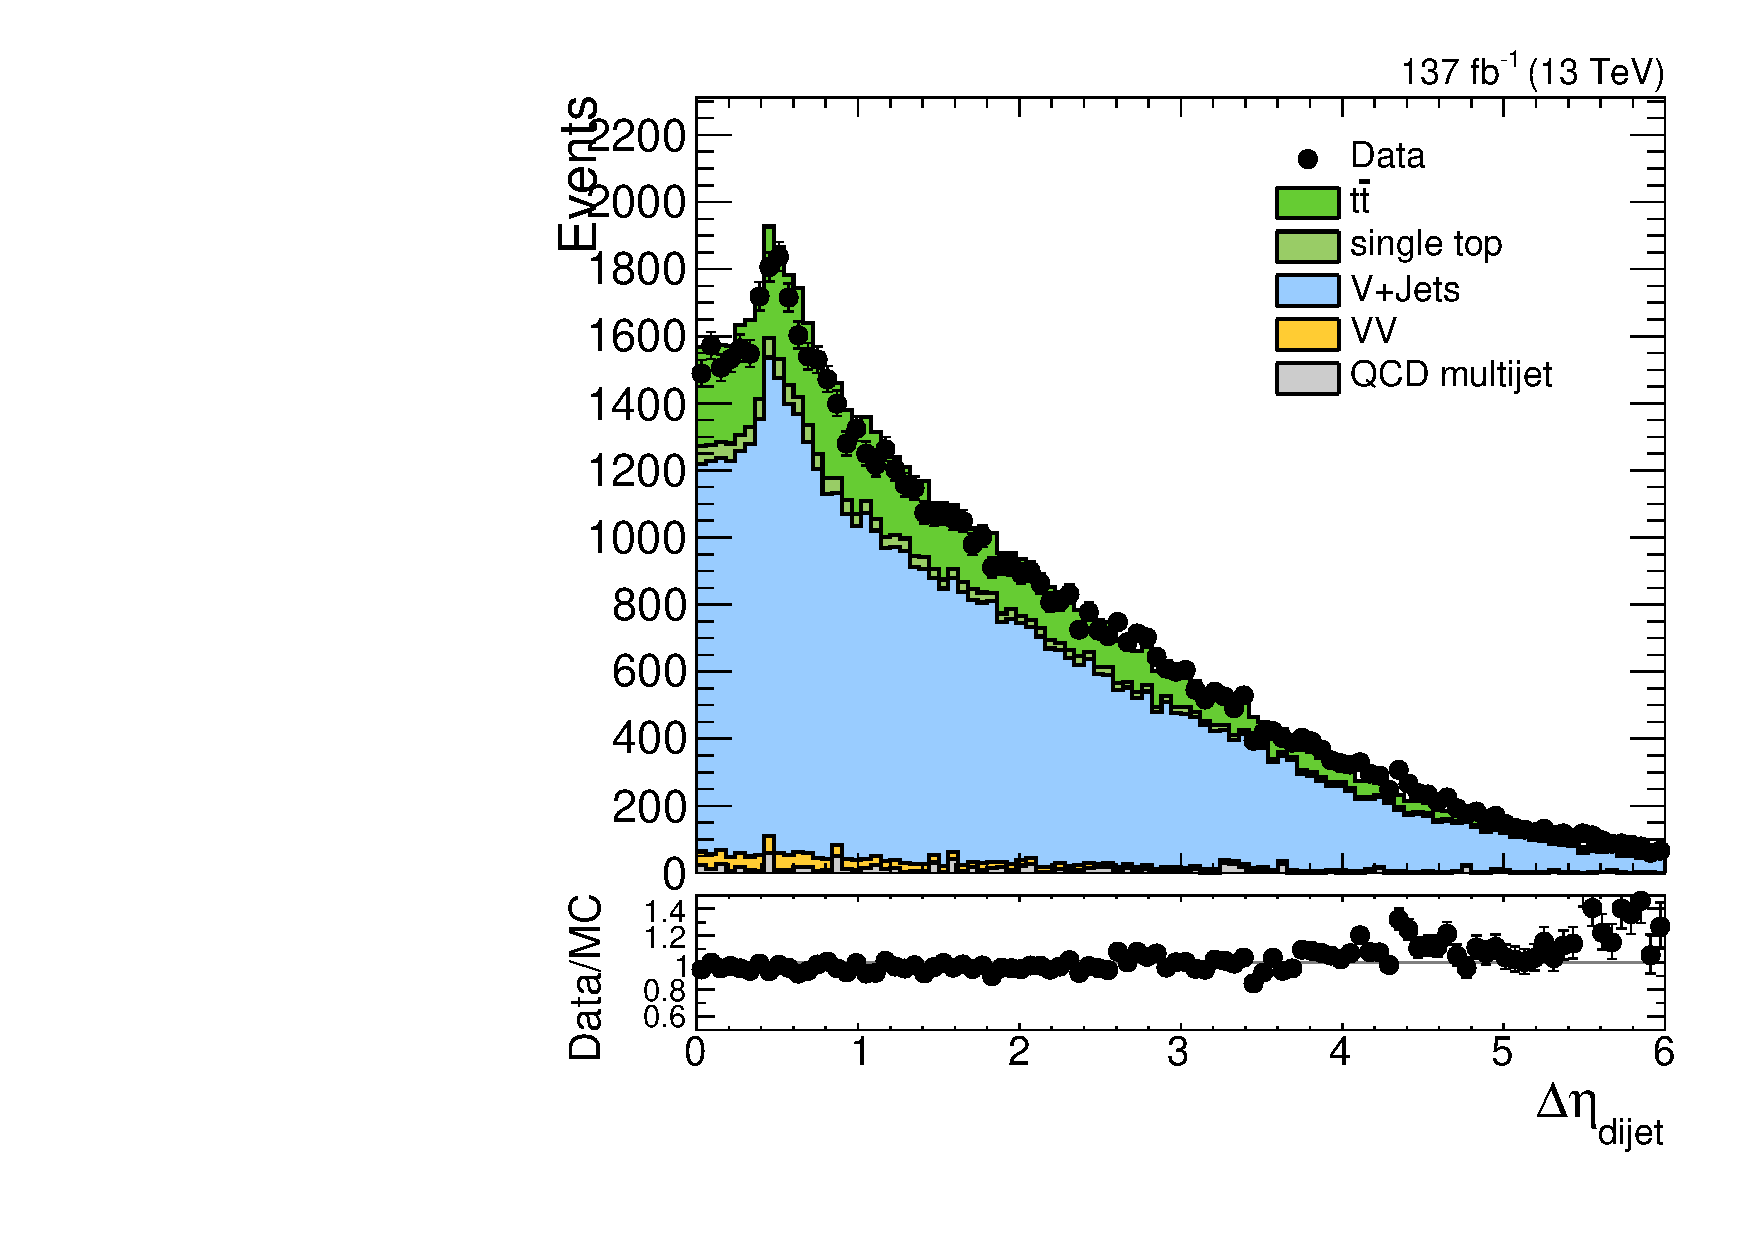
\includegraphics[width=0.3825\textwidth]{fig/controlPlots/SB_b1_allL_allP_allC_allD_Run2_lnujj_vbfDEta.pdf}
  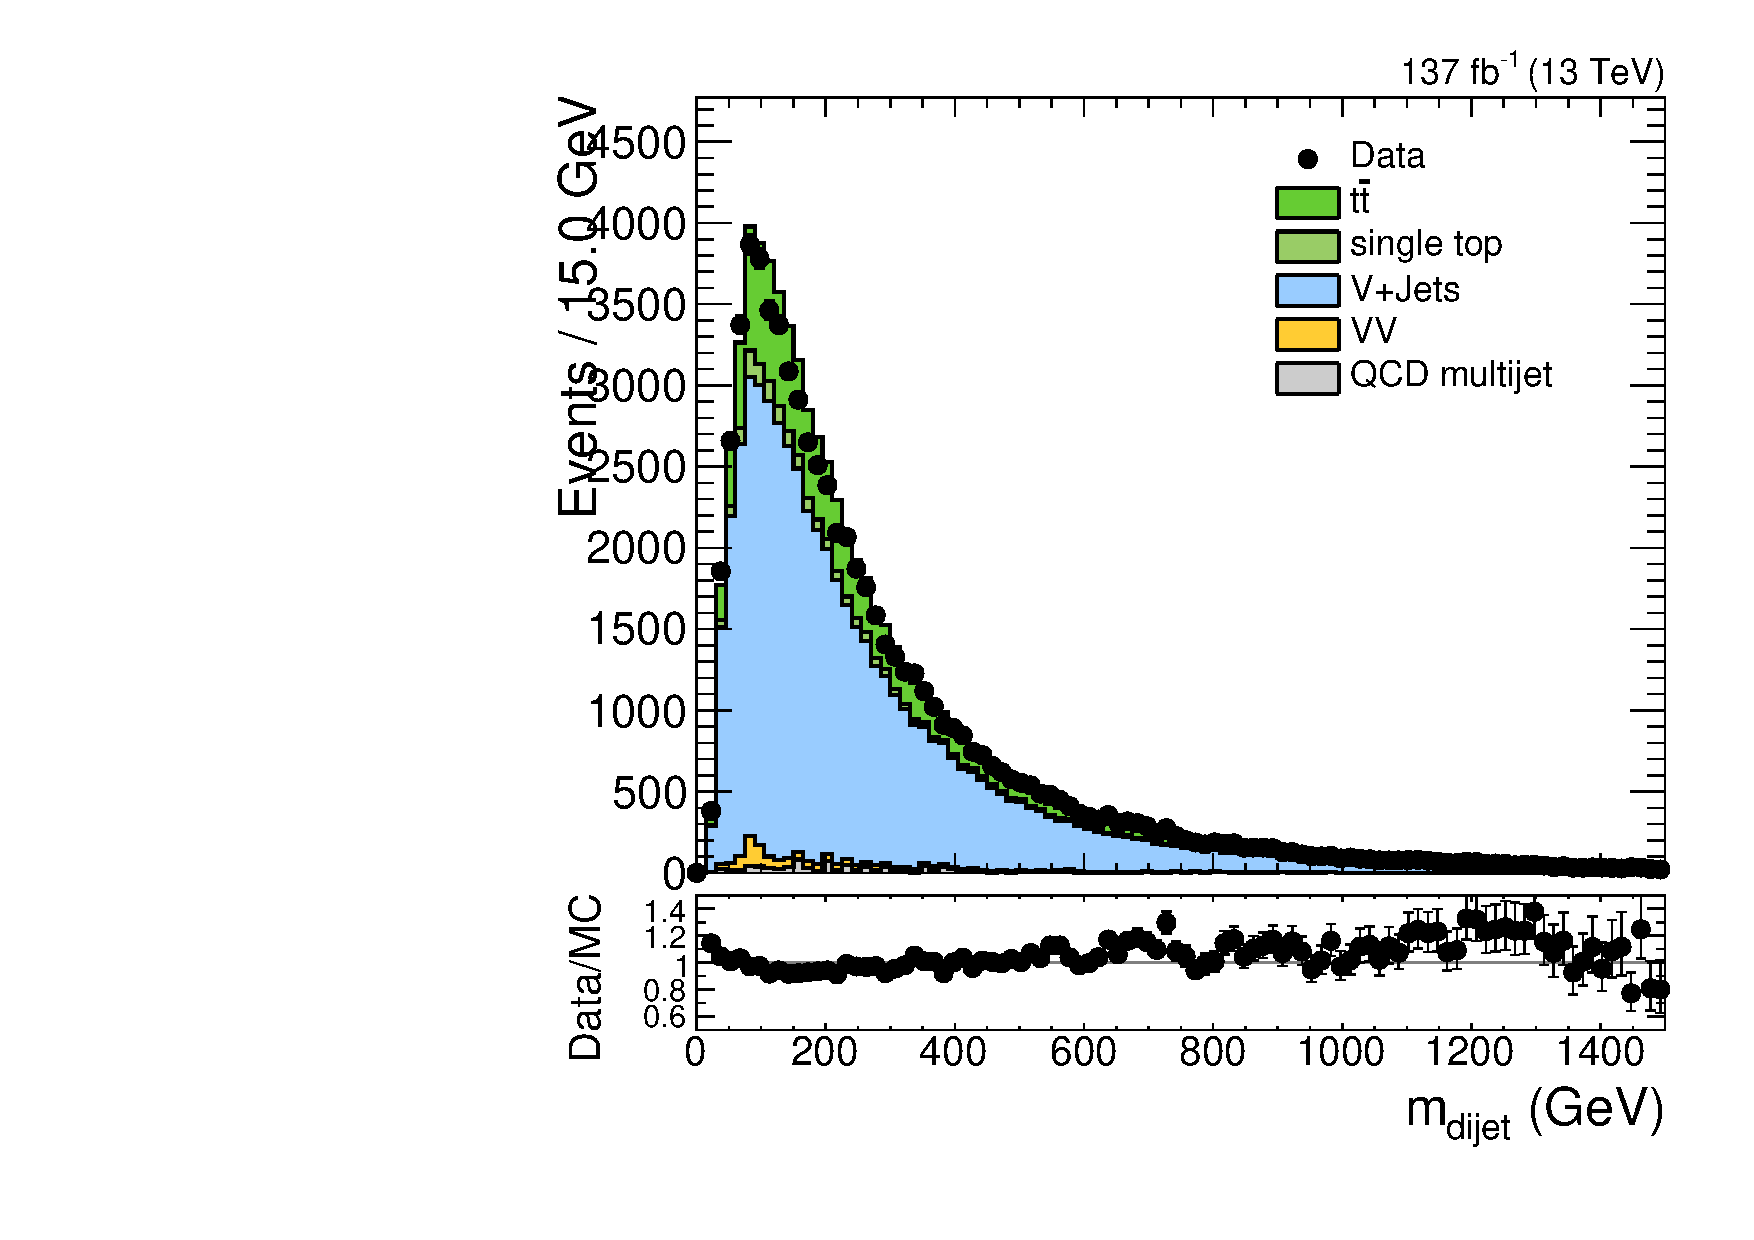
\includegraphics[width=0.3825\textwidth]{fig/controlPlots/SB_b1_allL_allP_allC_allD_Run2_lnujj_vbfMass.pdf}\\
  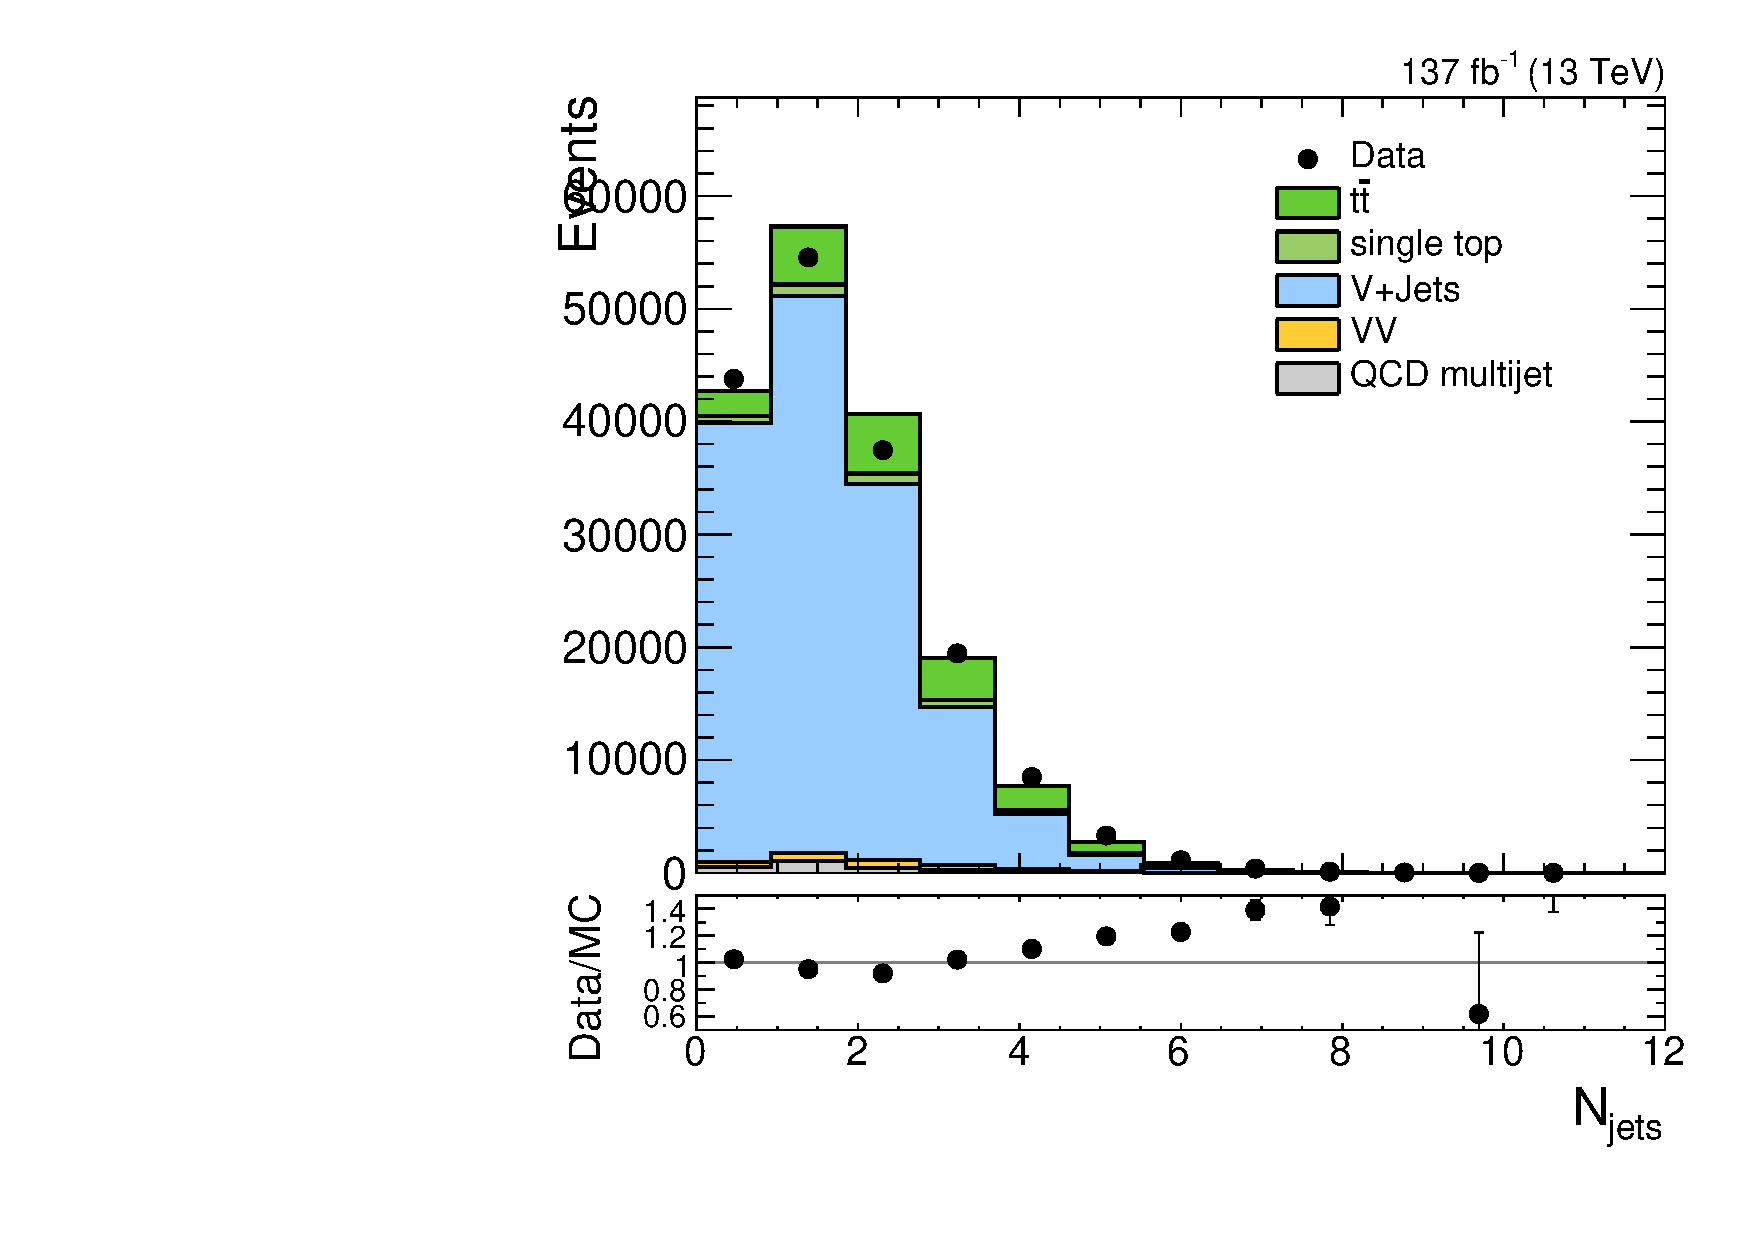
\includegraphics[width=0.3825\textwidth]{fig/controlPlots/SB_b1_allL_allP_allC_allD_Run2_lnujj_nJets.pdf}
  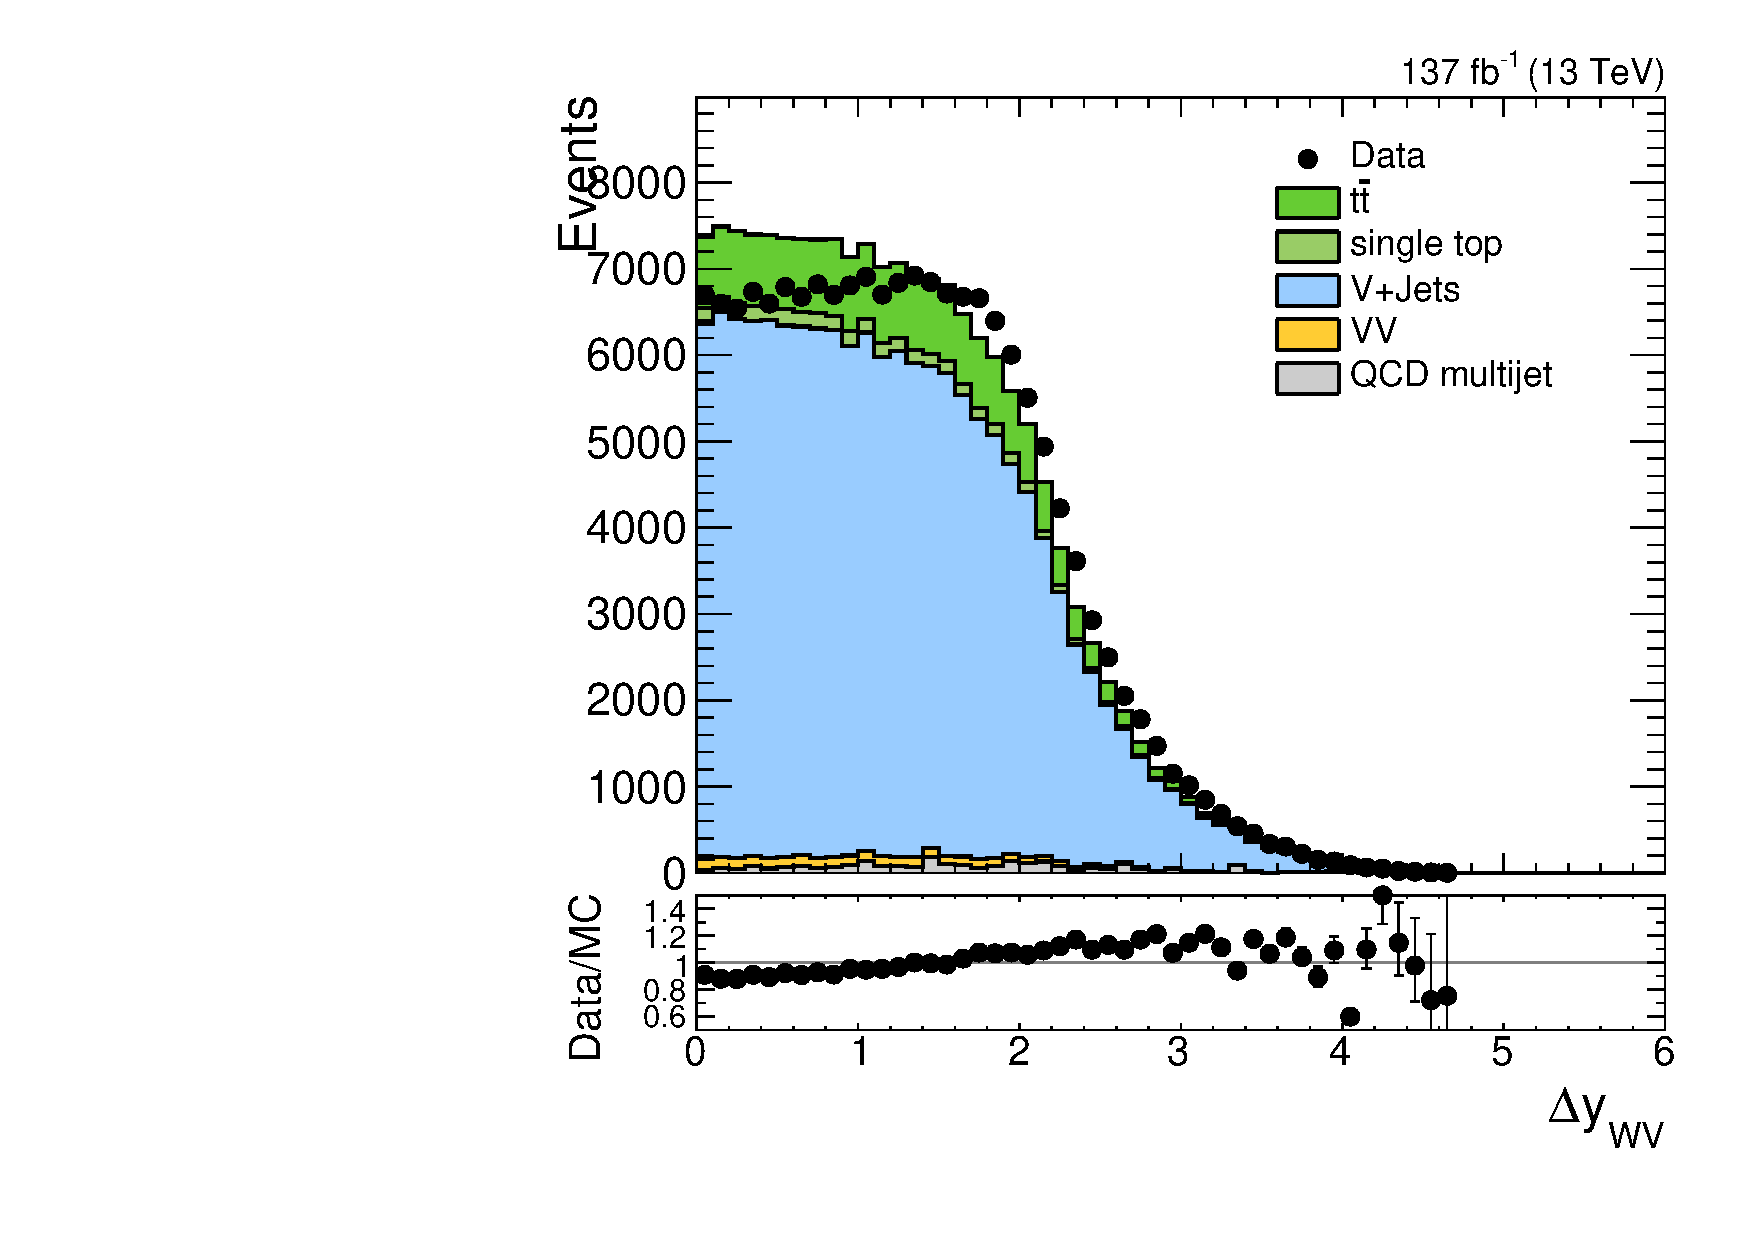
\includegraphics[width=0.3825\textwidth]{fig/controlPlots/SB_b1_allL_allP_allC_allD_Run2_dy.pdf}\\
  \caption{
    Comparison plots between data and MC from Run 2 for the separation in $\eta$ of the \VBF forward jets, invariant mass of the \VBF jets, number of selected standard jets, and rapidity separation between the reconstructed bosons, in the jet mass sideband.
  }
  \label{fig:SB_controlPlotsRun2_4}
\end{figure}

\subsubsection{Control Plots in the Top-Enriched Control Region}

% Top-enriched control plots
Figure~\ref{fig:CR_controlPlotsRun2_1} shows control plots of lepton-related observables in the top-enriched control region, with the lepton \pt, $\eta$, and \ptmiss in both the $e$ and $\mu$ channels.
For figure~\ref{fig:CR_controlPlotsRun2_2}, the distributions of the \Wlep \pt, transverse mass, and \MVV are shown, for both the $e$ and $\mu$ channels.
In figure~\ref{fig:CR_controlPlotsRun2_3}, distributions of variables related to the \Vhad jet are shown, with the jet \pt, $\eta$, \MJ, \nsubjDDT, and \DoubleB tagger.
Finally, in figure~\ref{fig:CR_controlPlotsRun2_4}, \VBF-related distributions are shown for \DetaVBF, \mjjVBF, \nJets, and \Dy.

\begin{figure}[htbp]
  \centering
  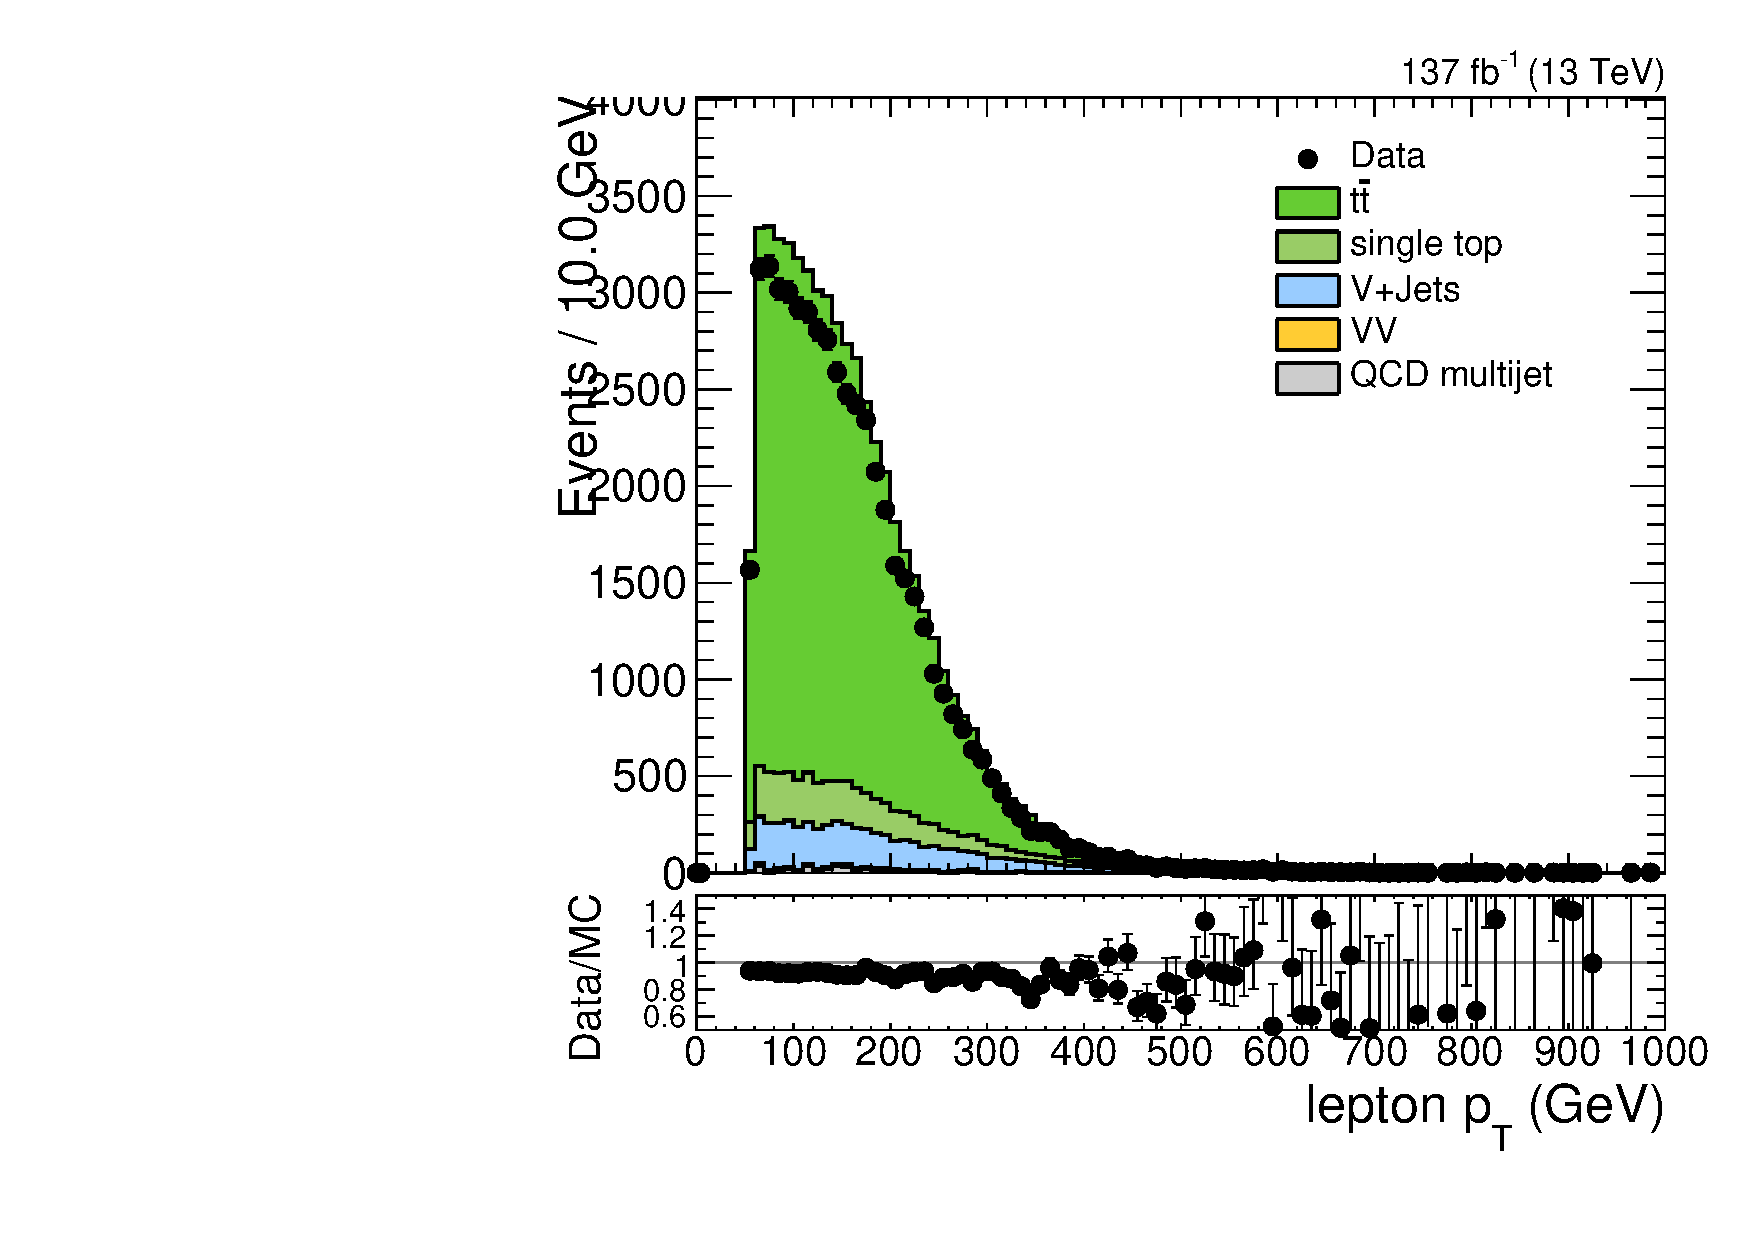
\includegraphics[width=0.3825\textwidth]{fig/controlPlots/CR_b1_mu_allP_allC_allD_Run2_lnujj_l1_l_pt.pdf}
  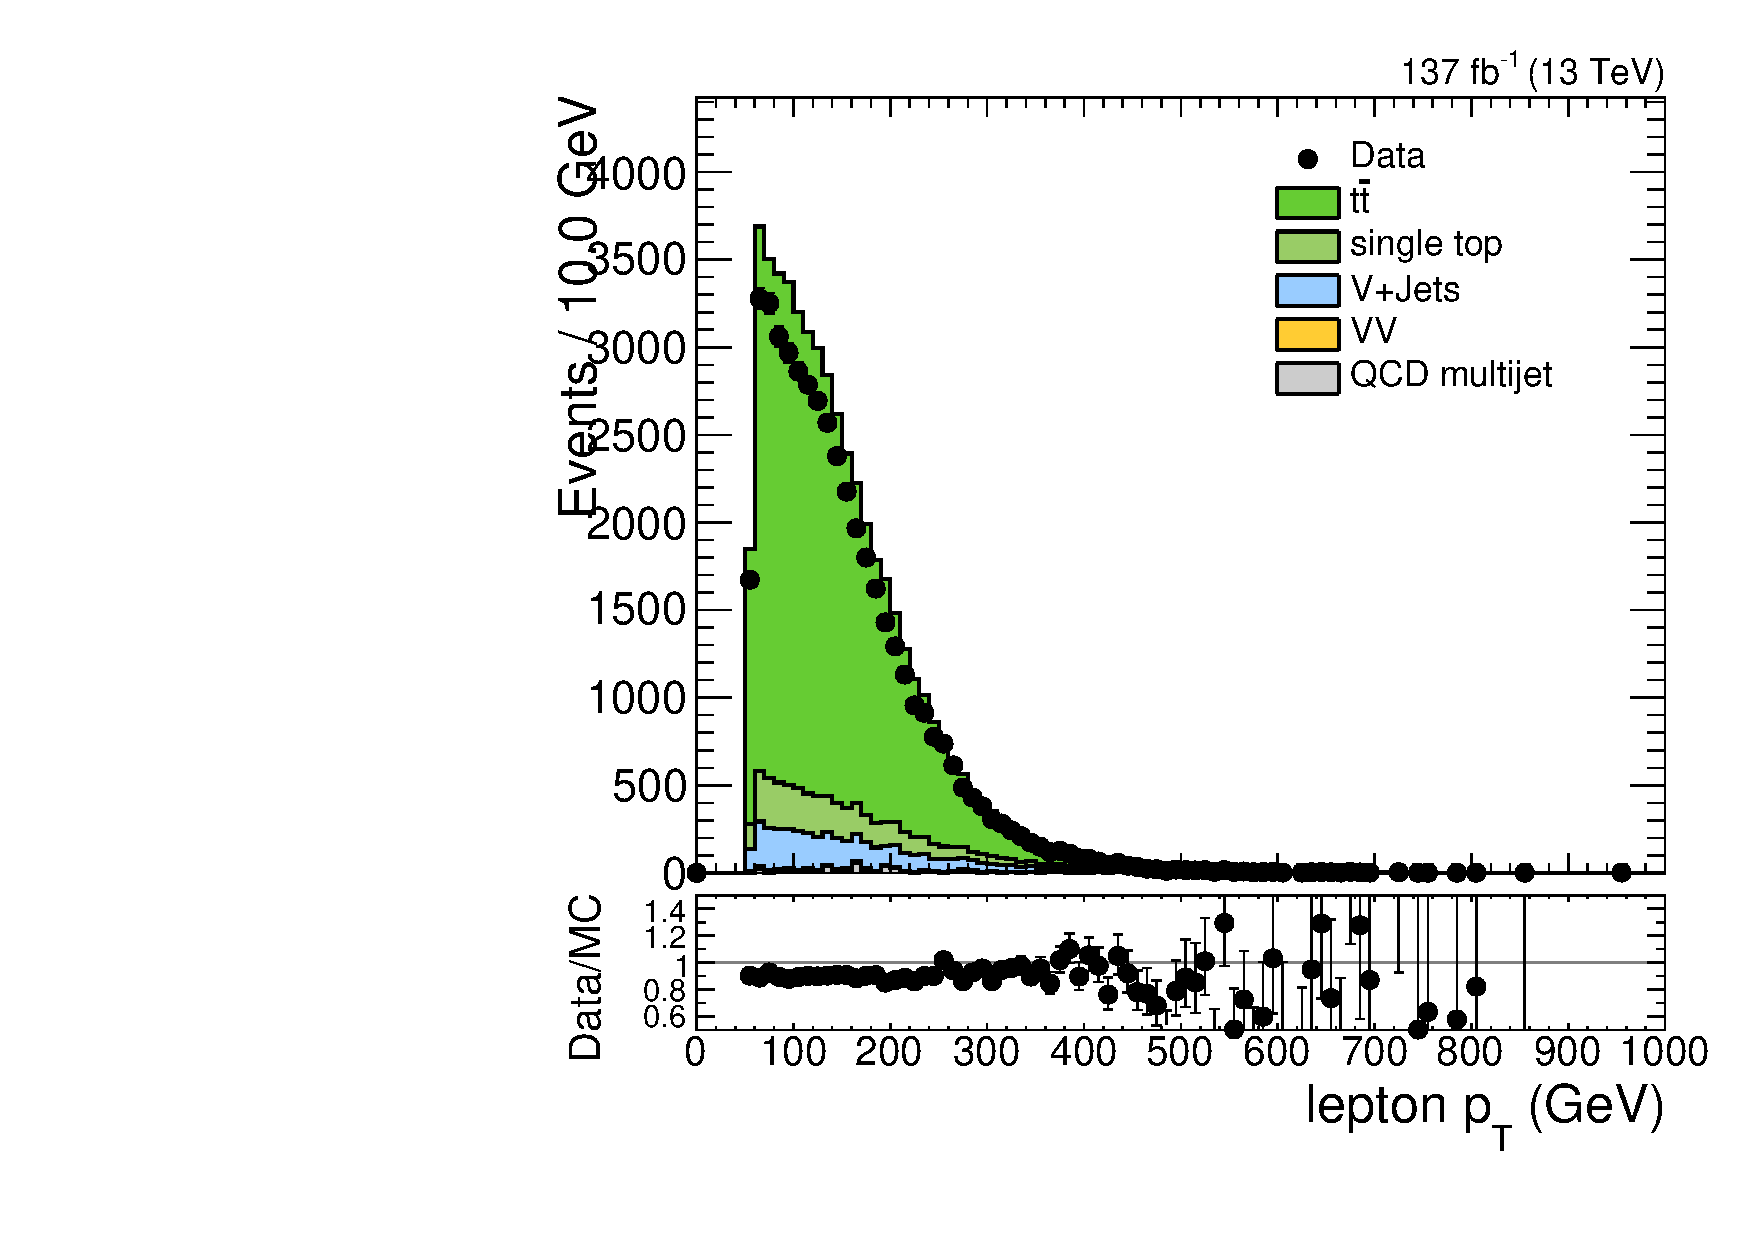
\includegraphics[width=0.3825\textwidth]{fig/controlPlots/CR_b1_e_allP_allC_allD_Run2_lnujj_l1_l_pt.pdf}\\
  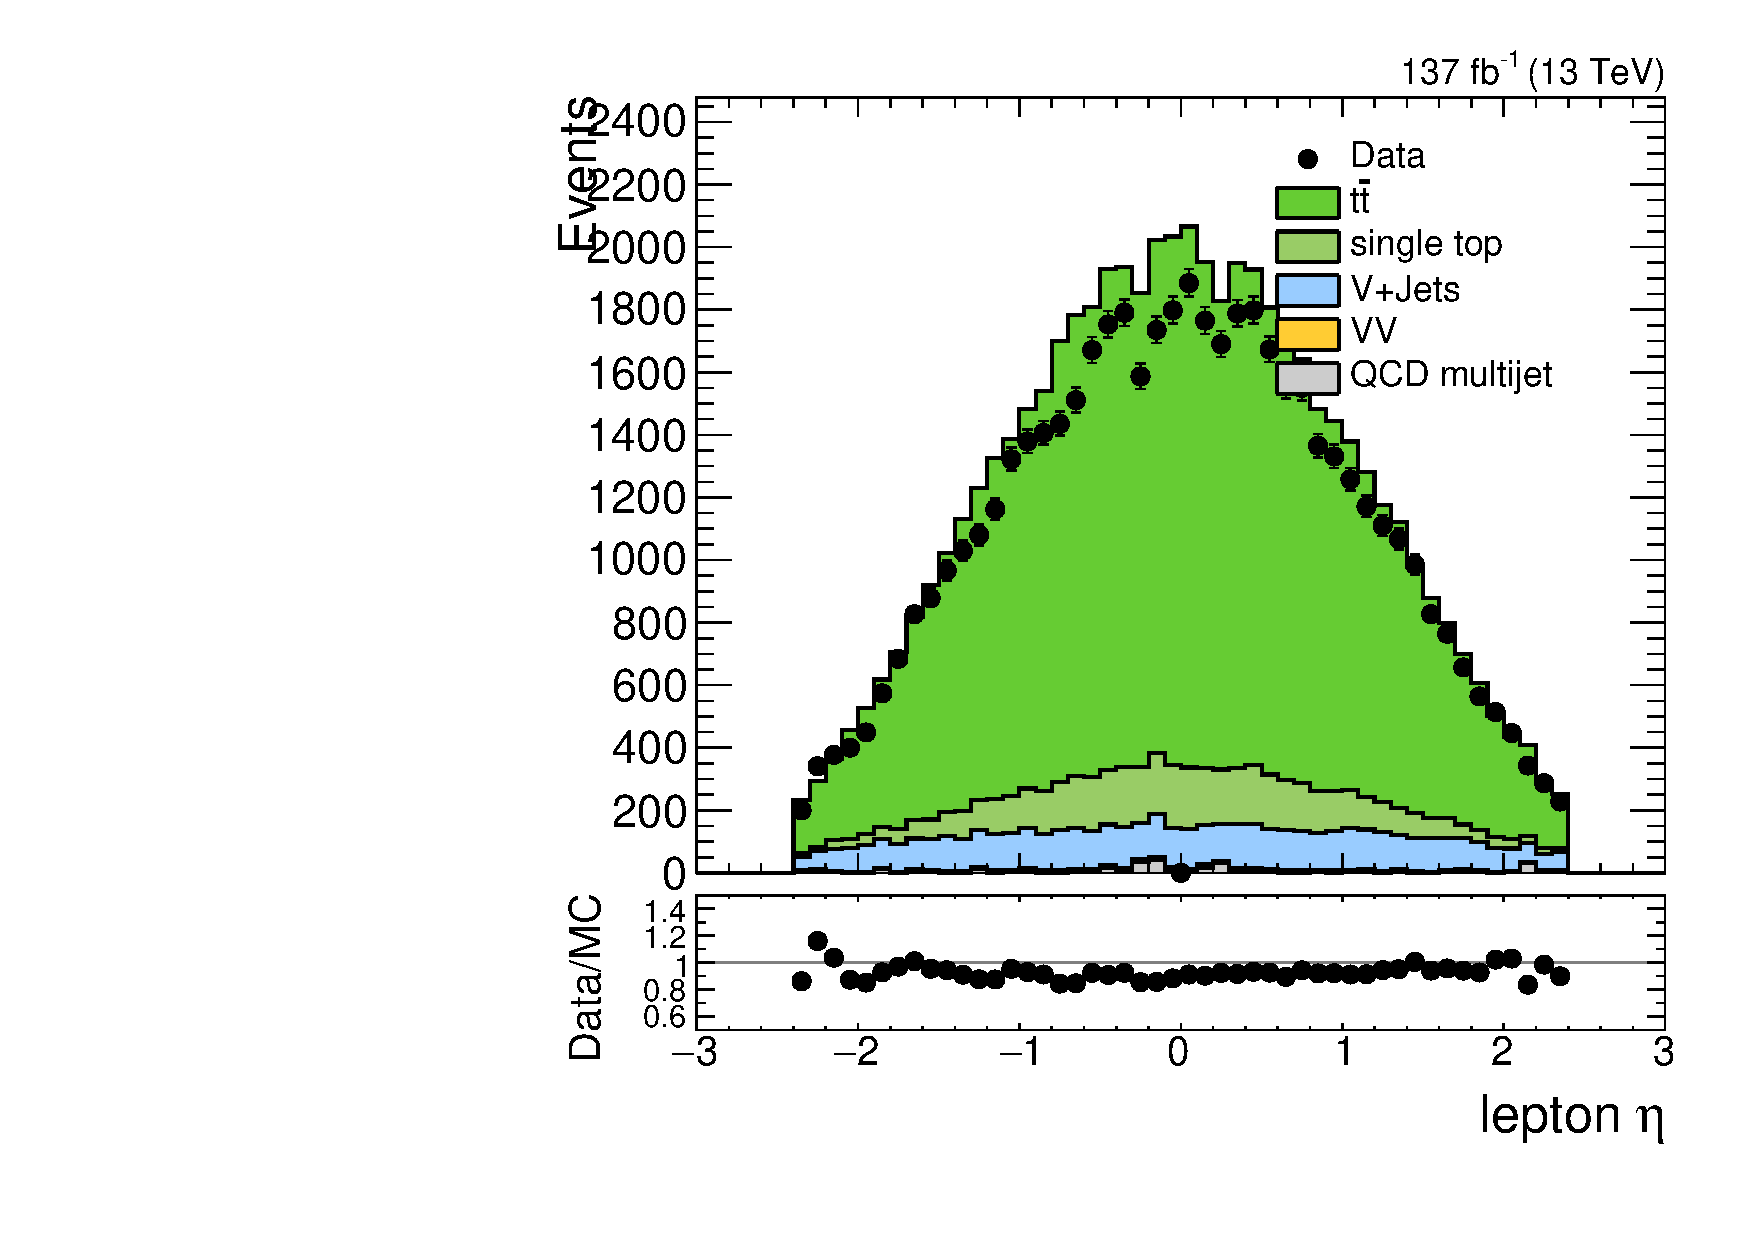
\includegraphics[width=0.3825\textwidth]{fig/controlPlots/CR_b1_mu_allP_allC_allD_Run2_lnujj_l1_l_eta.pdf}
  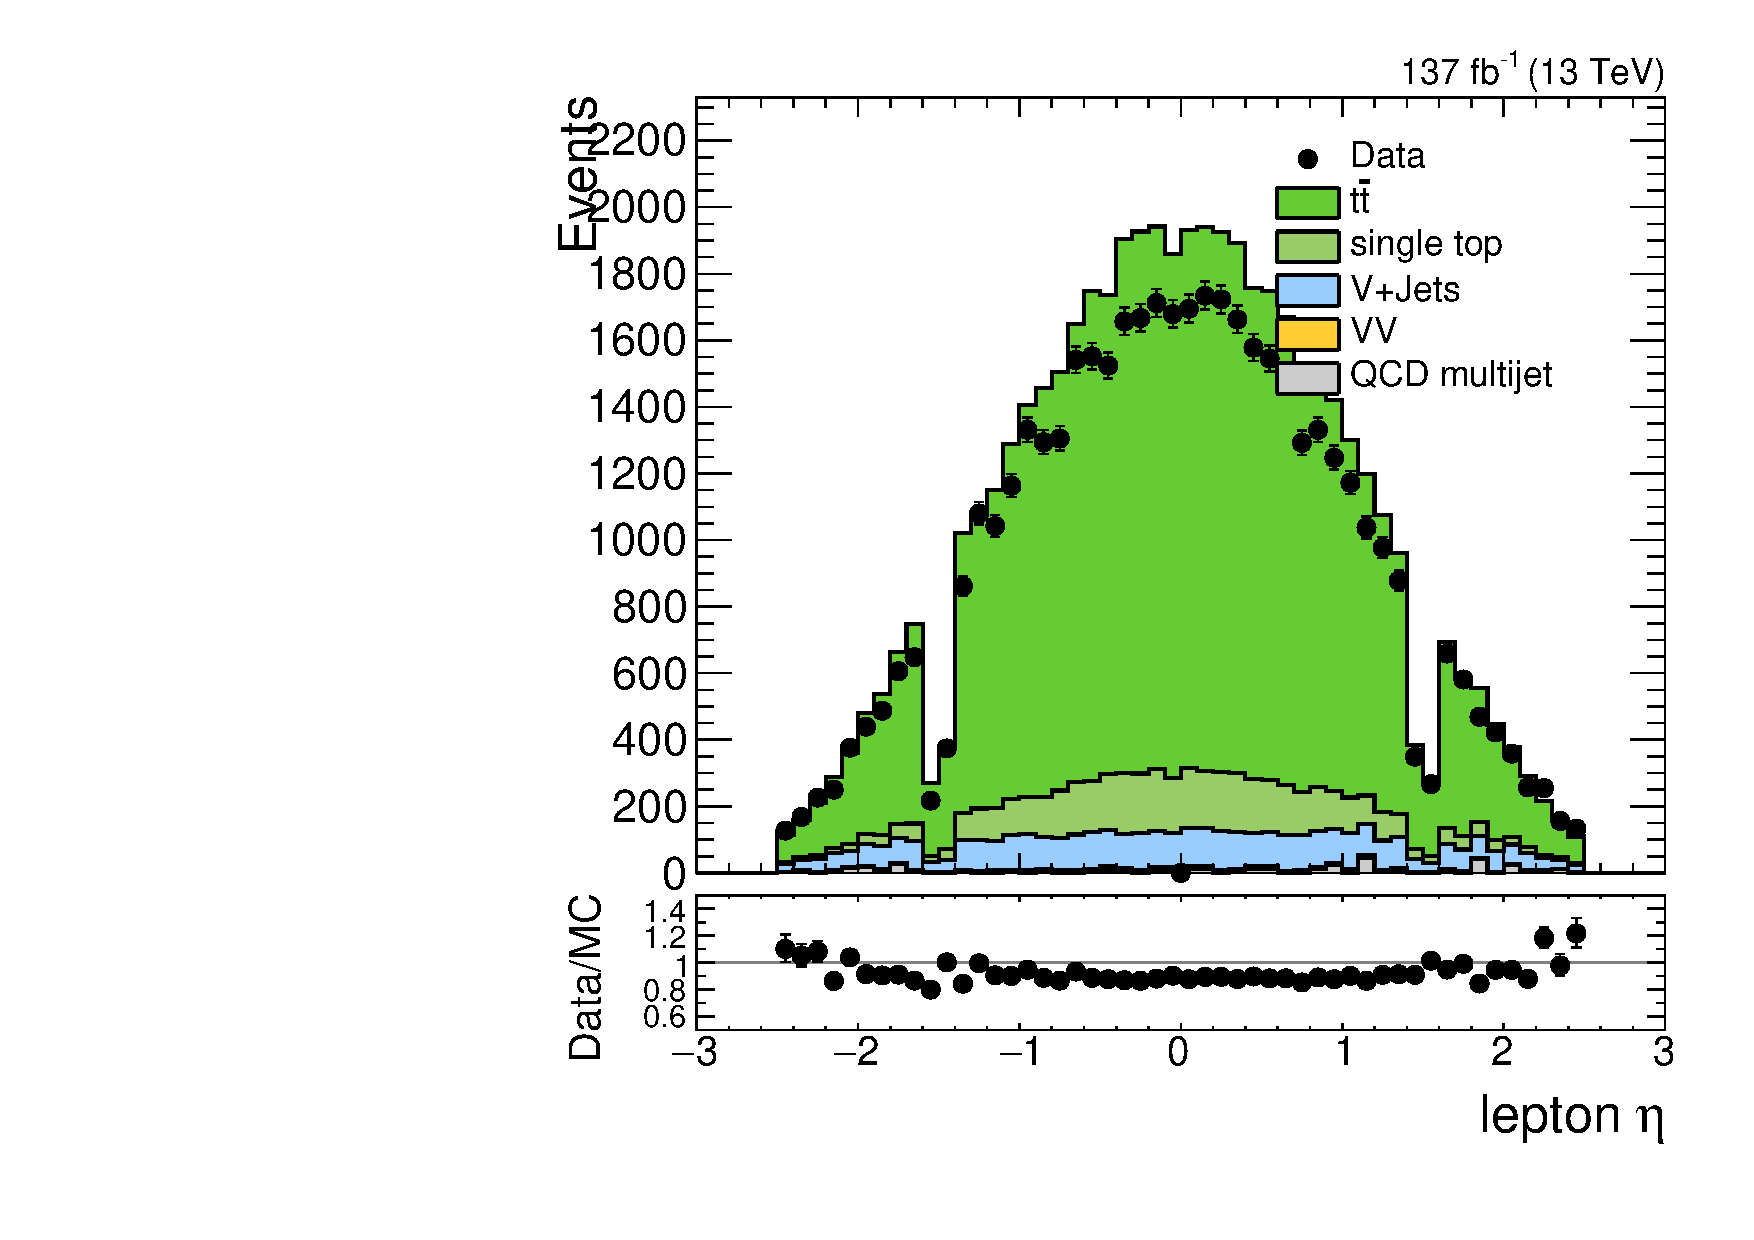
\includegraphics[width=0.3825\textwidth]{fig/controlPlots/CR_b1_e_allP_allC_allD_Run2_lnujj_l1_l_eta.pdf}\\
  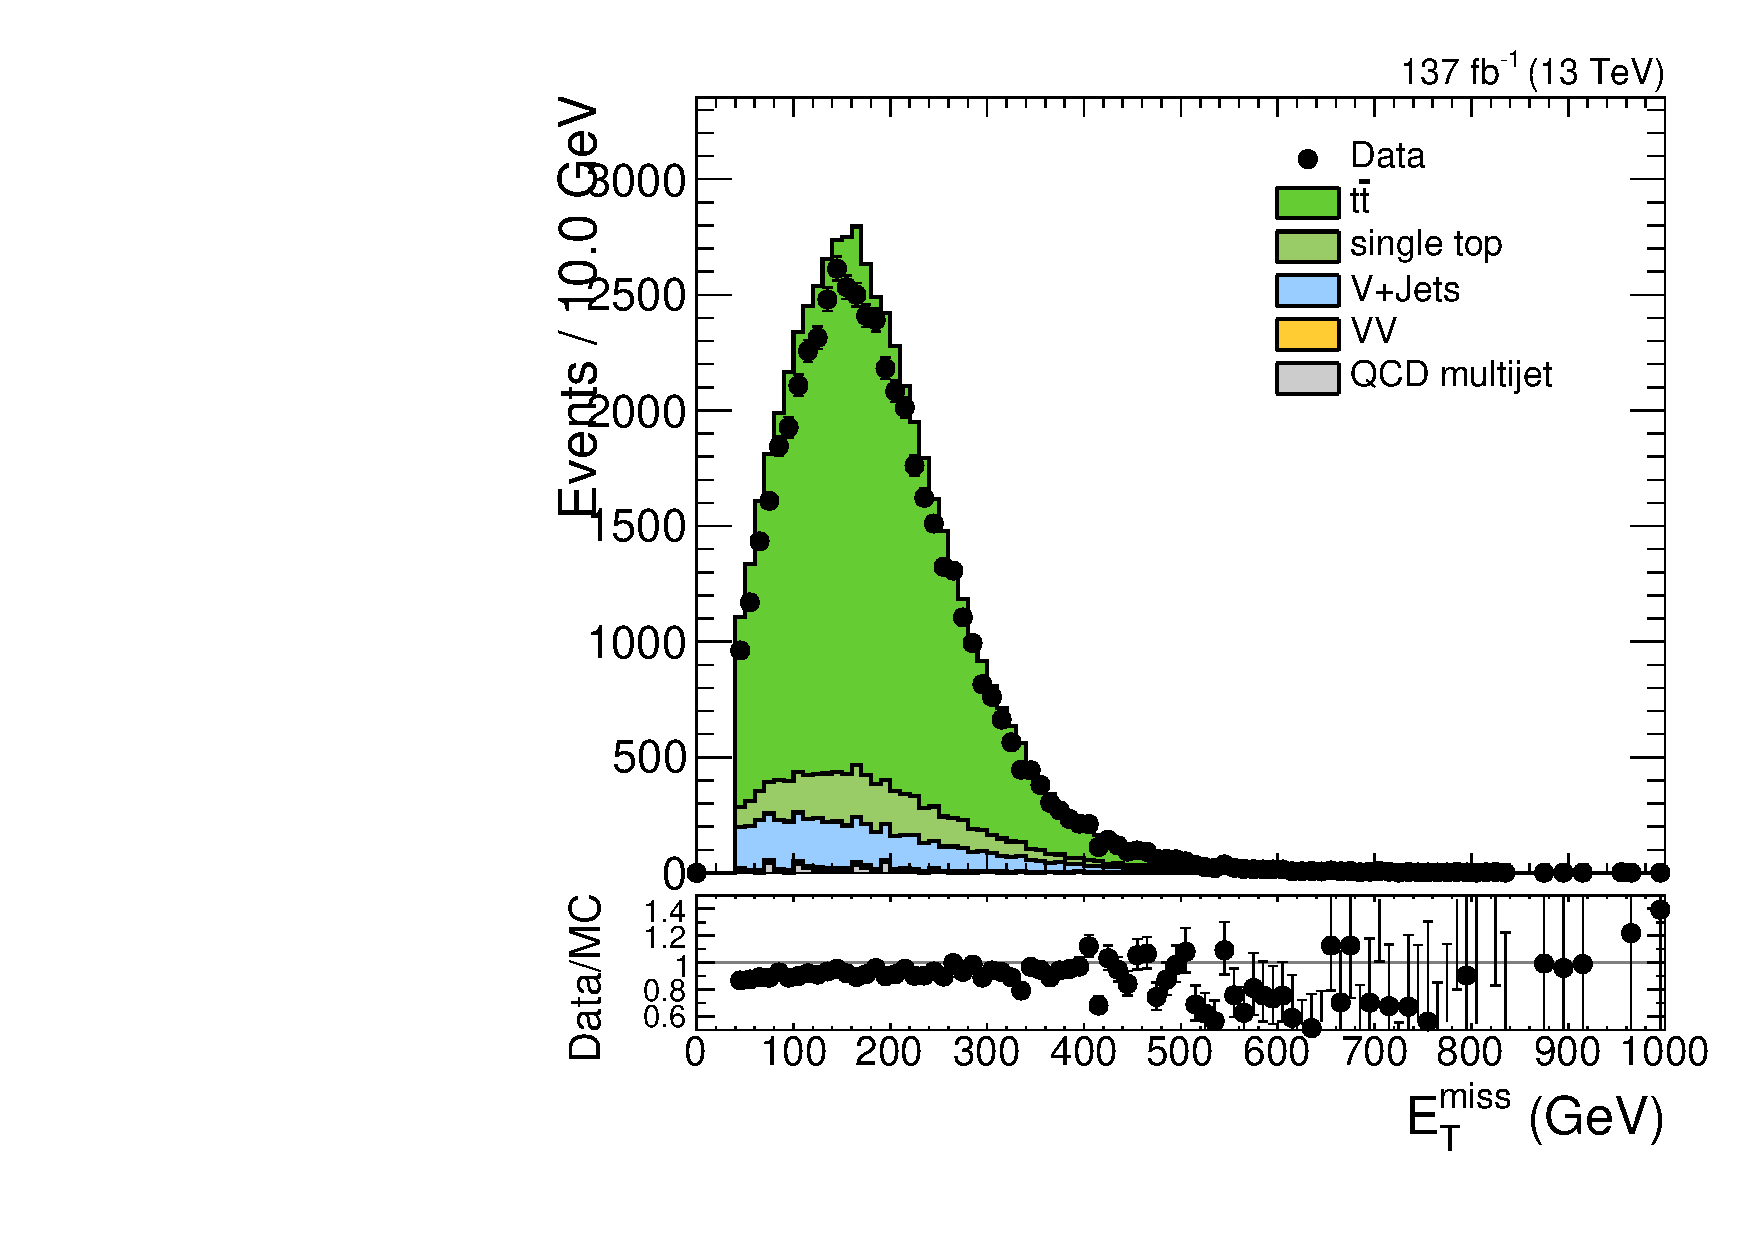
\includegraphics[width=0.3825\textwidth]{fig/controlPlots/CR_b1_mu_allP_allC_allD_Run2_met_pt.pdf}
  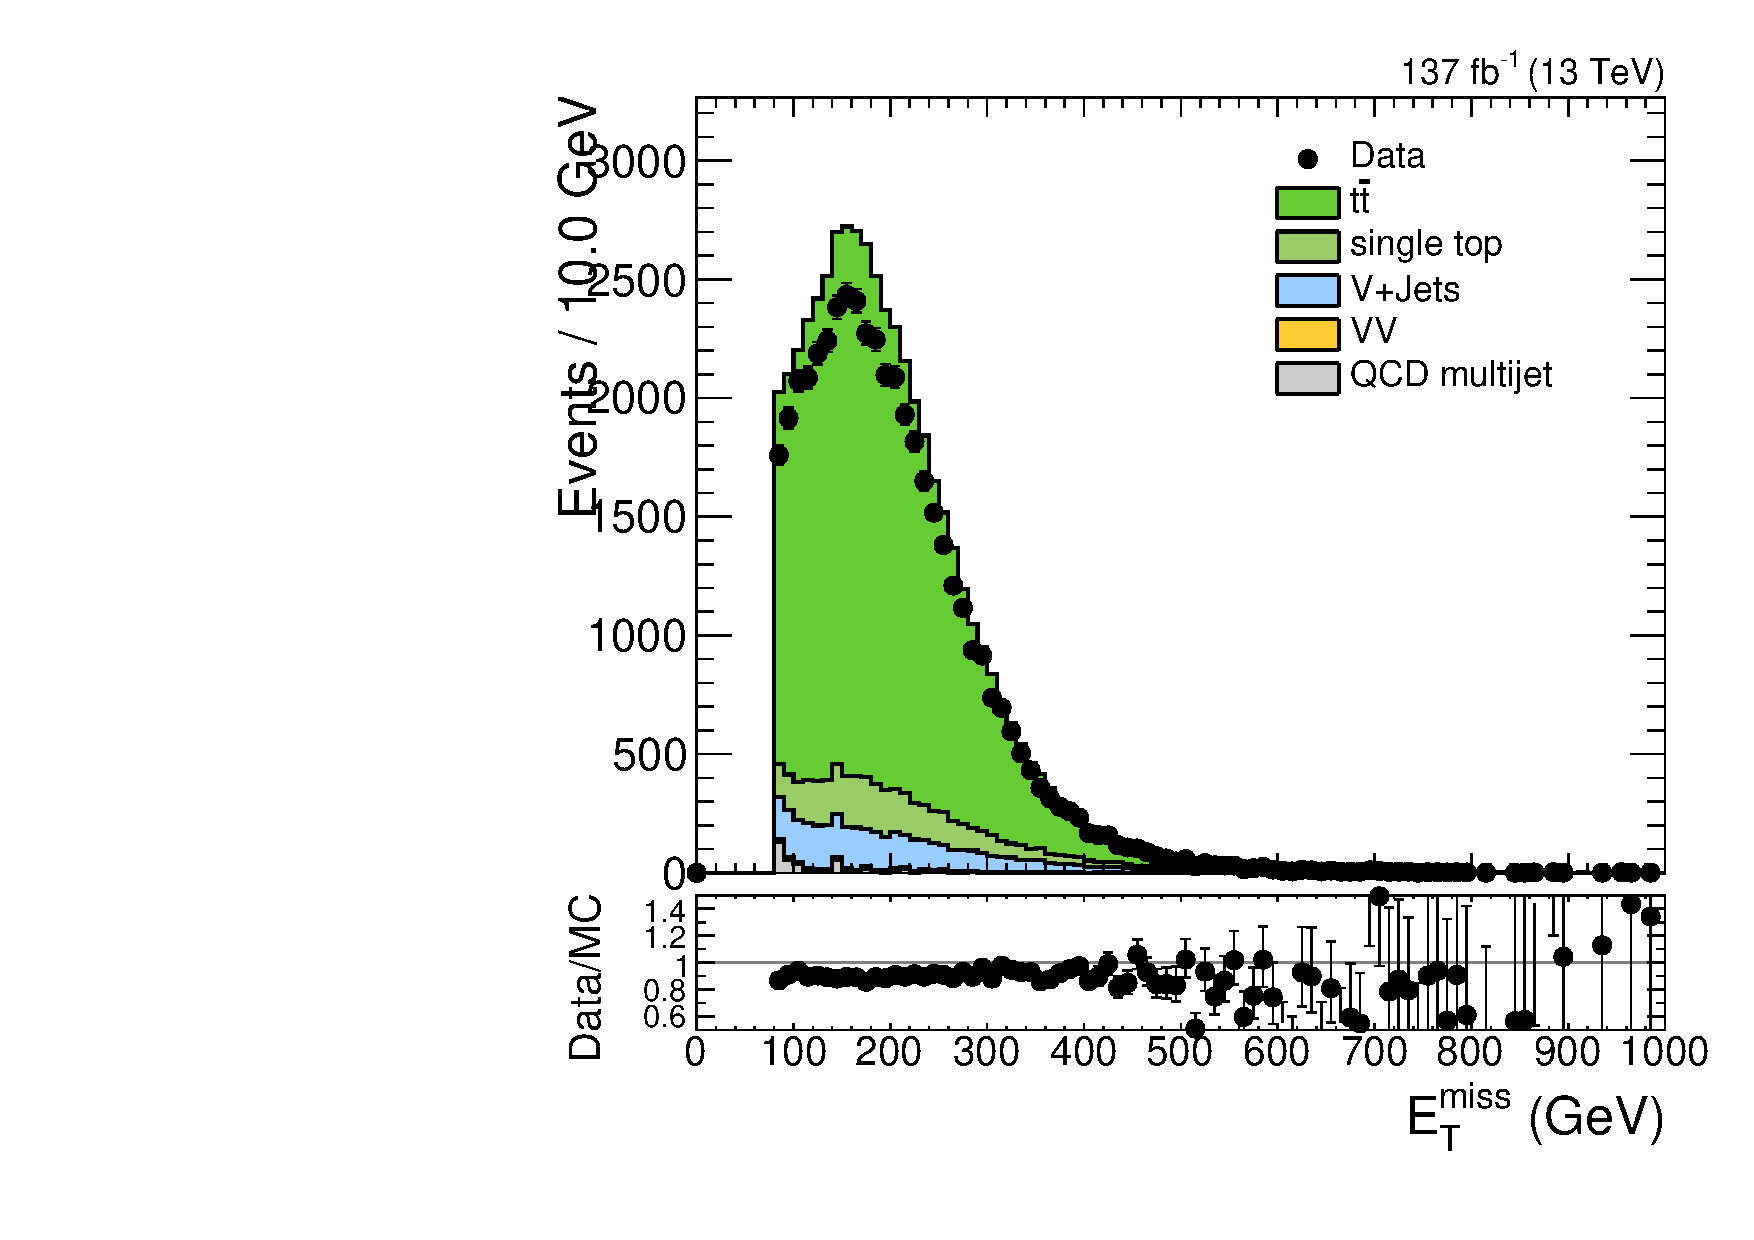
\includegraphics[width=0.3825\textwidth]{fig/controlPlots/CR_b1_e_allP_allC_allD_Run2_met_pt.pdf}\\
  \caption{
    Comparison plots between data and MC from Run 2 for different \Wlep-related observables, in the top-enriched control region.
    From top to bottom: lepton \pt, lepton $\eta$, \ptmiss.
    Left: muon channel, right: electron channel.
  }
  \label{fig:CR_controlPlotsRun2_1}
\end{figure}

\begin{figure}[htbp]
  \centering
  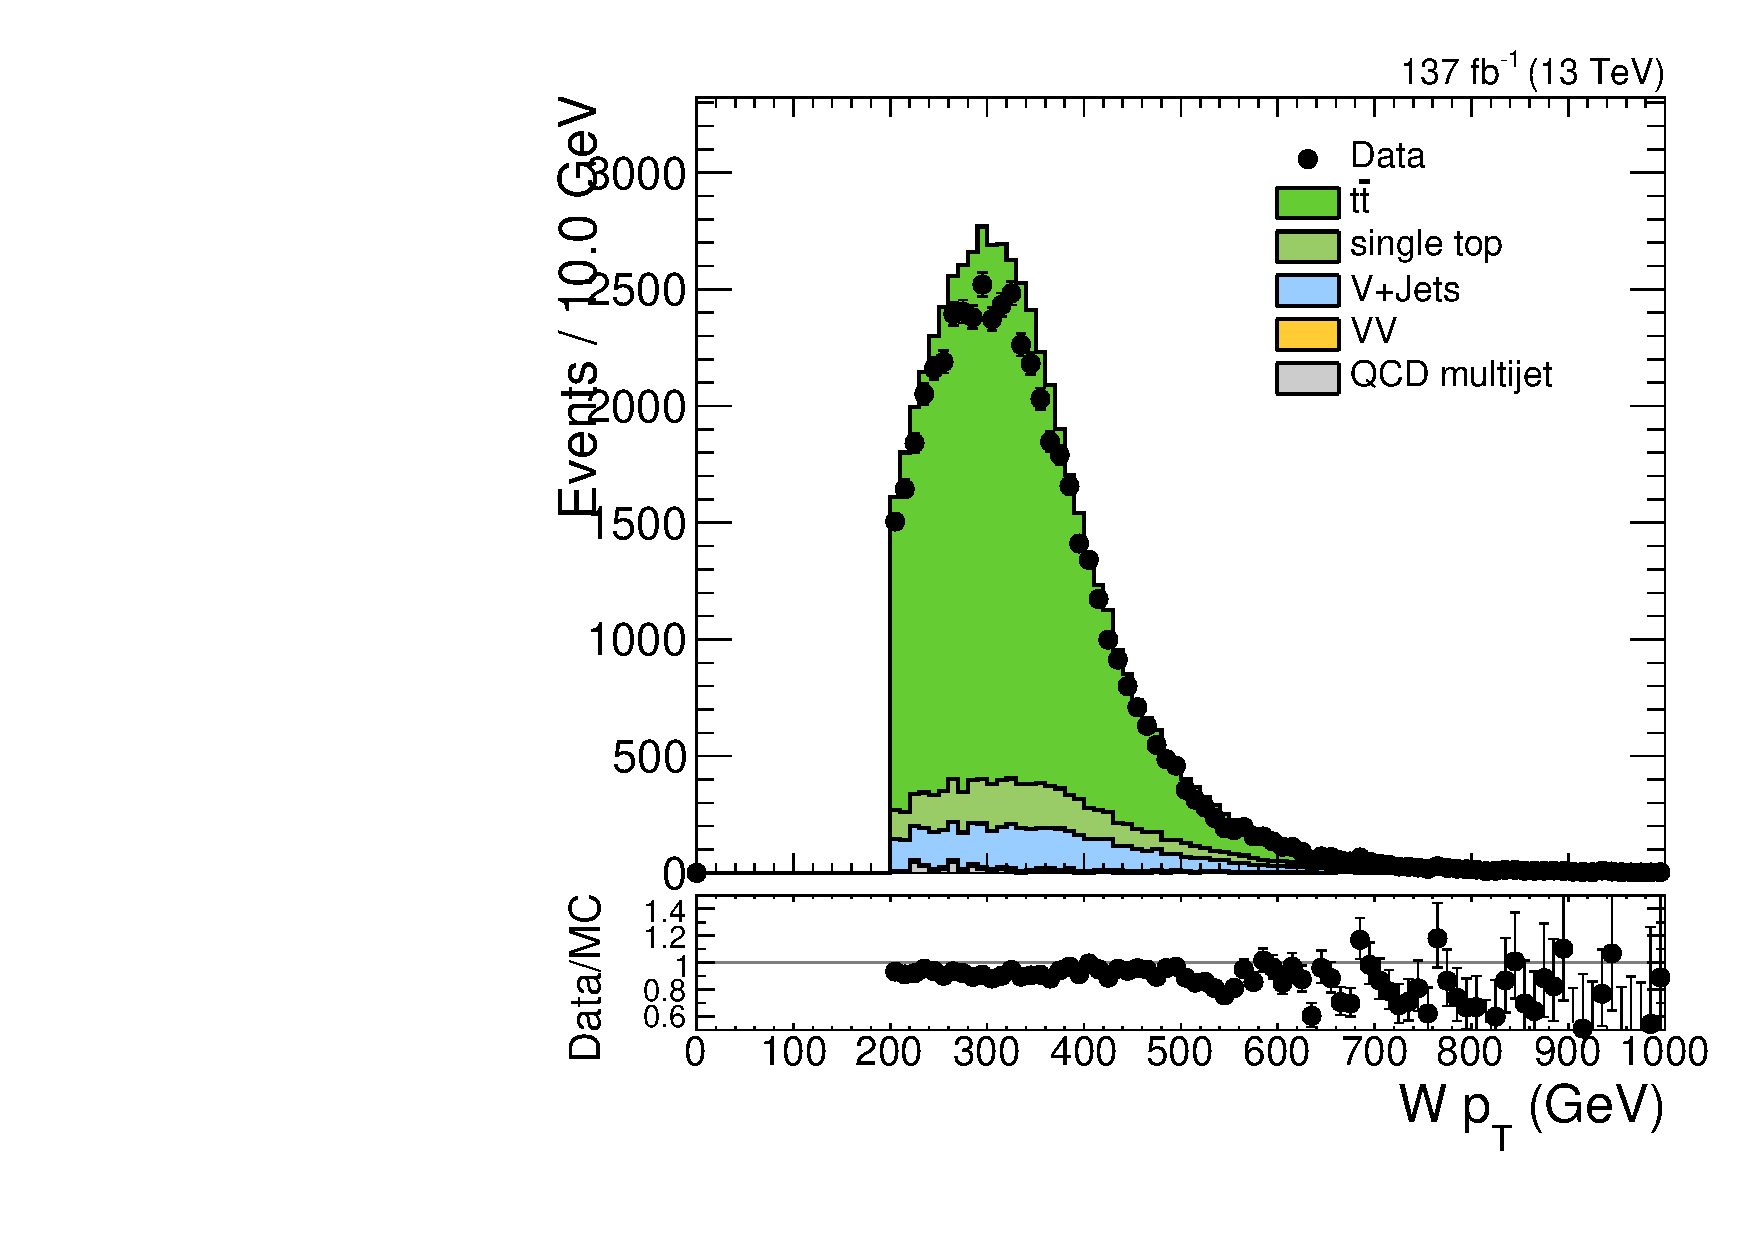
\includegraphics[width=0.3825\textwidth]{fig/controlPlots/CR_b1_mu_allP_allC_allD_Run2_lnujj_l1_pt.pdf}
  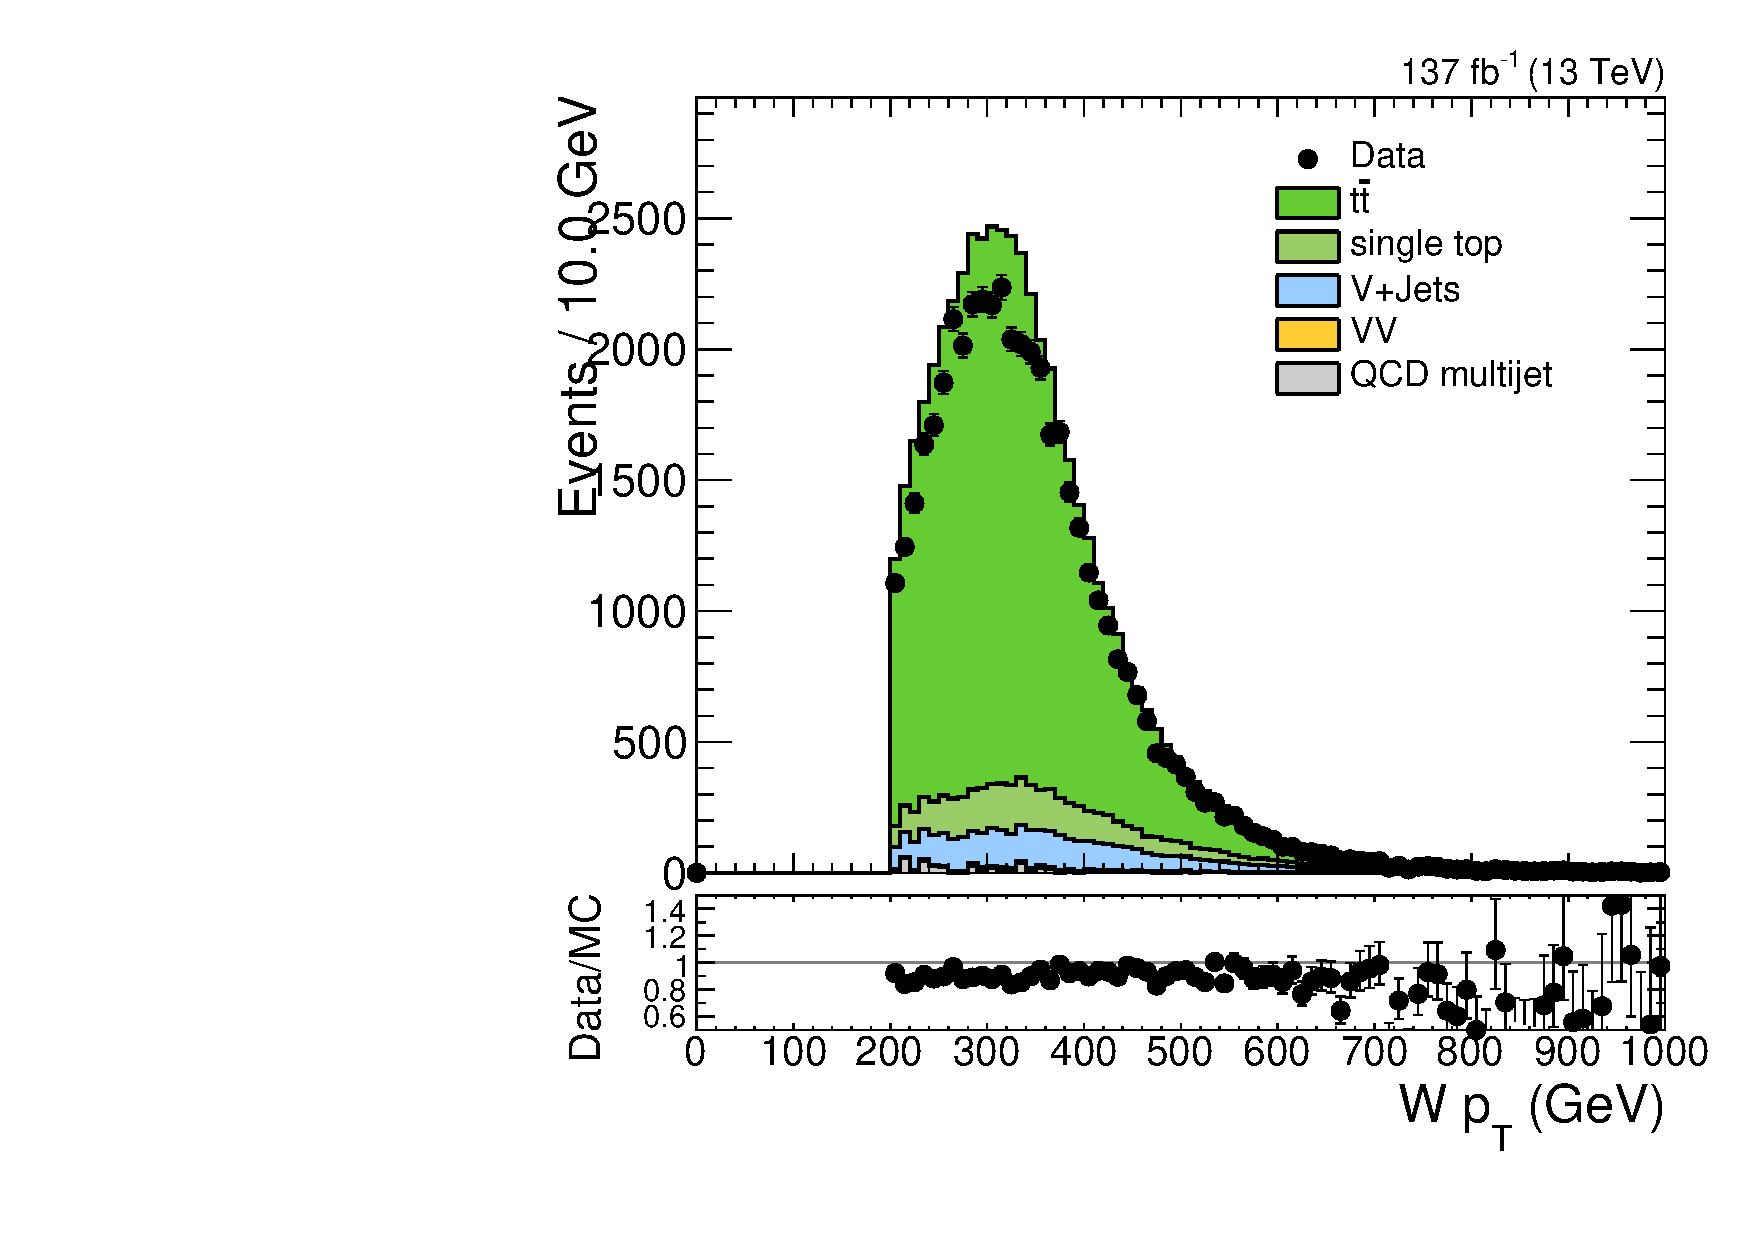
\includegraphics[width=0.3825\textwidth]{fig/controlPlots/CR_b1_e_allP_allC_allD_Run2_lnujj_l1_pt.pdf}\\
  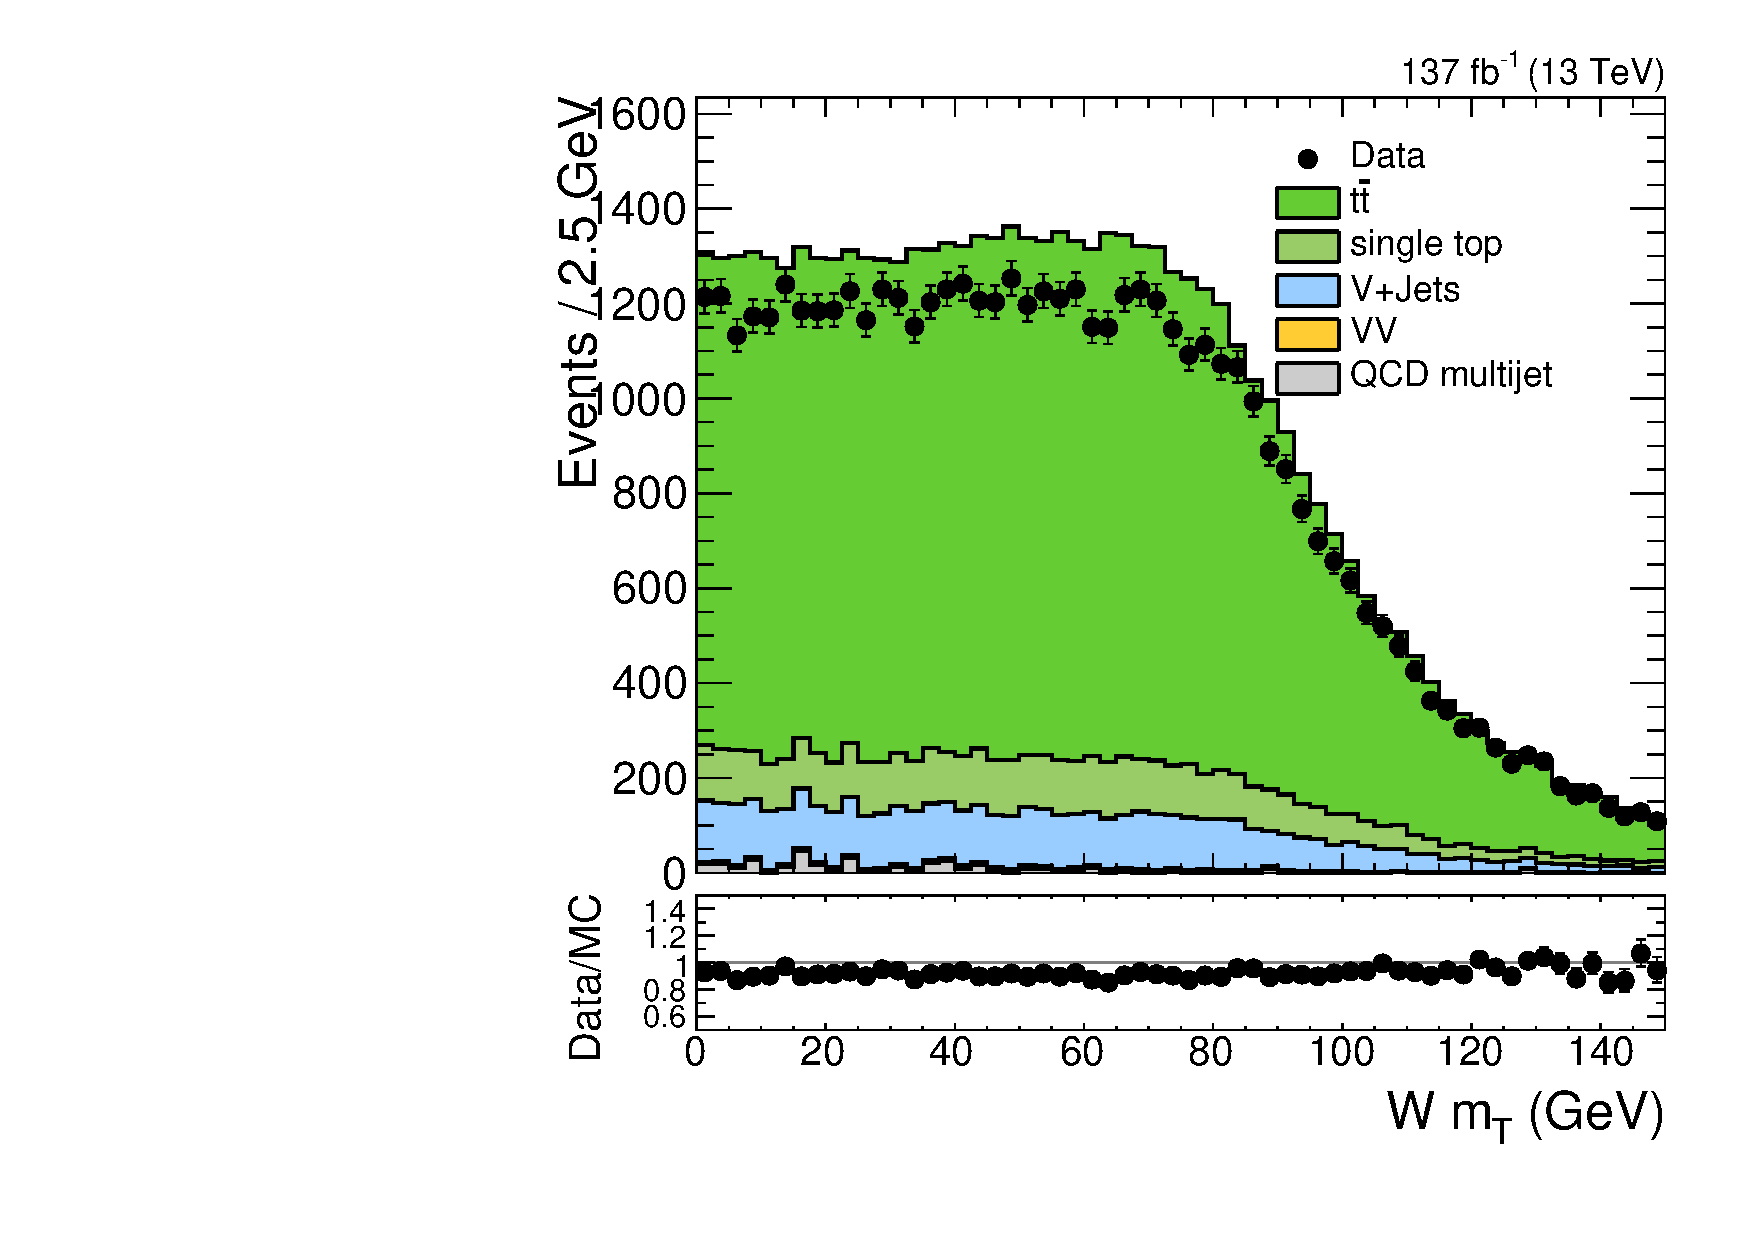
\includegraphics[width=0.3825\textwidth]{fig/controlPlots/CR_b1_mu_allP_allC_allD_Run2_lnujj_l1_mt.pdf}
  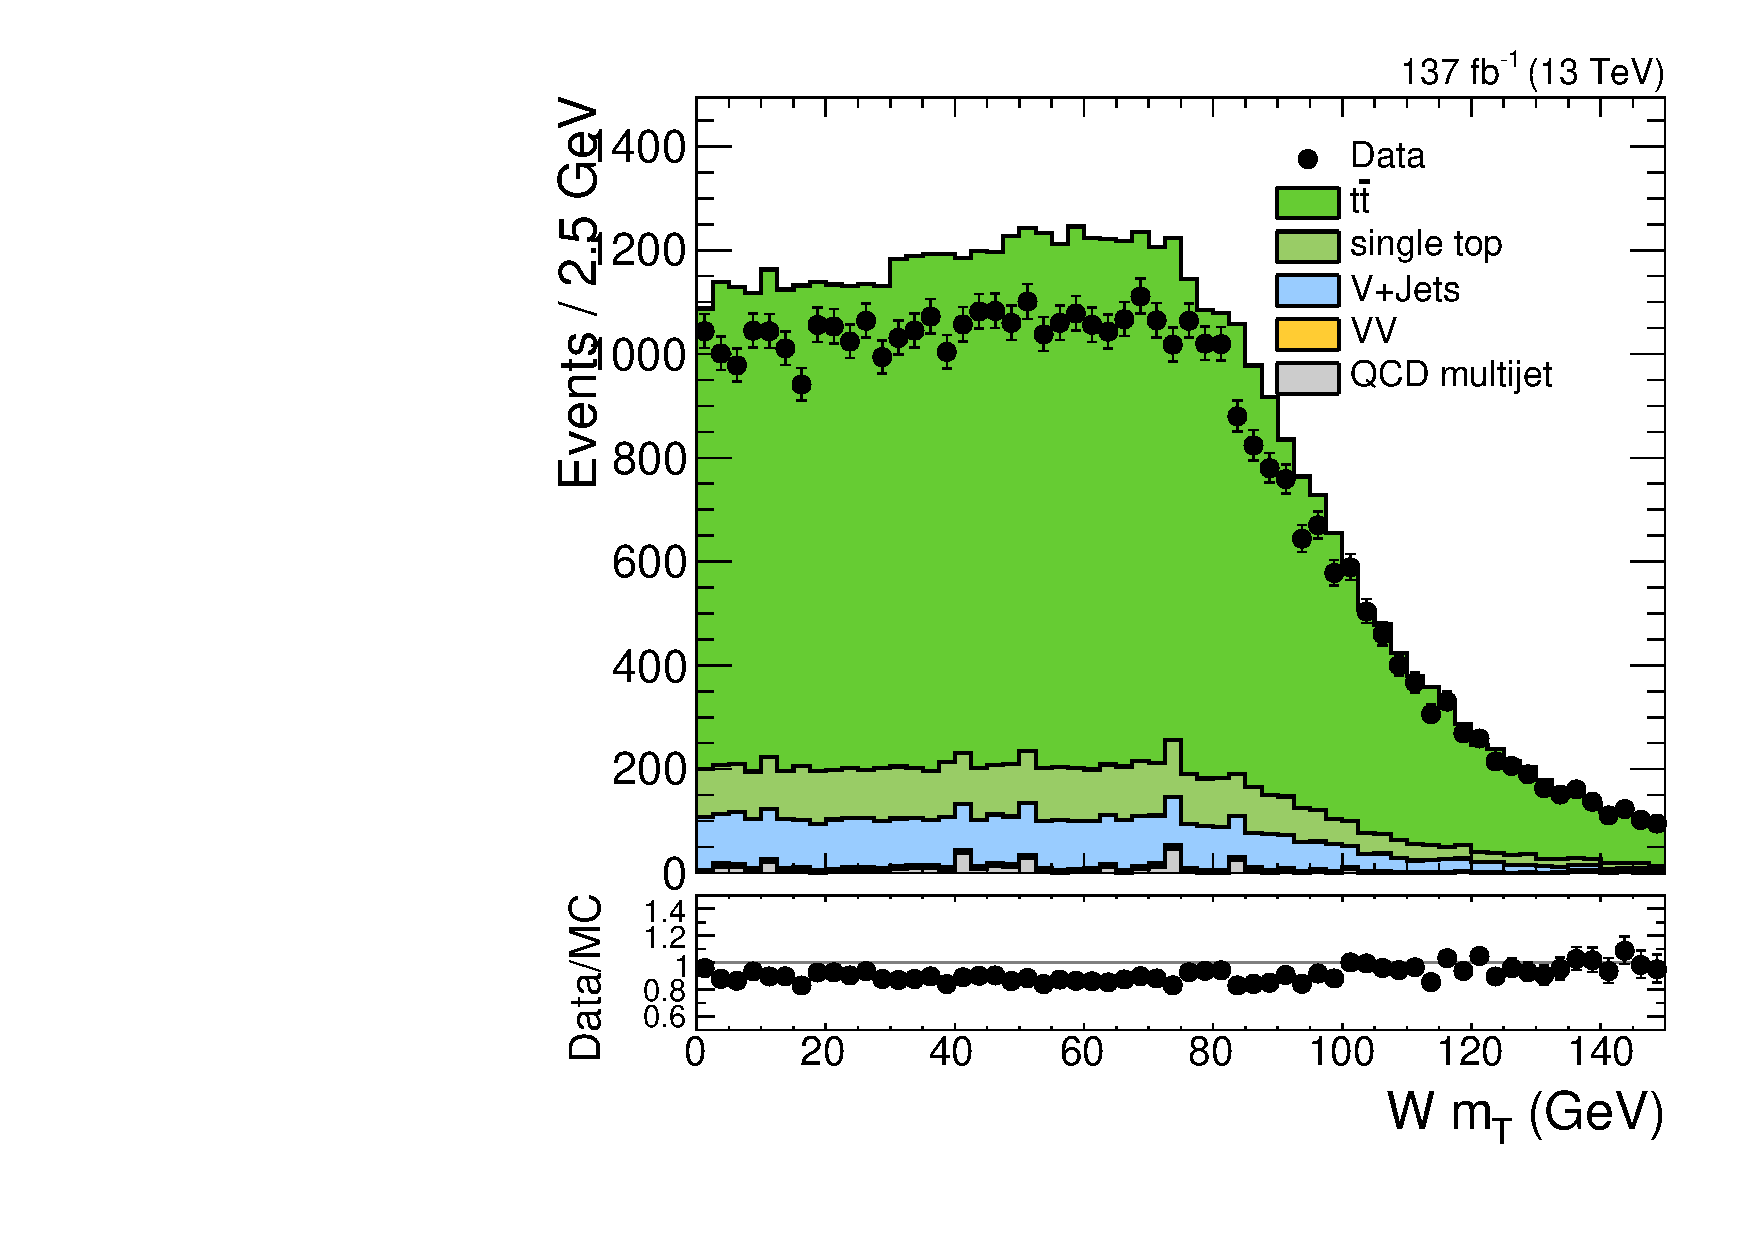
\includegraphics[width=0.3825\textwidth]{fig/controlPlots/CR_b1_e_allP_allC_allD_Run2_lnujj_l1_mt.pdf}\\
  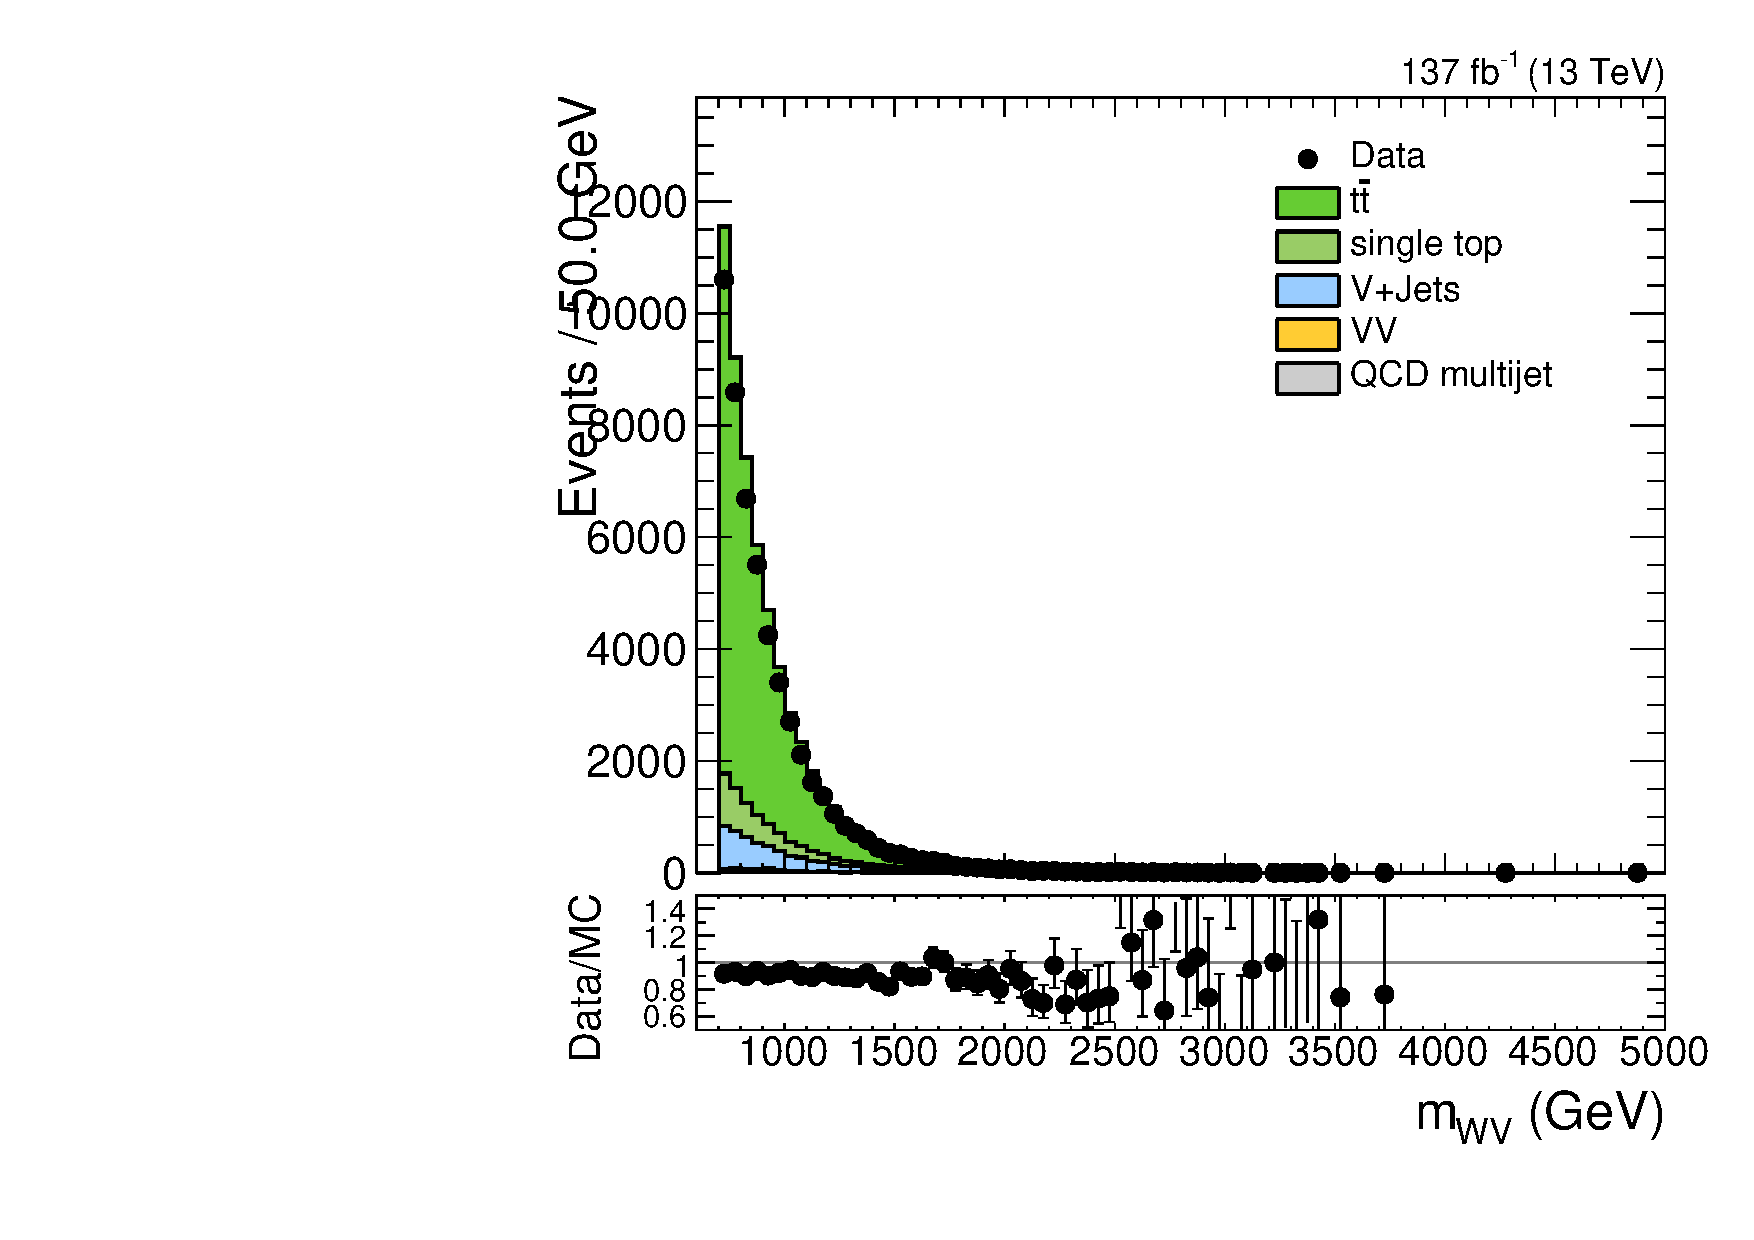
\includegraphics[width=0.3825\textwidth]{fig/controlPlots/CR_b1_mu_allP_allC_allD_Run2_mWV.pdf}
  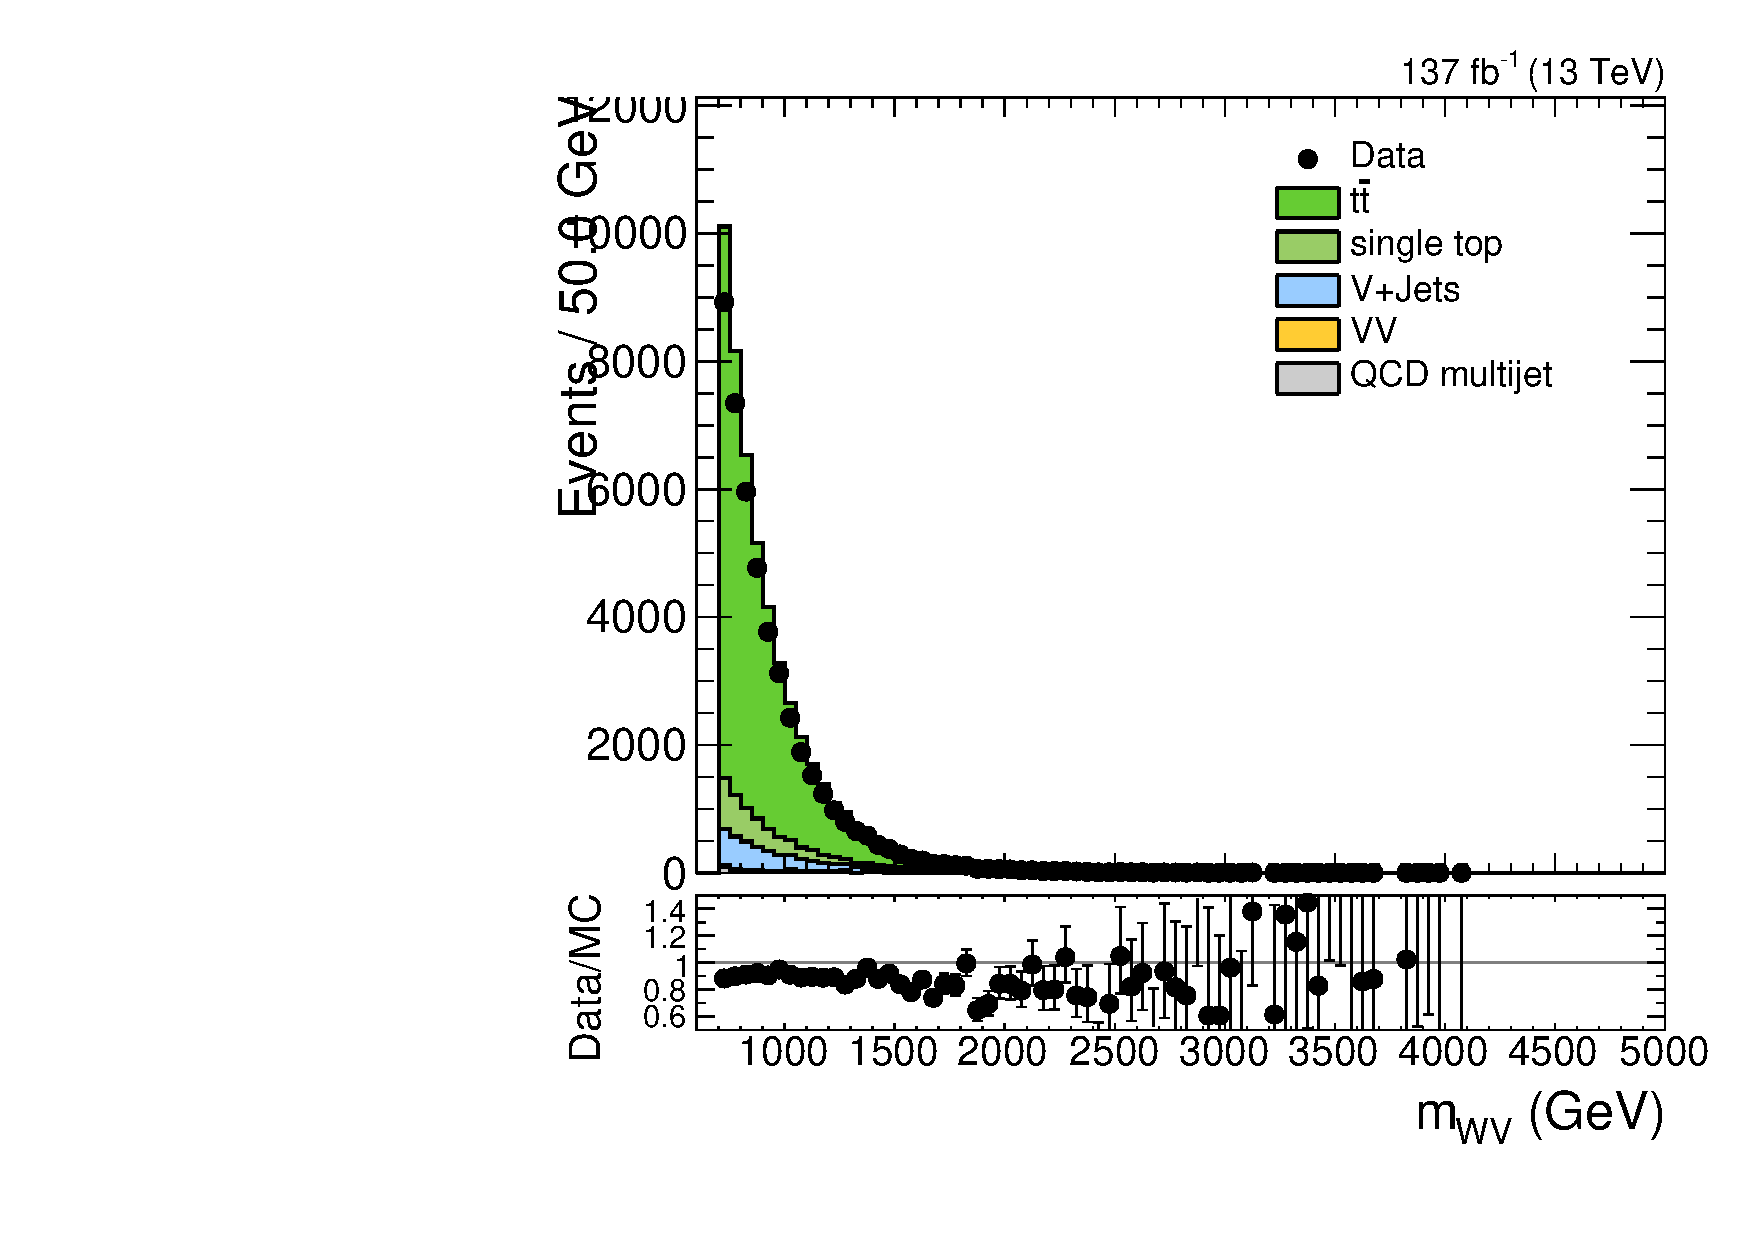
\includegraphics[width=0.3825\textwidth]{fig/controlPlots/CR_b1_e_allP_allC_allD_Run2_mWV.pdf}\\
  \caption{
    Comparison plots between data and MC from Run 2 for different \Wlep-related observables, in the top-enriched control region.
    From top to bottom: \pt of the leptonic $W$, transverse mass of the leptonic $W$, diboson invariant mass.
    Left: muon channel, right: electron channel.
  }
  \label{fig:CR_controlPlotsRun2_2}
\end{figure}

\begin{figure}[htbp]
  \centering
  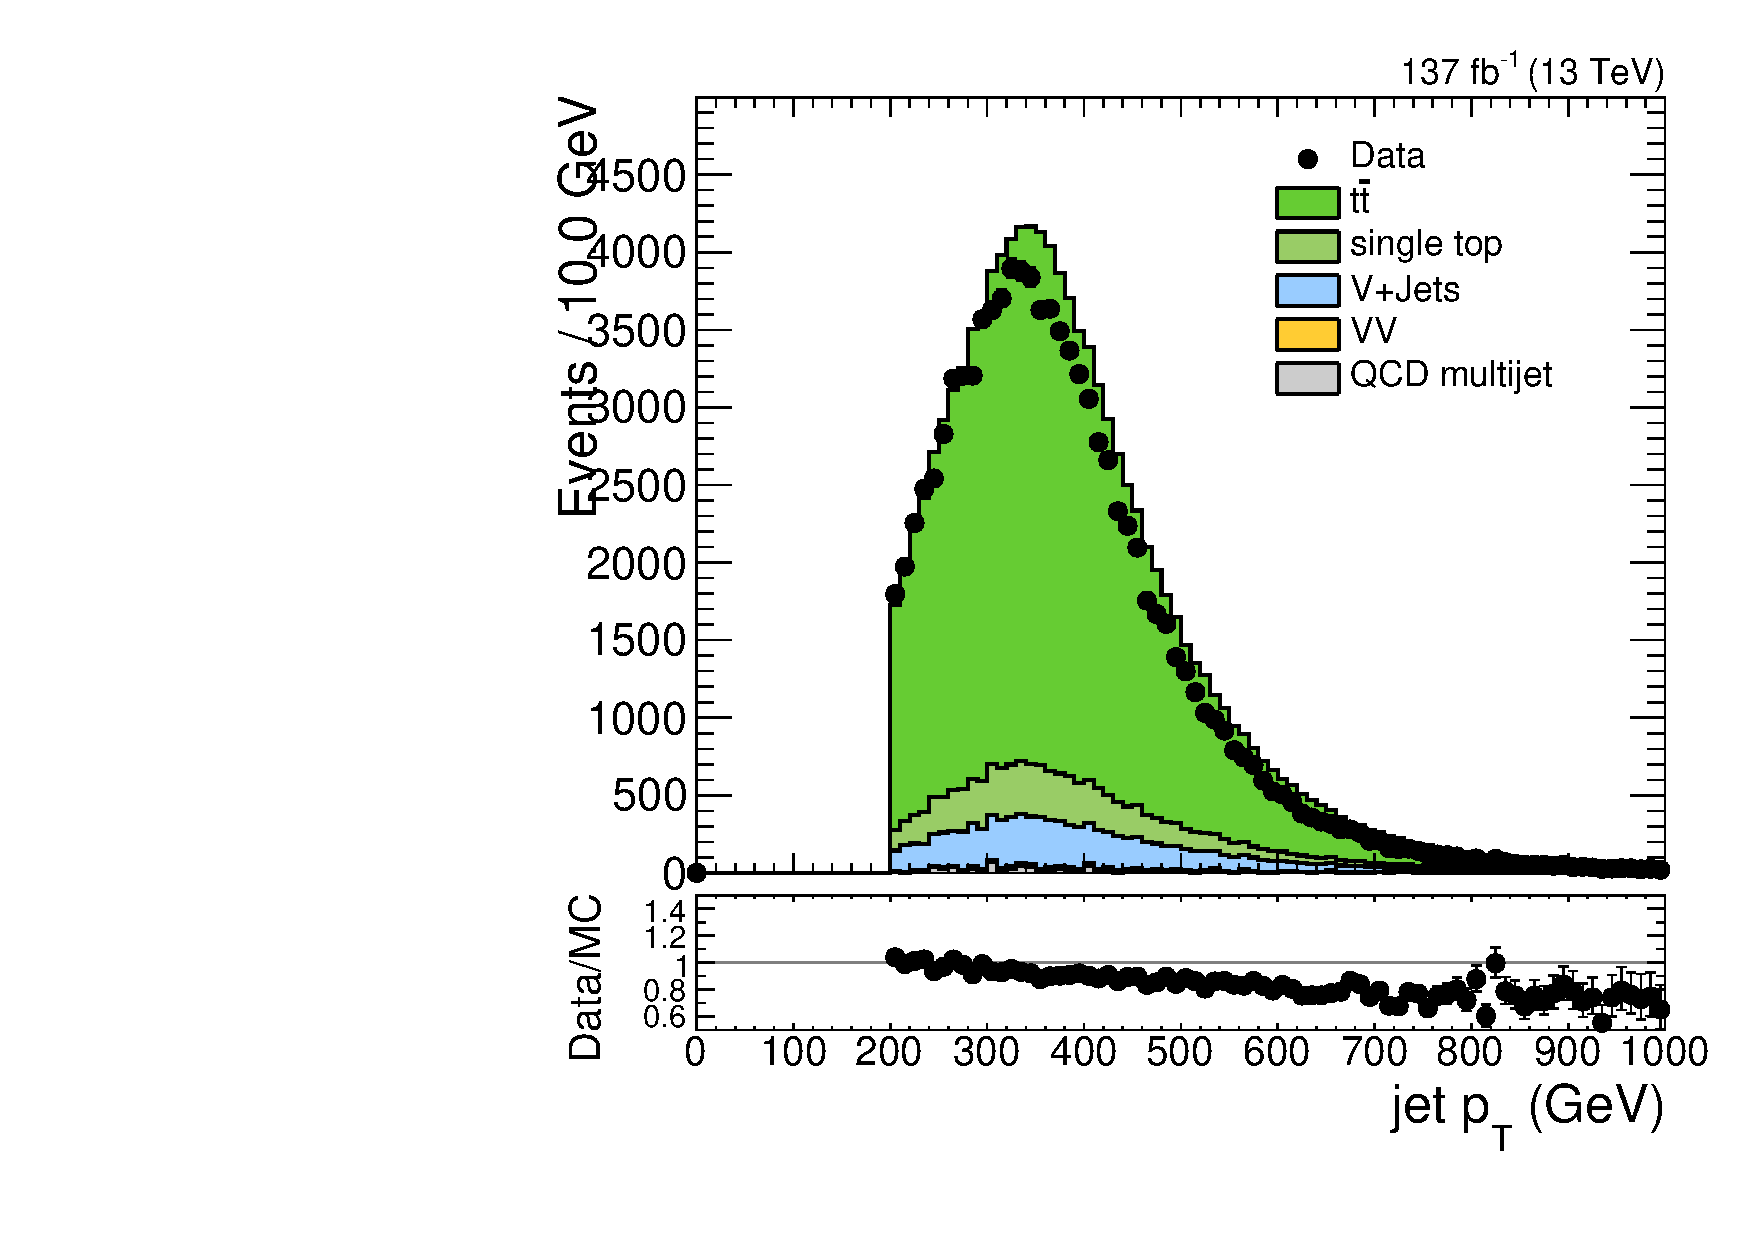
\includegraphics[width=0.3825\textwidth]{fig/controlPlots/CR_b1_allL_allP_allC_allD_Run2_lnujj_l2_pt.pdf}
  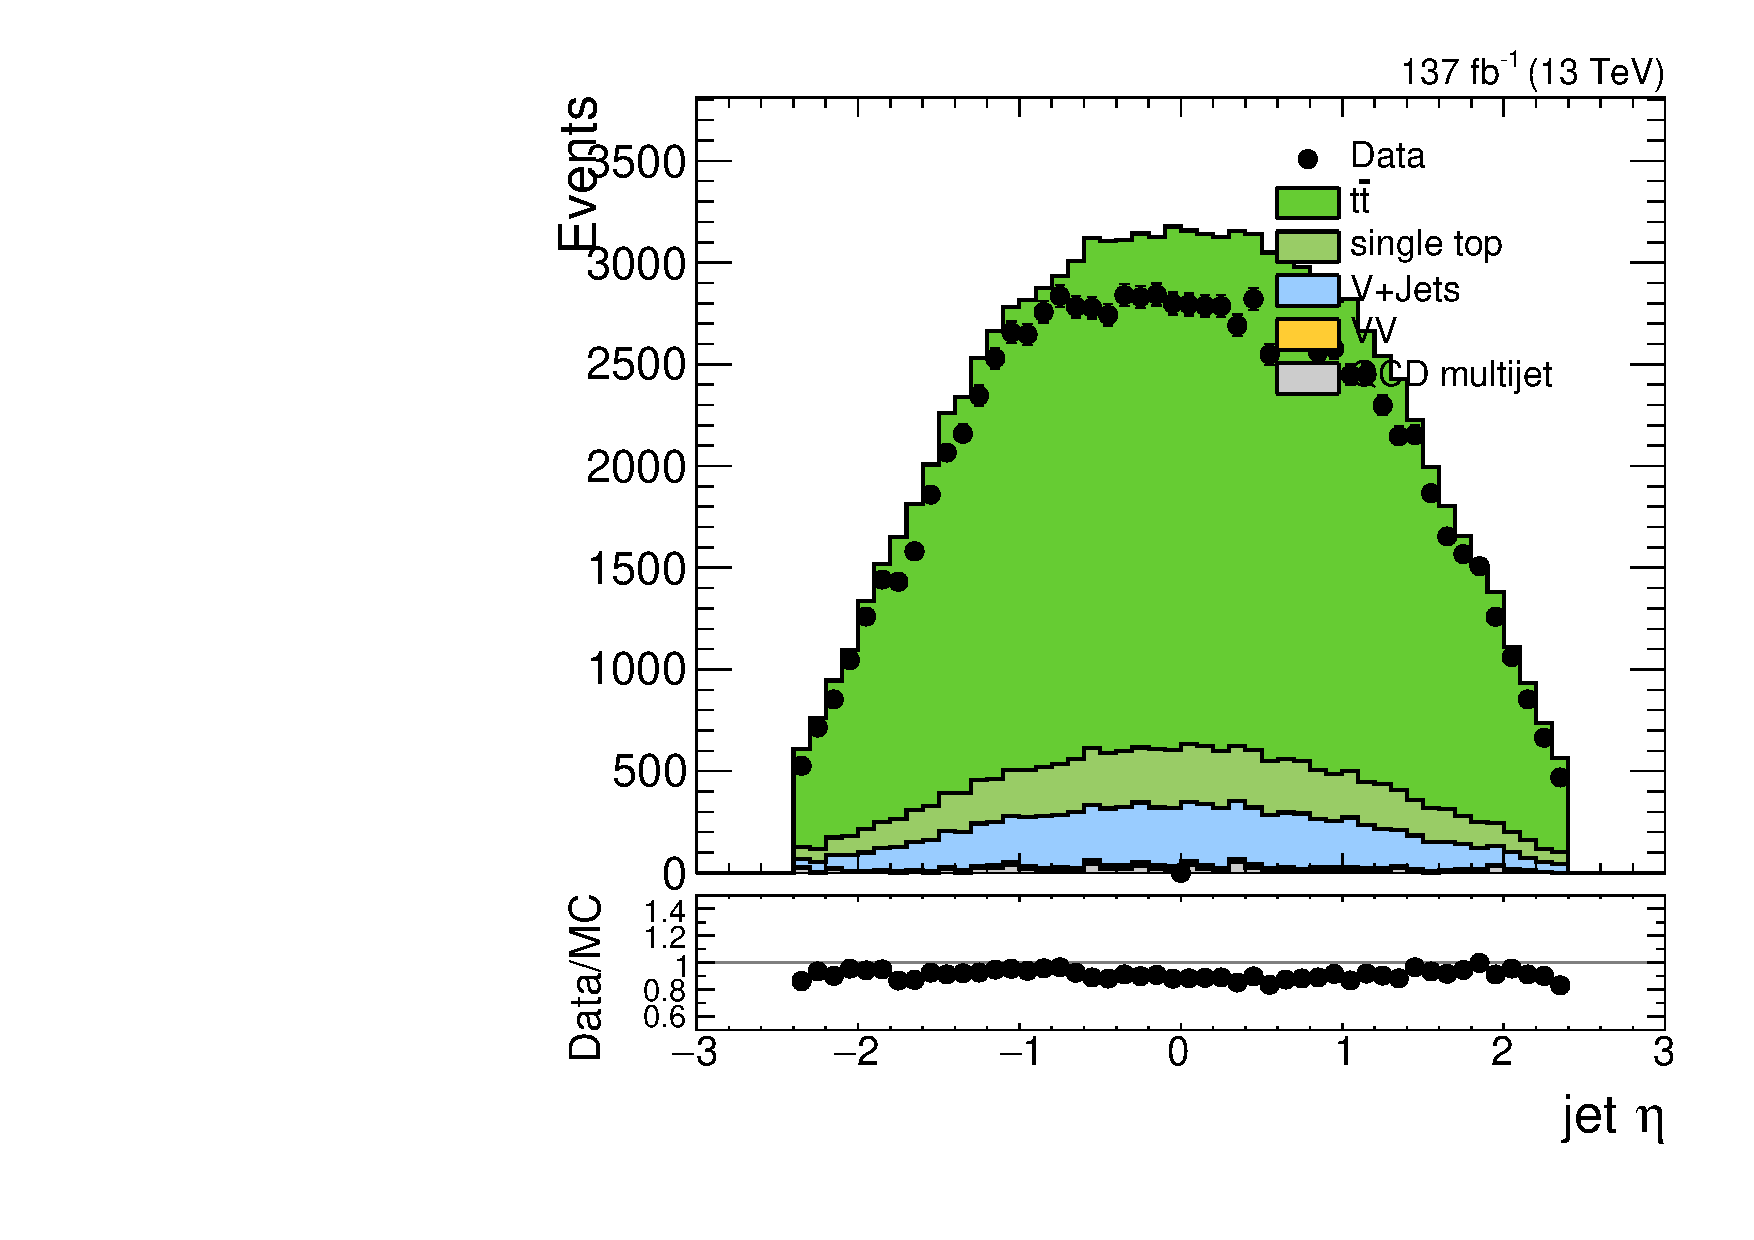
\includegraphics[width=0.3825\textwidth]{fig/controlPlots/CR_b1_allL_allP_allC_allD_Run2_lnujj_l2_eta.pdf}\\
  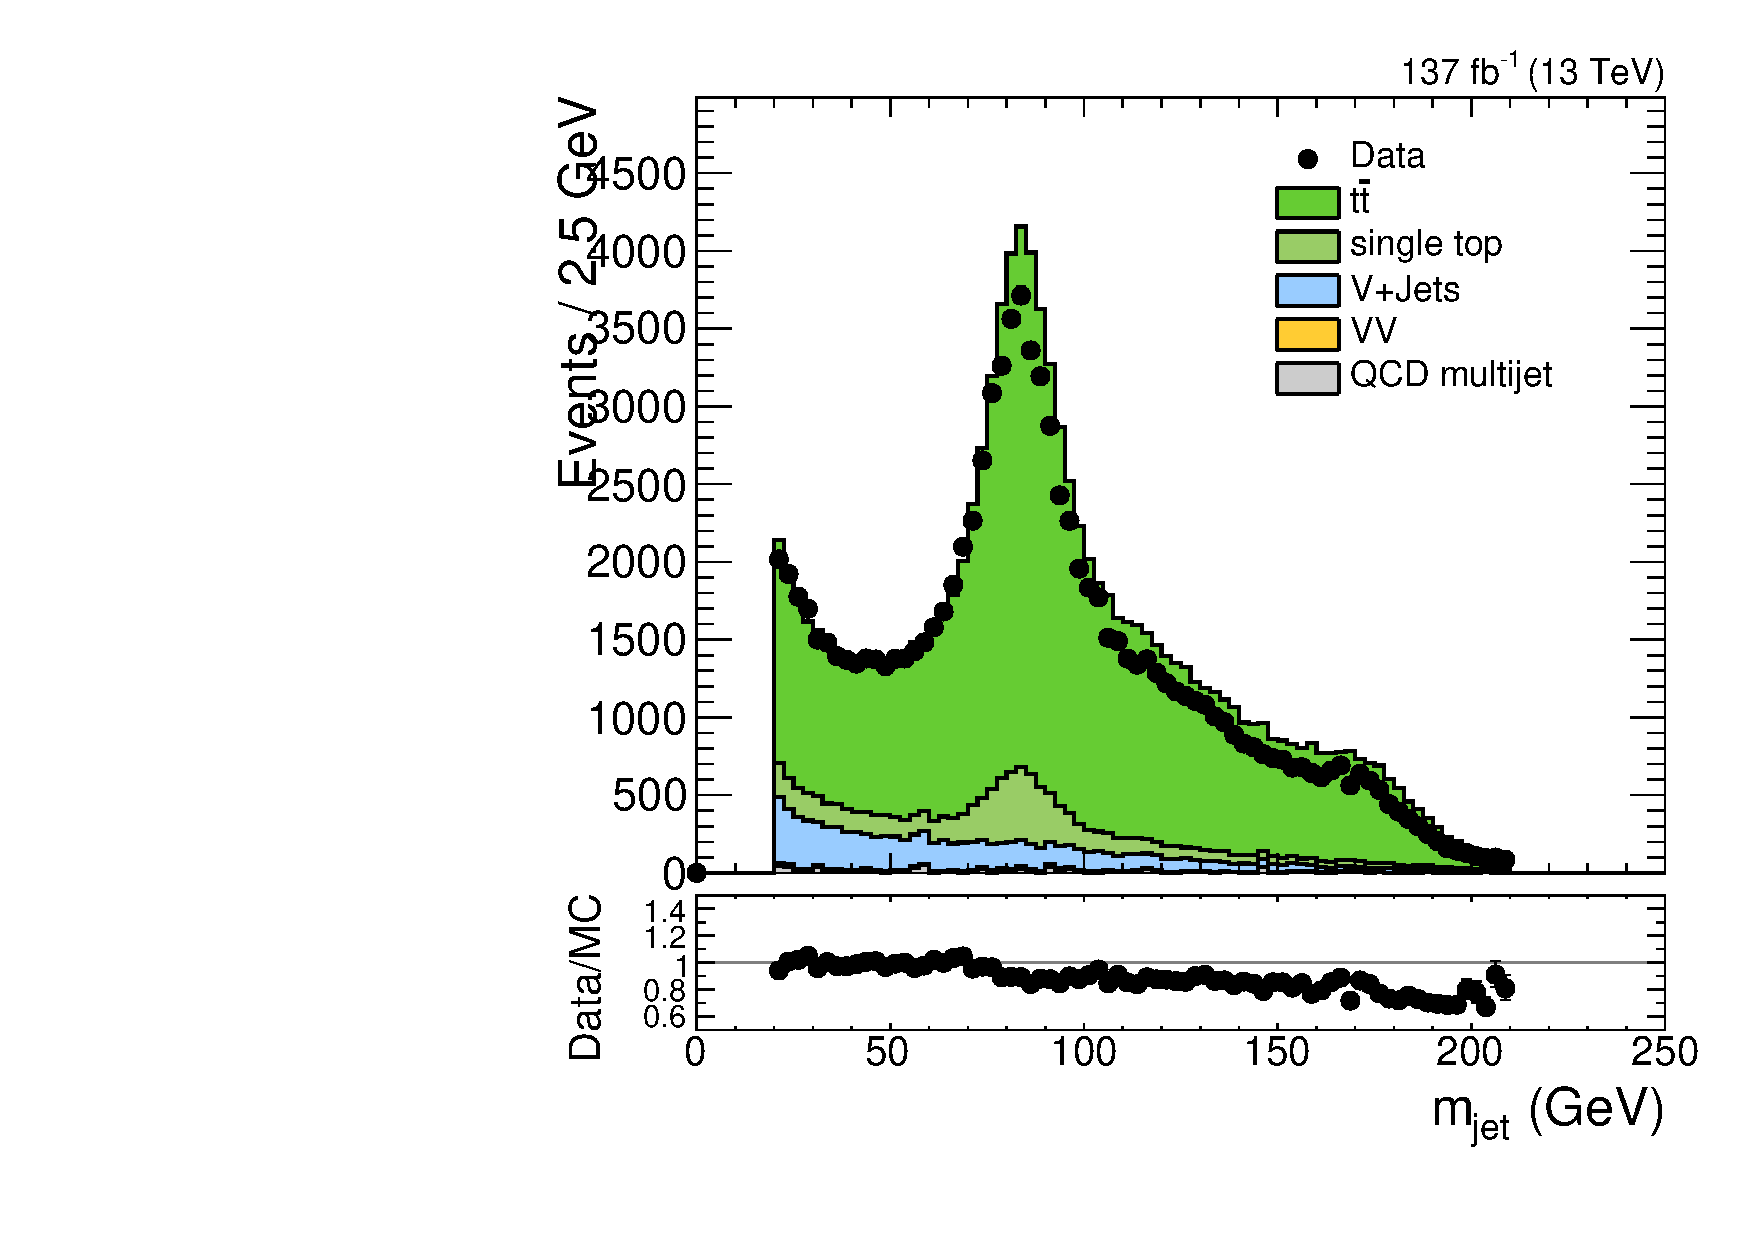
\includegraphics[width=0.3825\textwidth]{fig/controlPlots/CR_b1_allL_allP_allC_allD_Run2_mjet.pdf}\\
  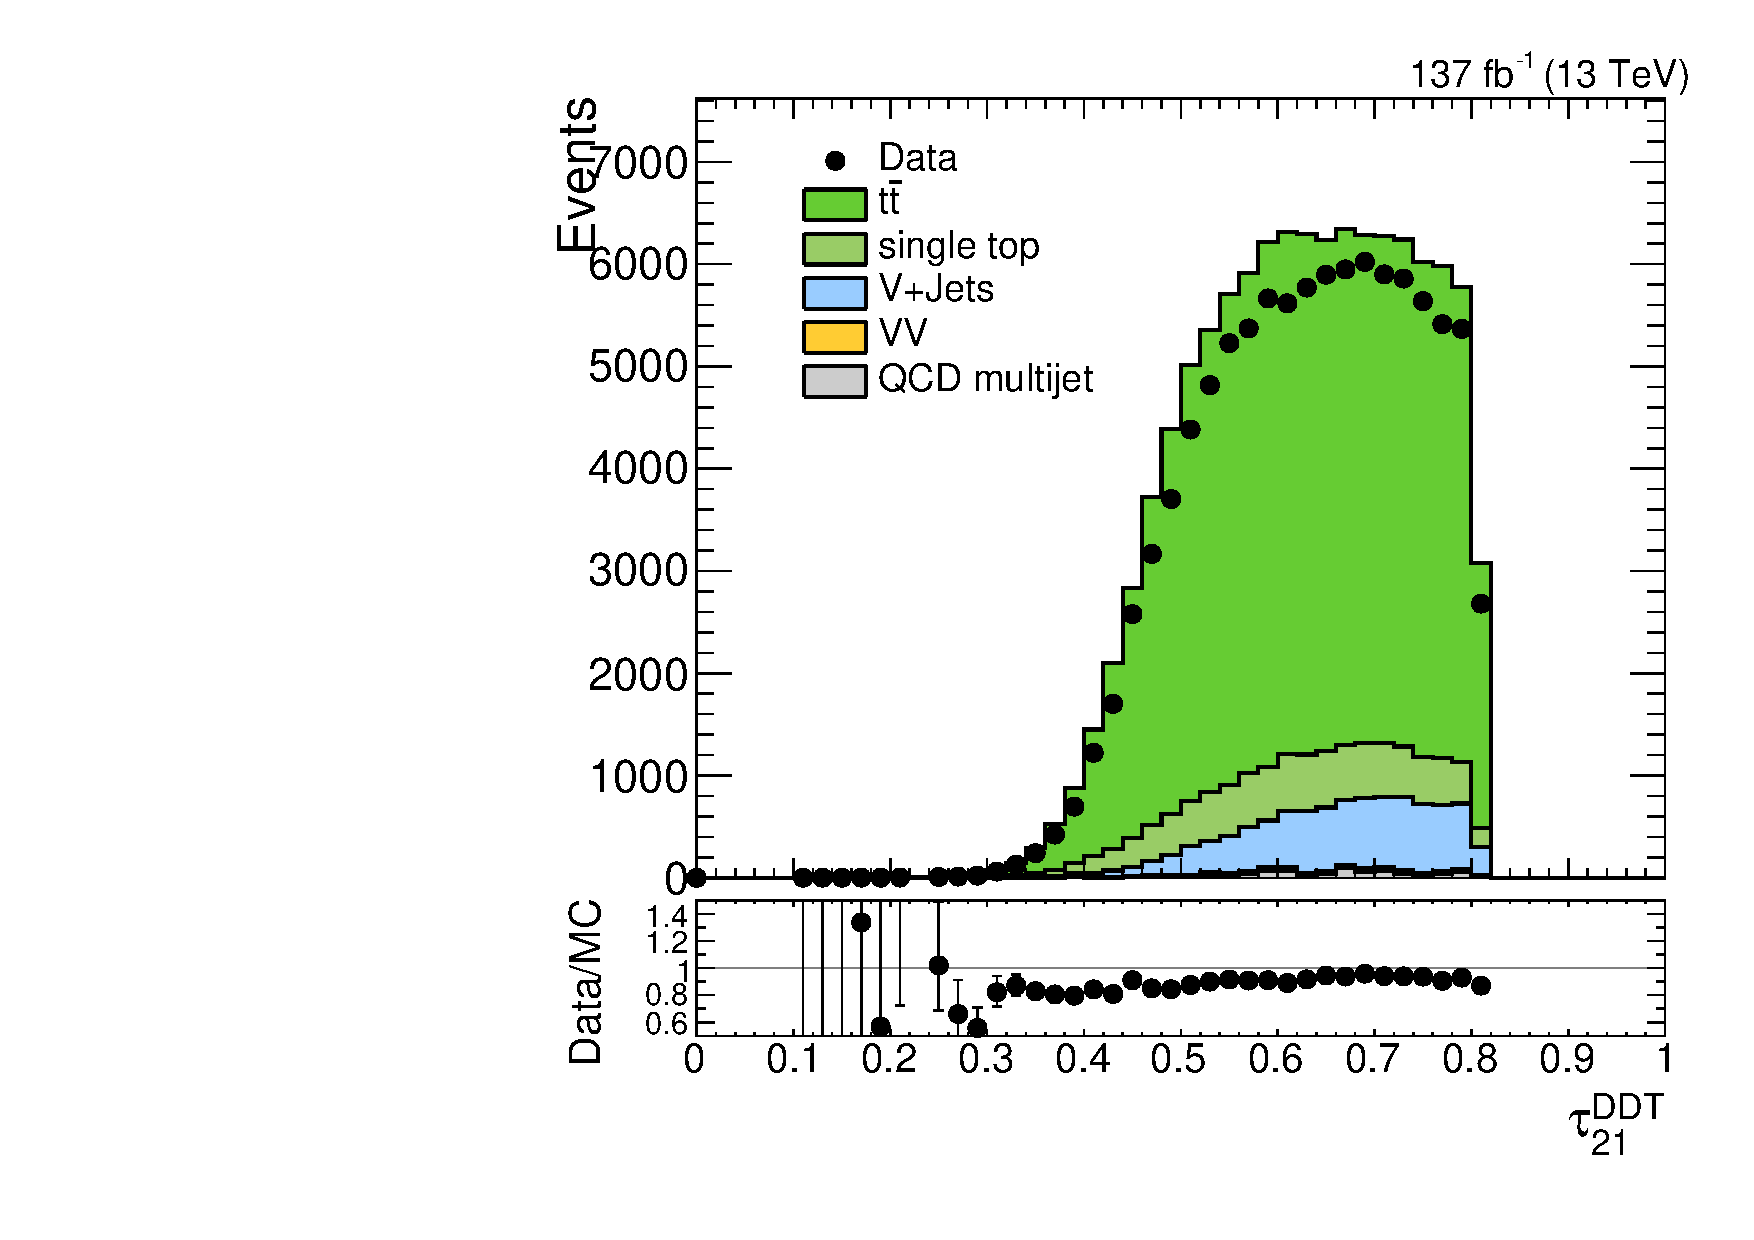
\includegraphics[width=0.3825\textwidth]{fig/controlPlots/CR_b1_allL_allP_allC_allD_Run2_tau21DDT.pdf}
  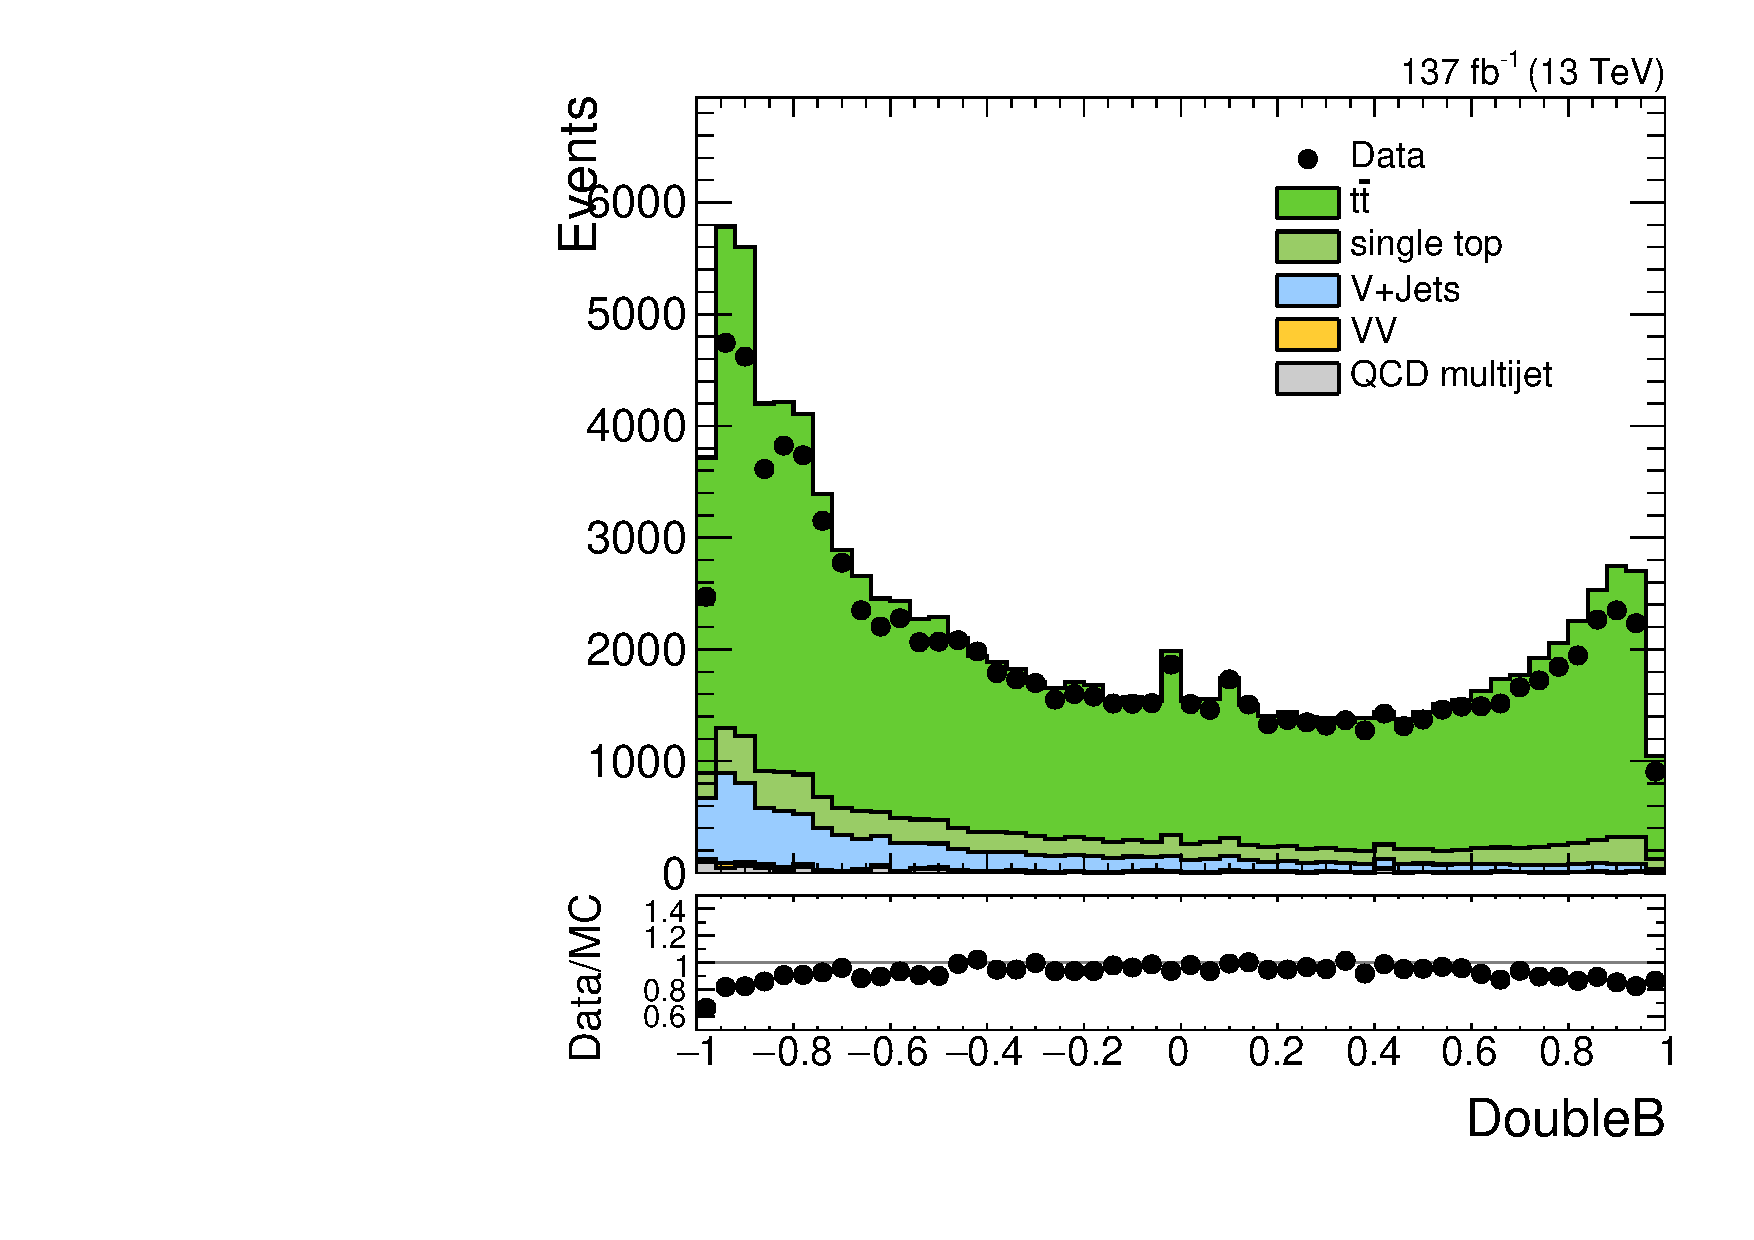
\includegraphics[width=0.3825\textwidth]{fig/controlPlots/CR_b1_allL_allP_allC_allD_Run2_DoubleB.pdf}\\
  \caption{
    Comparison plots between data and MC from Run 2 for the \pt, $\eta$, \MJ (soft drop mass), \nsubjDDT, and \DoubleB tagger of the selected \Vhad candidate (leading AK8 jet), in the top-enriched control region.
  }
  \label{fig:CR_controlPlotsRun2_3}
\end{figure}

\begin{figure}[htbp]
  \centering
  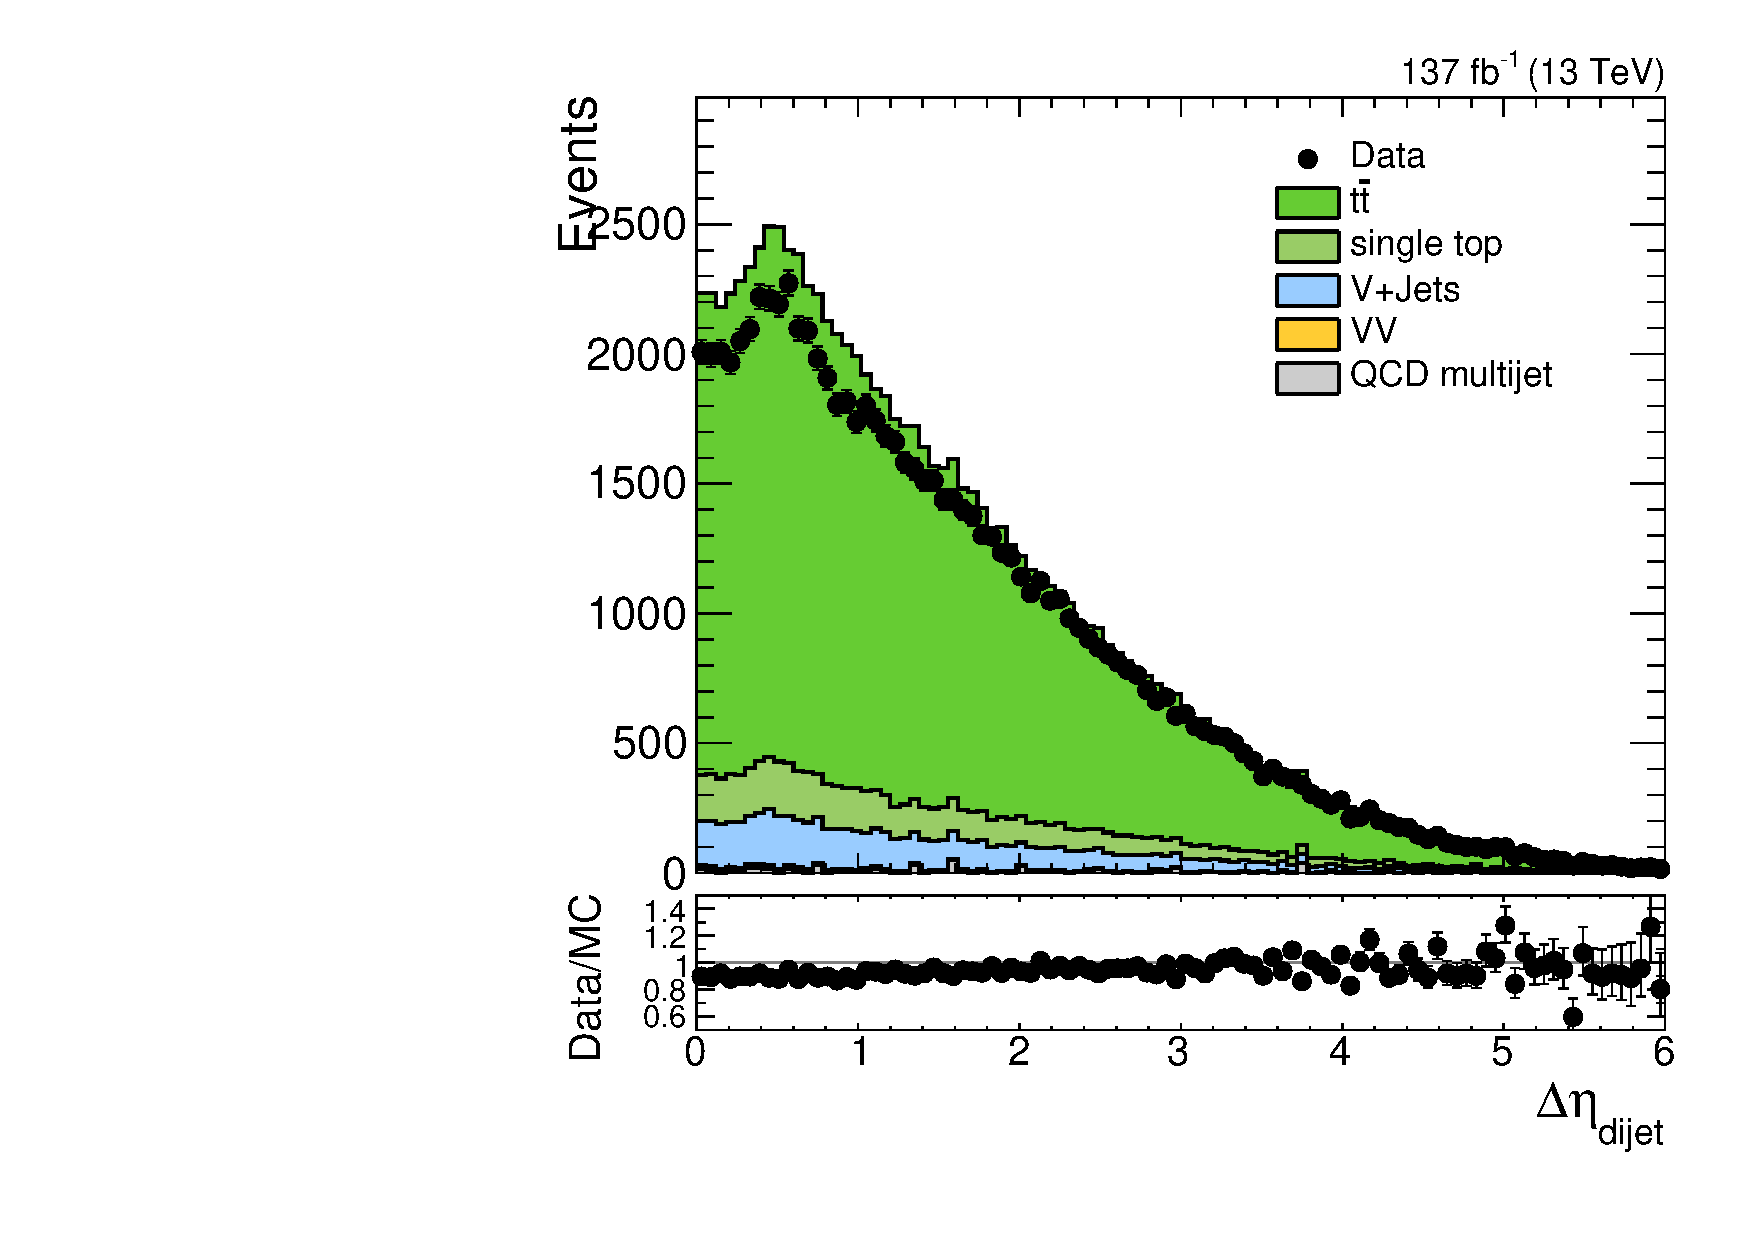
\includegraphics[width=0.3825\textwidth]{fig/controlPlots/CR_b1_allL_allP_allC_allD_Run2_lnujj_vbfDEta.pdf}
  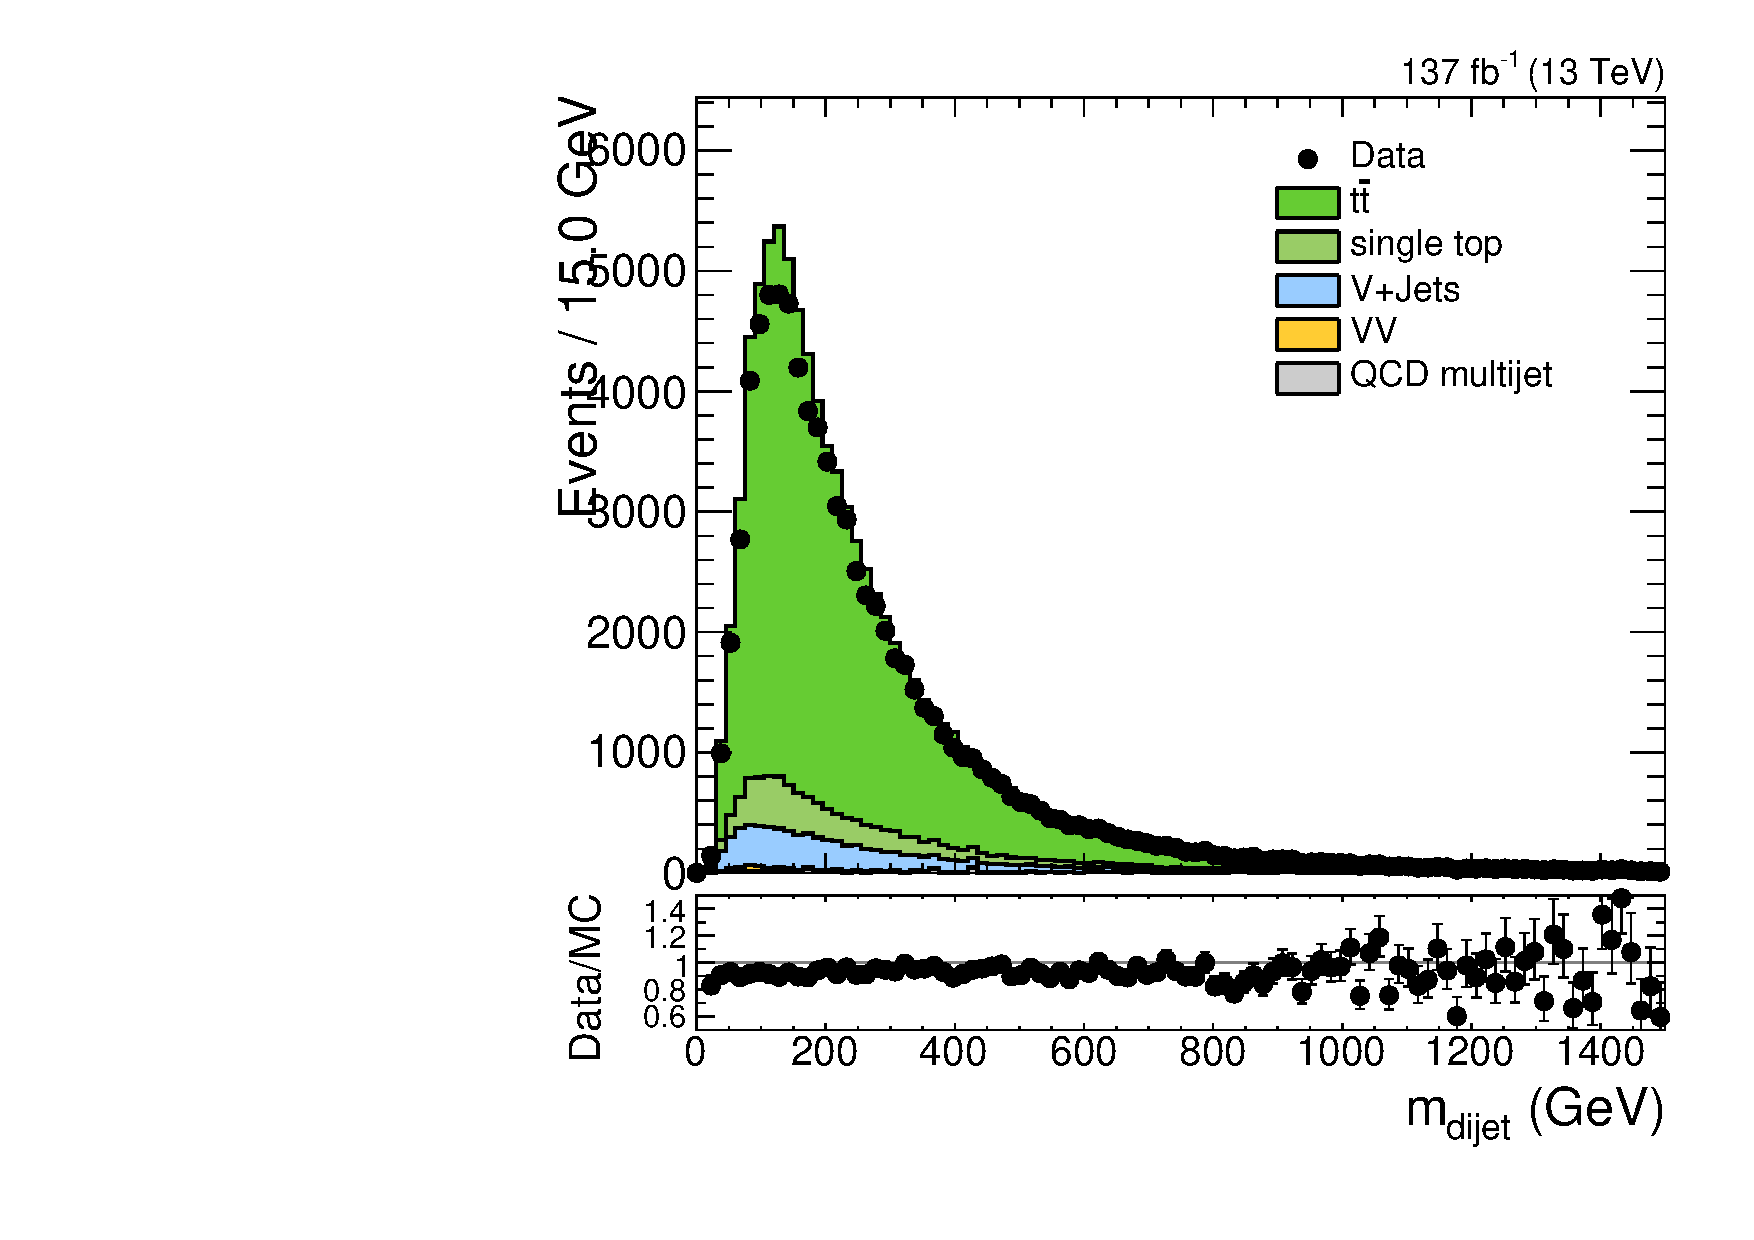
\includegraphics[width=0.3825\textwidth]{fig/controlPlots/CR_b1_allL_allP_allC_allD_Run2_lnujj_vbfMass.pdf}\\
  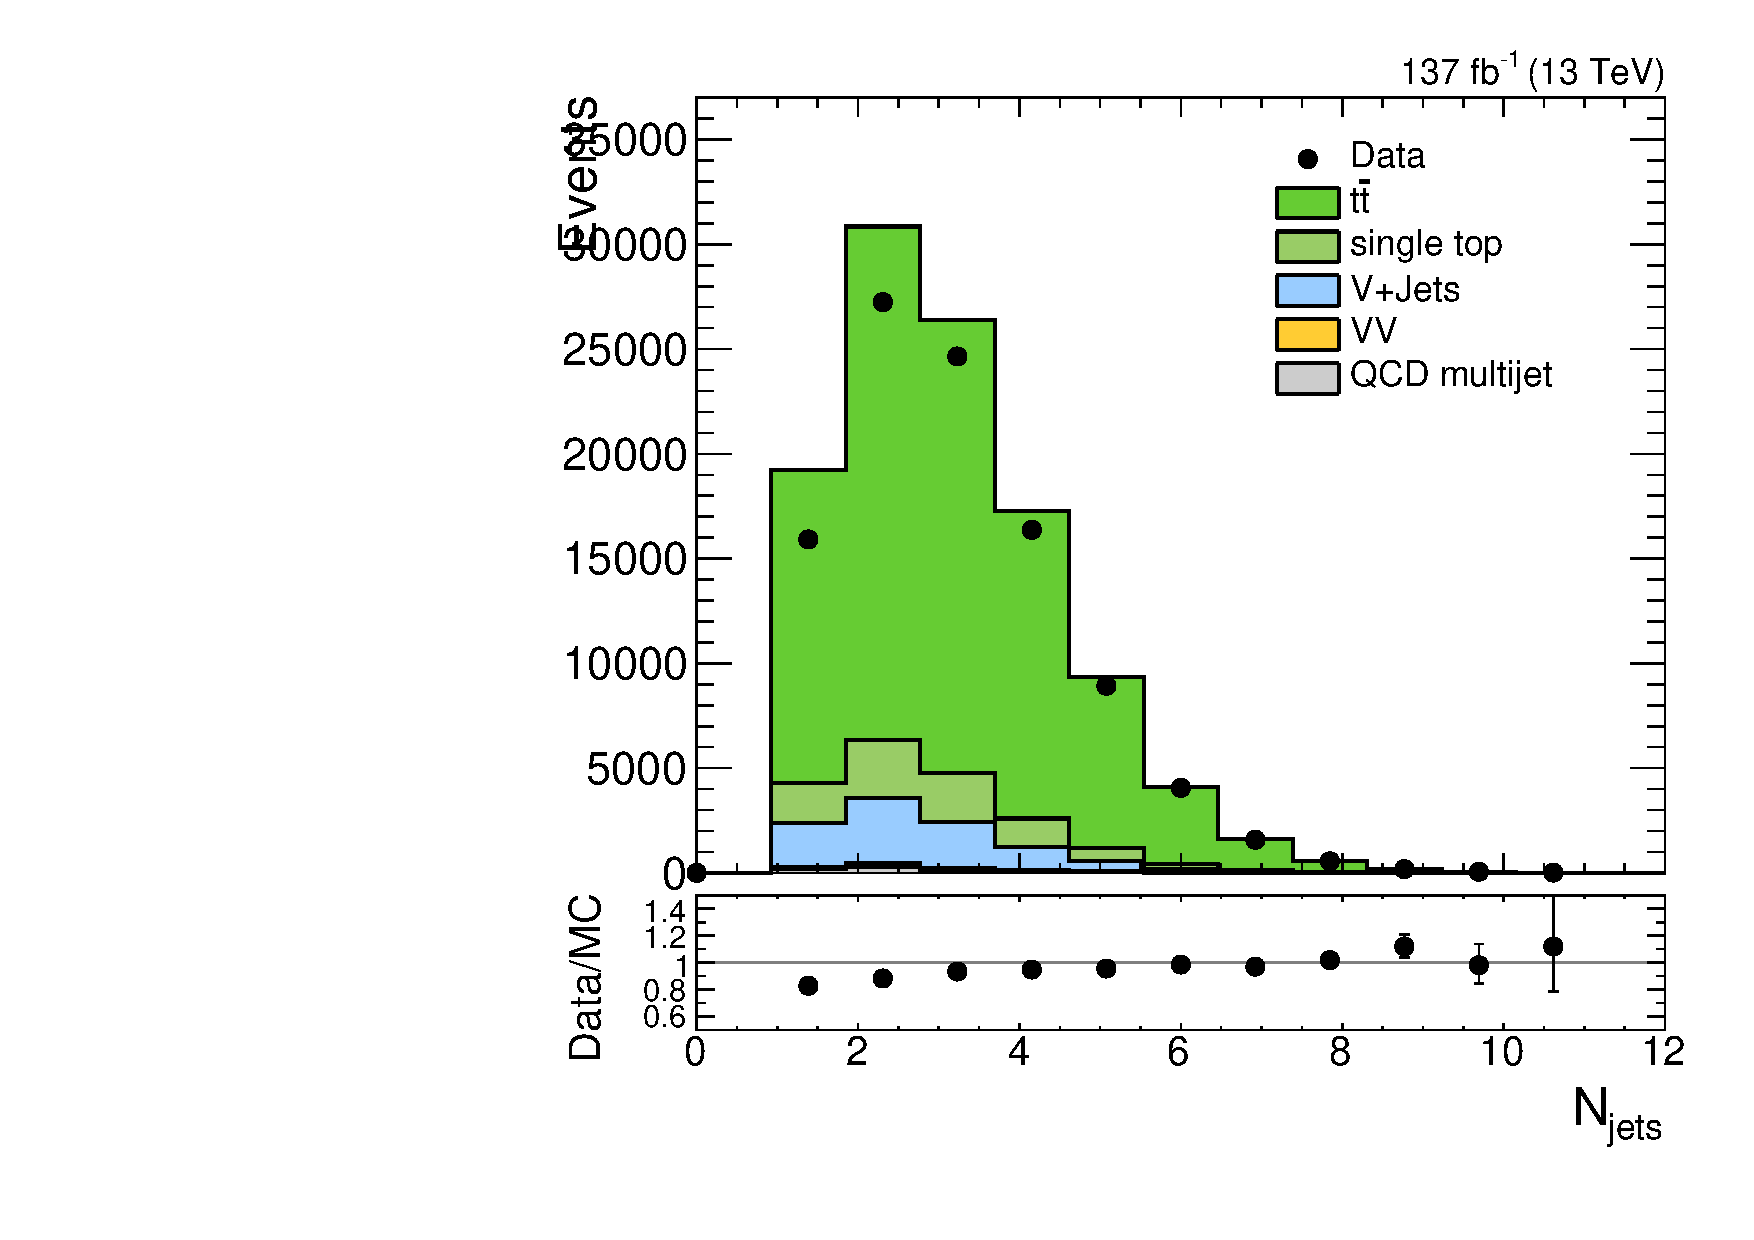
\includegraphics[width=0.3825\textwidth]{fig/controlPlots/CR_b1_allL_allP_allC_allD_Run2_lnujj_nJets.pdf}
  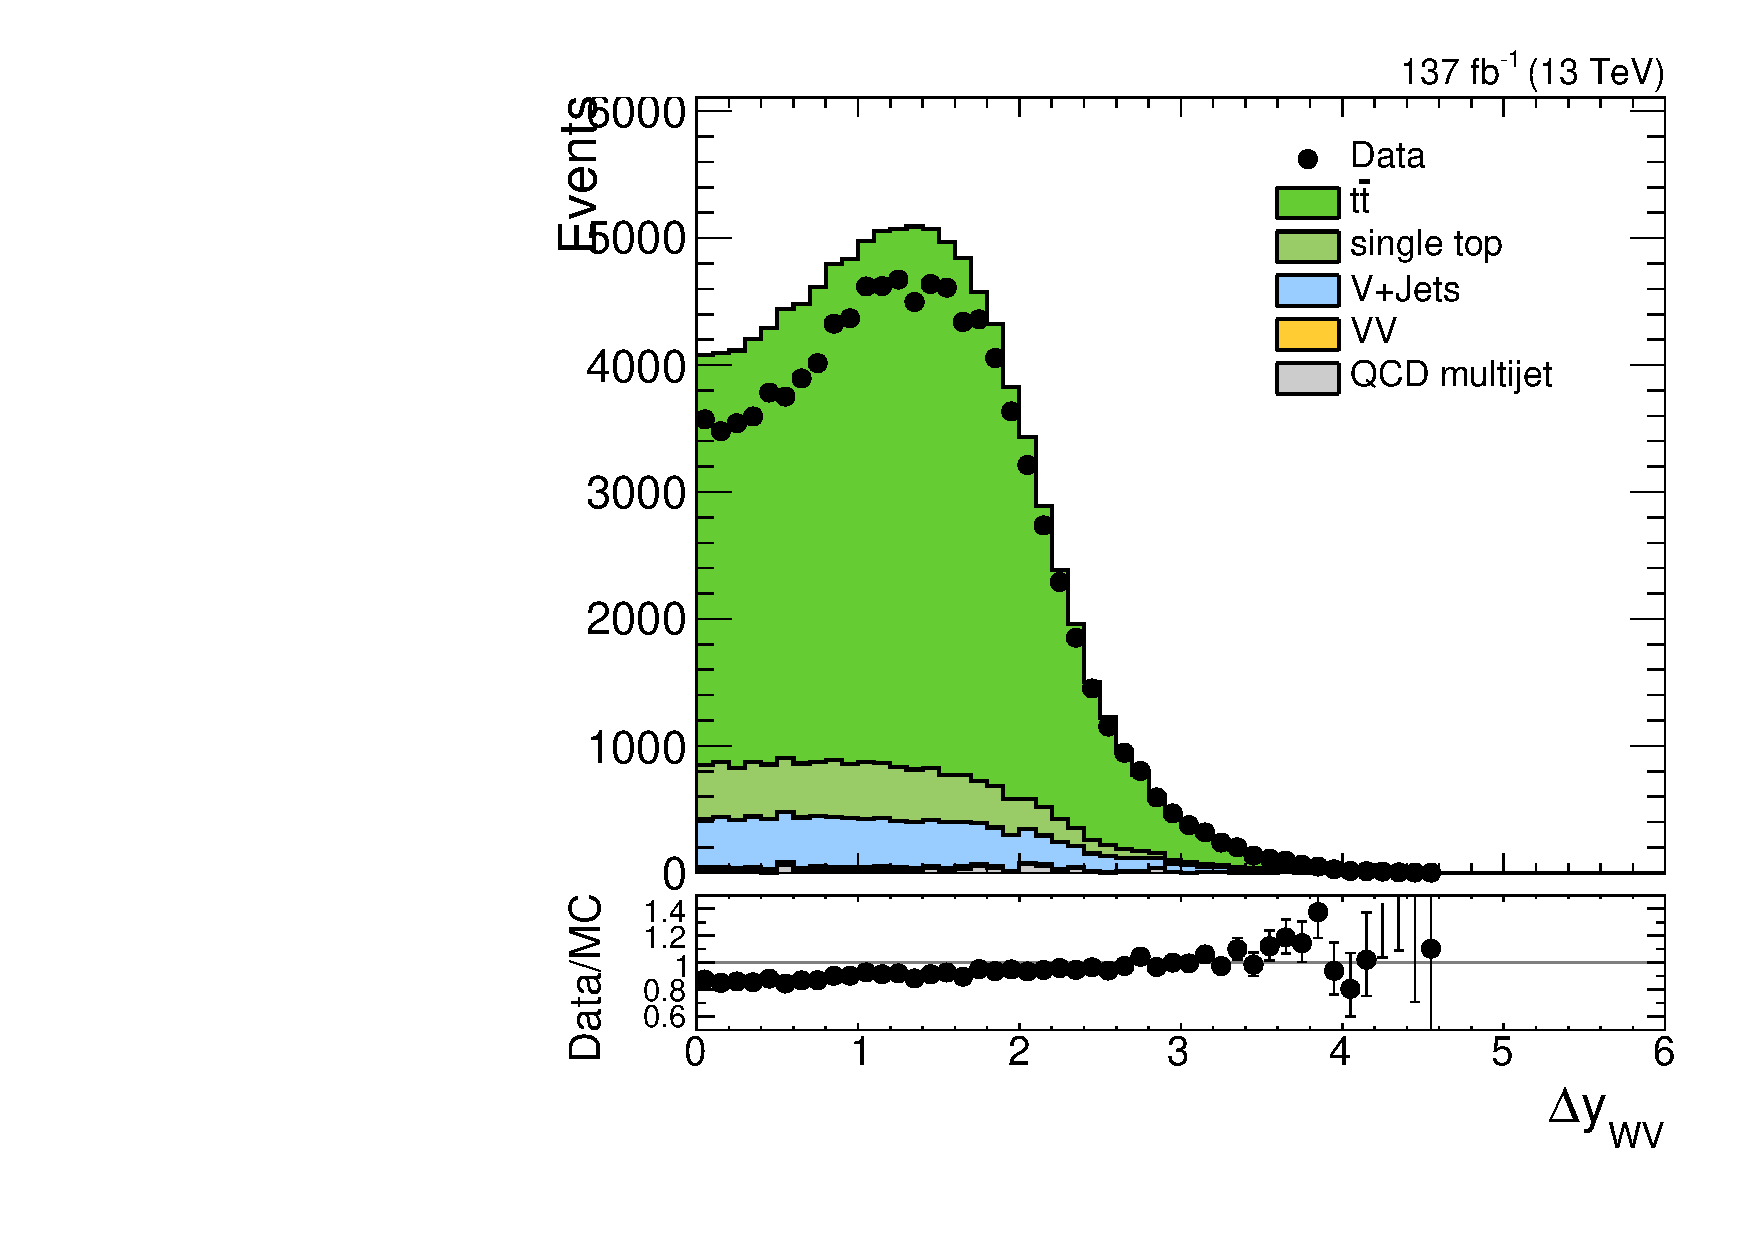
\includegraphics[width=0.3825\textwidth]{fig/controlPlots/CR_b1_allL_allP_allC_allD_Run2_dy.pdf}\\
  \caption{
    Comparison plots between data and MC from Run 2 for the separation in $\eta$ of the \VBF forward jets, invariant mass of the \VBF jets, number of selected standard jets, and rapidity separation between the reconstructed bosons, in the top-enriched control region.
  }
  \label{fig:CR_controlPlotsRun2_4}
\end{figure}

\subsection{Electron Negative Endcap Issue}

% Endcap issue
During Run 319077, the two HCAL towers HEM15 and HEM16 were non-operational, and the data obtained from the electron channel for the \Wtolnu candidate in those regions results in an excess of events that can be seen in figure~\ref{fig:SB_controlPlots2018_electronexcess}. % Citation
To remedy this, we exclude events recorded after Run 319077 if the lepton candidate is an electron and falls within the region $-1.55<\phi<-0.9$ and $-2.5<\eta<-1.479$.
Removing these events results in the correct behavior of the relevant kinematic variables for the electron candidate, and only discards 0.8\% of events in the signal region.

\begin{figure}[htbp]
  \centering
  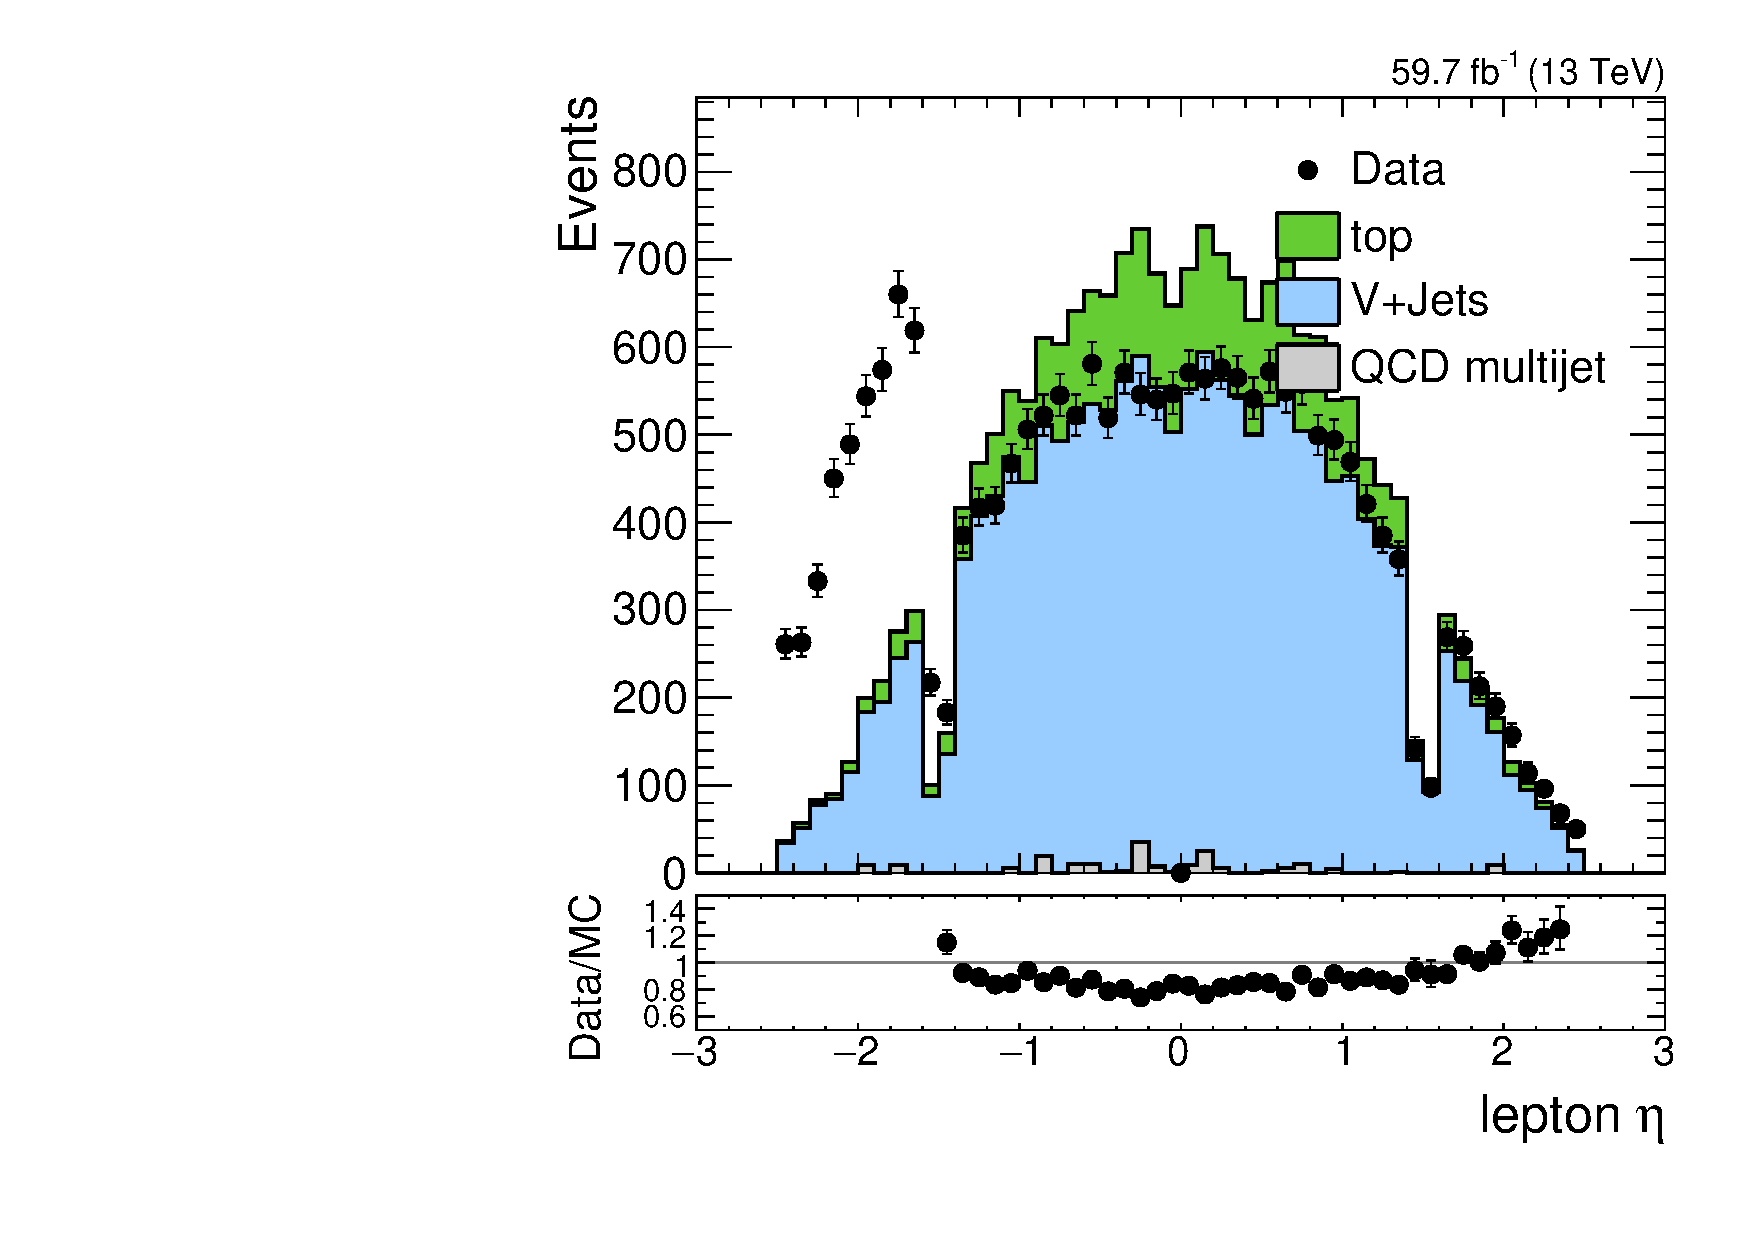
\includegraphics[width=0.30\textwidth]{fig/controlPlots/SB_e_2018_lnujj_l1_l_eta.pdf}
  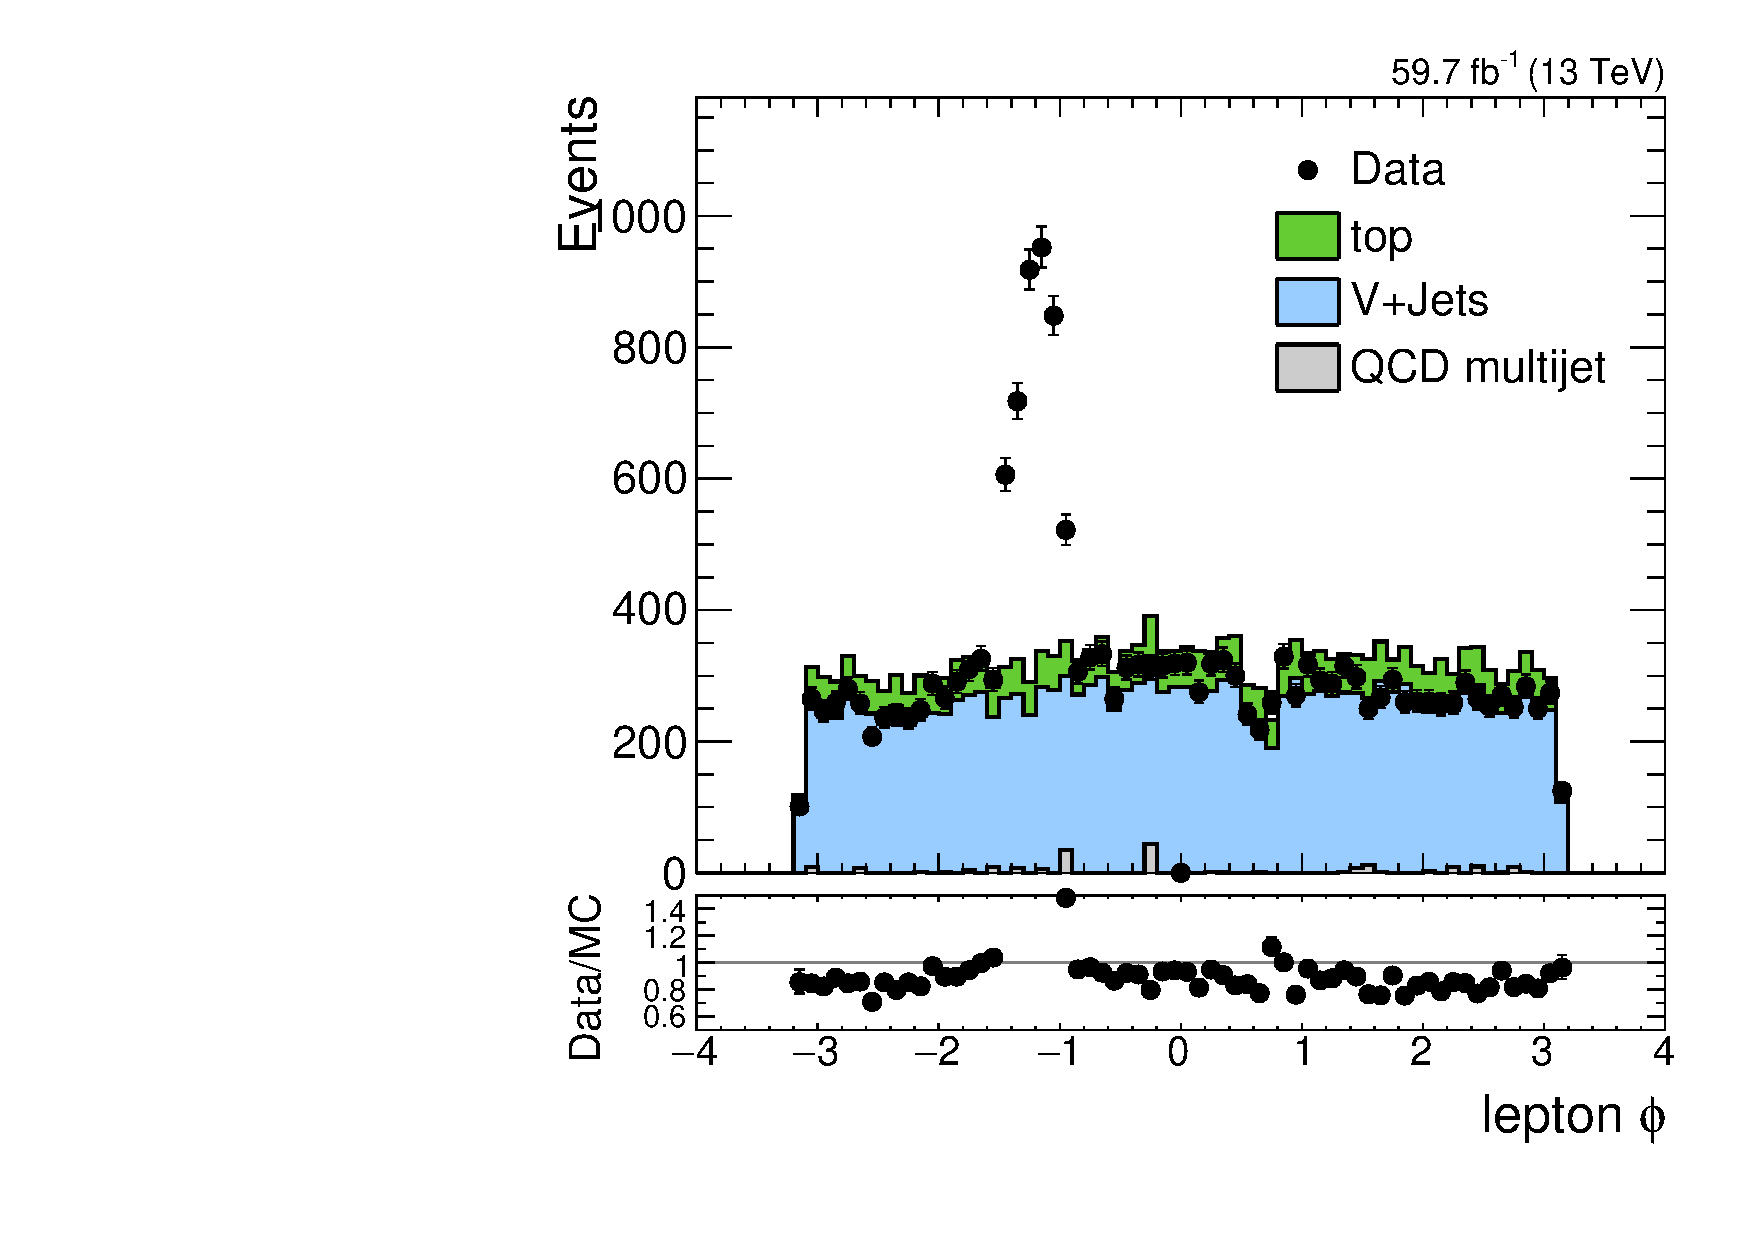
\includegraphics[width=0.30\textwidth]{fig/controlPlots/SB_e_2018_lnujj_l1_l_phi.pdf}
  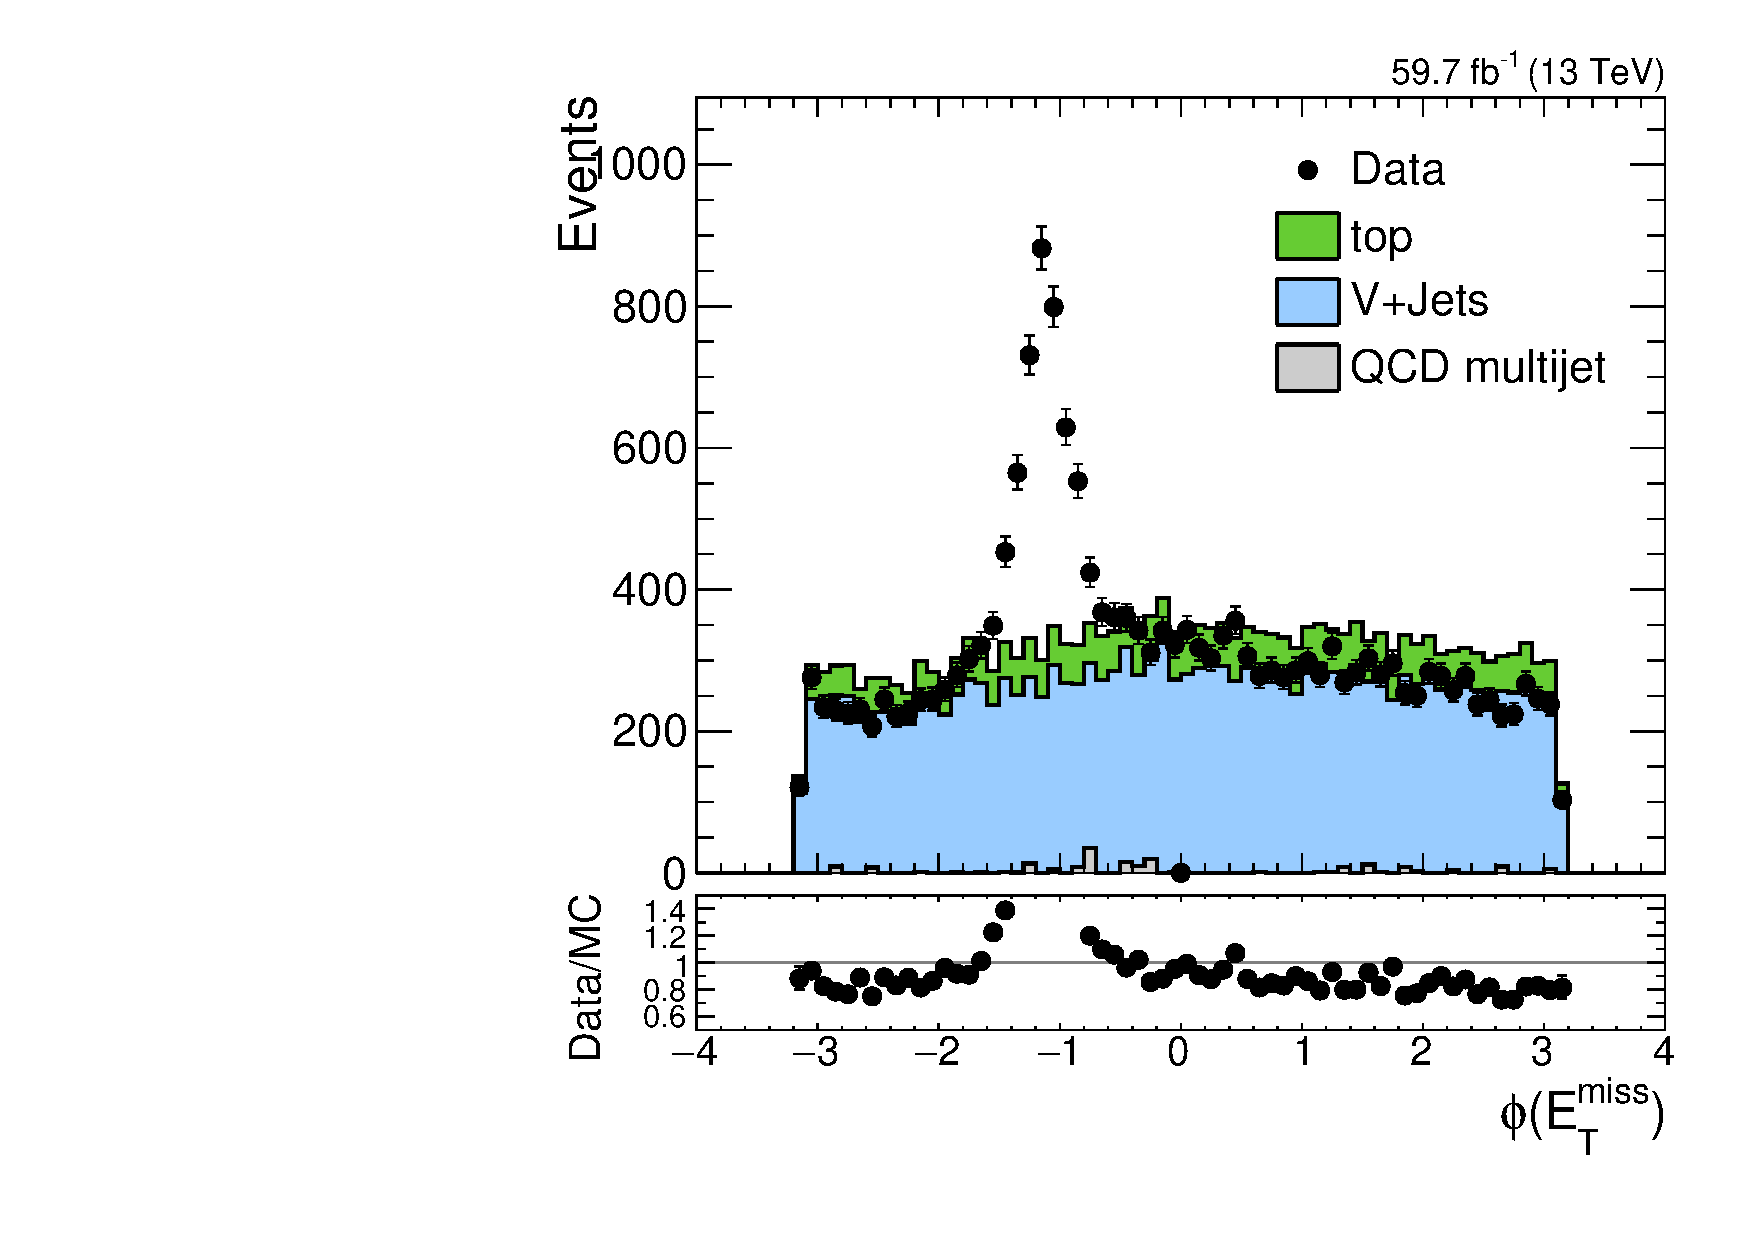
\includegraphics[width=0.30\textwidth]{fig/controlPlots/SB_e_2018_met_phi.pdf}
  \caption{
    Comparison plots between 2018 data (including the HEM15 and HEM16 after Run 319077) and 2017 MC for the electron $\eta$, electron $\phi$, and $\phi$ of the missing transverse energy, in the jet mass sideband.
  }
  \label{fig:SB_controlPlots2018_electronexcess}
\end{figure}

% Consider adding subsection for control plots in event categories
